\documentclass{book}
\usepackage[utf8]{inputenc}
\usepackage[T1]{fontenc}
\usepackage[T1]{fontenc}
\usepackage{graphicx}
\usepackage{apacite}
\usepackage{natbib}
\usepackage{float}
\usepackage{tikz}
\usepackage{array}
\usepackage{booktabs}
\usepackage{xcolor}
\usepackage{amsmath}
\usepackage{caption}
\usepackage{etoolbox}
\usepackage{pgfplots}
\usepackage{longtable}
\usepackage{lipsum}
\usetikzlibrary{positioning, arrows.meta, shapes.multipart}

%\addbibresource{referencias.bib}
\usetikzlibrary{positioning, arrows.meta, shapes.multipart}
\tolerance=1
\emergencystretch=\maxdimen
\hyphenpenalty=10000
\hbadness=10000
% Paquetes
%\usepackage[T1]{fontenc}
%\usepackage[spanish]{babel}
%\usepackage{hyperref}
%\usepackage{enumitem}
%\usepackage{geometry}
%\usepackage{fancyhdr}
%\usepackage{xcolor}
%\usepackage{url}
%\usepackage{listings}
%\lstset{breaklines=true}
\title{Trabajo de Grado}
\author{jjpaezr}
\date{April 2021}
%--------Configuración del tamaño de la hoja y sus margenes------
%\geometry{letterpaper,left=2.54cm,right=2.54cm,top=2.54cm,bottom=2.54cm}
%------------------Interlineado del documento--------------------
%\renewcommand{\baselinestretch}{1.6}
%--------------------------Sangria-------------------------------
%\setlength{\parindent}{0.5cm}
%---------------------Creación del documento----------------------

\usepackage{url}
\begin{document}
\begin{figure}[htb]
\centering

\includegraphics[width=55mm,scale=1]{escudo.png}
\end{figure}

\begin{center}\textbf{Uso de EEG para explorar la influencia de herramientas con agentividad en el control inhibitorio durante la resolución del juego La Escalera en niños con Trastorno del espectro Autista - TEA nivel 1}\end{center}
\vspace{45mm} %5mm vertical space
\begin{center}Nestor Andrés Paipa Castro \end{center}
\vspace{25mm} %5mm vertical space
\begin{center}Universidad Distrital Francisco José de Caldas\\
Facultad de Ciencias y Educación\\
Maestría en Educación en Tecnología\\
Bogotá\\
2026\end{center}
\newpage
%----------------------------------------------------------------
\begin{center}\textbf{Uso de EEG para explorar la influencia de herramientas con agentividad en el control inhibitorio durante la resolución del juego La Escalera en niños con Trastorno del espectro Autista - TEA nivel 1}\end{center}
\vspace{15mm} %5mm vertical space
\begin{center}Nestor Andrés Paipa Castro \end{center}
\vspace{20mm} %5mm vertical space
\begin{center}Herramientas con agentividad y su influencia en el control inhibitorio durante la resolución del juego La Escalera en niños con Trastorno del espectro Autista - TEA nivel 1\end{center}
\vspace{1mm} %5mm vertical space
\begin{center}Modalidad: Profundización\end{center}
\vspace{15mm} %5mm vertical space
\begin{center}Director\\
PhD Jhon Jairo Páez Rodríguez\end{center}
\vspace{45mm} %5mm vertical space
\begin{center}Universidad Distrital Francisco José de Caldas\\
Facultad de Ciencias y Educación\\
Maestría en Educación en Tecnología\\
Bogotá\\
2026\end{center}
\newpage
%----------------------------------------------------------------

ARTÍCULO 23, RESOLUCIÓN \#13 DE 1946 “La Universidad no se hace responsable por los conceptos emitidos por sus alumnos en sus trabajos de tesis. Sólo velará porque no se publique nada contrario al dogma y a la moral católica y porque las tesis no contengan ataques personales contra persona alguna, antes bien se vean en ellas el anhelo de buscar la verdad y la justicia” 
\newpage

%----------------------------------------------------------------
\begin{center}\textbf{Dedicatoria}\end{center}
\vspace{1mm} %5mm vertical space
\begin{center}Dedico este trabajo de grado a XXXX.\end{center} 
\newpage
%----------------------------------------------------------------
\begin{center}\textbf{Agradecimientos}\end{center}
\vspace{1mm} %5mm vertical space
\begin{center}Agradecido con XXXXX.  \end{center}
\begin{center}A todos los profesores de la Maestría en Educación XXXXXX.\end{center}
\newpage
%----------------------------------------------------------------
\tableofcontents
\listoffigures
\listoftables
%\maketitle
\chapter{Introducción}

\section{Contexto del problema}

El Trastorno del Espectro Autista es una condición del 
neurodesarrollo que afecta aproximadamente al uno por ciento 
de la población mundial, con variaciones en la prevalencia 
según los criterios diagnósticos y los sistemas de registro 
utilizados en cada país \cite{Lord2018, APA2022}. En Colombia, 
el reconocimiento institucional del TEA como condición que 
requiere atención educativa diferenciada ha avanzado 
progresivamente en el marco de la política de educación 
inclusiva, aunque persisten brechas significativas entre 
el diagnóstico clínico y la disponibilidad de estrategias 
pedagógicas fundamentadas en evidencia para atender las 
necesidades específicas de esta población en el aula 
\cite{Hirota2023}. En particular, los estudiantes con TEA 
nivel 1, quienes presentan lenguaje funcional y pueden 
acceder a contenidos académicos con relativa autonomía, 
suelen pasar desapercibidos durante periodos prolongados 
precisamente porque su perfil cognitivo no genera 
dificultades evidentes en tareas estructuradas y 
repetitivas, pero sí produce problemas significativos 
en situaciones que exigen planificación, flexibilidad 
y control voluntario del comportamiento 
\cite{APA2022, Happe2020}.

Estas dificultades tienen una base neurobiológica 
identificada en la literatura. El TEA nivel 1 se asocia 
con diferencias en la organización y maduración de las 
redes prefrontales que sustentan las funciones ejecutivas, 
es decir, el conjunto de procesos cognitivos que permiten 
regular la conducta, mantener información activa en la 
memoria de trabajo, cambiar de estrategia y suprimir 
respuestas automáticas en favor de acciones deliberadas 
\cite{Diamond2013, Hill2004}. Entre estos procesos, 
el control inhibitorio ocupa una posición central: 
es el mecanismo que permite detener una respuesta 
impulsiva, ignorar estímulos irrelevantes y mantener 
la conducta orientada hacia una meta cuando el entorno 
ofrece alternativas más inmediatas pero menos eficientes 
\cite{Diamond2013, Miyake2000}. Las investigaciones han 
mostrado que las personas con TEA nivel 1 pueden mostrar 
rendimiento adecuado en tareas simples de inhibición, 
pero presentan mayor variabilidad y mayor tasa de errores 
cuando la tarea exige inhibición sostenida bajo alta 
carga cognitiva o en presencia de interferencia emocional 
\cite{Geurts2009, Hill2004}. En el contexto escolar, 
esta dificultad se manifiesta cuando el estudiante debe 
resolver problemas que requieren organizar varios pasos 
en secuencia, evaluar consecuencias futuras de una 
decisión presente, o corregir una estrategia que no 
está funcionando sin perder el control de la conducta.

La resolución de problemas matemáticos constituye 
precisamente uno de los escenarios donde estas 
dificultades se hacen más visibles. Resolver un 
problema matemático no es un acto de recuperación 
de información almacenada: es un proceso de 
coordinación simultánea entre la memoria de trabajo, 
la flexibilidad cognitiva y el control inhibitorio, 
que exige mantener activa la representación del 
objetivo, inhibir rutas de solución que resultan 
atractivas pero ineficientes, y ajustar la estrategia 
en función de los resultados parciales obtenidos 
\cite{Diamond2013, Baddeley2000}. En tareas de 
transformación como el juego La Escalera, donde 
el objetivo es intercambiar la posición de dos 
conjuntos de fichas mediante movimientos regulados 
por reglas precisas, cada decisión modifica el 
espacio de soluciones disponibles para las 
decisiones siguientes, de modo que un movimiento 
impulsivo puede cerrar caminos que son difíciles 
de recuperar sin retroceder \cite{PaezGonzalez2022}. 
Investigaciones previas realizadas en la Universidad 
Distrital Francisco José de Caldas han mostrado que 
la solución de este juego activa procesos de 
razonamiento secuencial y formulación de patrones 
aritméticos, y que el análisis de las trayectorias 
de solución permite identificar momentos de bloqueo 
cognitivo y reorganización estratégica que resultan 
relevantes para comprender el funcionamiento 
ejecutivo en contextos de aprendizaje 
\cite{Cardenas2017, RodriguezLopez2017, Natalia2017}.

Frente a estas características, la investigación 
en educación y en interacción humano-tecnología 
ha explorado el potencial de las herramientas 
con agentividad como mediadoras del proceso 
cognitivo. Páez y González demostraron que un 
sistema robótico con capacidad de andamiaje, 
fundamentado en el modelo BDI de agentes 
inteligentes y en la teoría del flujo, producía 
trayectorias de solución más eficientes en 
estudiantes de educación básica durante la 
resolución de un juego de tablero, y que la 
efectividad de la intervención era mayor cuando 
respondía a las necesidades del aprendiz que 
cuando era iniciada de manera autónoma por el 
sistema \cite{PaezGonzalez2022}. Este hallazgo 
sugiere que la agentividad más efectiva en 
contextos educativos es la que combina la 
capacidad de ejecución precisa de la herramienta 
con el juicio situacional del docente. Para 
una población con TEA nivel 1, donde las 
señales verbales e instruccionales pueden generar 
sobrecarga o malinterpretarse, una herramienta 
que traduce ese juicio pedagógico en estímulos 
multisensoriales calibrados, como luz, vibración 
y sonido, ofrece un canal de mediación que no 
depende de la interpretación de normas sociales 
implícitas y que puede actuar directamente 
sobre el estado de activación del aprendiz 
en el momento en que el control inhibitorio 
se ve comprometido \cite{APA2022, Wood1976, 
PaezGonzalez2022}.


\section{Planteamiento del problema}

A pesar de la evidencia disponible sobre las 
dificultades en el control inhibitorio en el TEA 
nivel 1 y sobre el potencial de las herramientas 
con agentividad como mediadoras del proceso 
cognitivo, existe un vacío en la investigación 
respecto a cómo la activación de este tipo de 
herramientas en tiempo real, guiada por el juicio 
del docente, influye en la actividad cerebral 
asociada al control inhibitorio durante la 
resolución de problemas matemáticos en estudiantes 
con esta condición. La mayoría de los estudios 
sobre funciones ejecutivas en el TEA utilizan 
paradigmas experimentales altamente controlados, 
como tareas Go/No-Go o Stroop, que permiten 
precisión en la medición pero no reflejan las 
condiciones de una situación de aprendizaje real 
\cite{Geurts2009, Hill2004}. A su vez, las 
investigaciones sobre mediación tecnológica en 
educación raramente incorporan medidas 
neurofisiológicas que permitan observar si la 
intervención de la herramienta produce cambios 
en la actividad cerebral del aprendiz más allá 
del desempeño conductual observable 
\cite{PaezGonzalez2022}.

Esta investigación se sitúa en ese cruce y 
formula la siguiente pregunta:

\vspace{3mm}
\begin{center}
\textit{¿De qué manera la activación de herramientas 
con agentividad por parte del docente influye en 
el control inhibitorio, evidenciado mediante el 
análisis de la actividad EEG, durante la resolución 
del juego La Escalera en estudiantes con Trastorno 
del Espectro Autista nivel 1?}
\end{center}
\vspace{3mm}

\section{Justificación}

Esta investigación se justifica desde tres 
perspectivas complementarias.

Desde el punto de vista científico, el estudio 
contribuye a la comprensión del control inhibitorio 
en el TEA nivel 1 en condiciones de aprendizaje 
semiestructurado, un contexto que la literatura 
ha explorado de manera limitada en comparación 
con los paradigmas experimentales clásicos. 
El uso del EEG como herramienta de registro 
durante la sesión completa de resolución del 
juego permite obtener información sobre la 
dinámica cortical en condiciones más cercanas 
a las que ocurren en un entorno educativo real, 
lo que complementa los datos conductuales con 
evidencia neurofisiológica sobre el estado 
funcional de las redes ejecutivas durante 
la tarea \cite{Luck2014, Klimesch1999}. 
Al ser un estudio exploratorio con dos 
participantes, su aporte no es la generalización 
estadística sino la identificación de patrones 
de activación diferencial que orienten el 
diseño de investigaciones posteriores con 
mayor control experimental.

Desde el punto de vista tecnológico, la 
propuesta de cubos inteligentes controlados 
por el docente representa una evolución 
fundamentada del modelo de andamiaje 
robótico desarrollado por Páez y González, 
adaptada a las características de una 
población con TEA nivel 1 y a las limitaciones 
prácticas de los sistemas autónomos de 
reconocimiento del estado del aprendiz 
\cite{PaezGonzalez2022}. La distribución 
de la agentividad entre el cubo como 
ejecutor sensorial y el docente como agente 
interpretativo permite una mediación más 
ajustada al ritmo real del aprendiz, sin 
los problemas de artificialización del 
entorno ni de generación de ansiedad 
que los sistemas autónomos han reportado 
en investigaciones previas.

Desde el punto de vista pedagógico, el 
estudio aporta evidencia preliminar sobre 
el uso de herramientas multisensoriales 
como mediadoras del control inhibitorio 
en estudiantes con TEA nivel 1 en 
contextos de resolución de problemas 
matemáticos, un área en la que la 
investigación nacional y latinoamericana 
es aún escasa. La sistematización del 
guión experimental y del protocolo de 
activación de los cubos constituye 
además un insumo práctico para docentes 
que trabajan con esta población y que 
buscan estrategias de intervención 
con fundamento teórico y metodológico 
\cite{Diamond2013, APA2022}.

\section{Objetivos}

\subsection*{Objetivo general}

Explorar la influencia de herramientas con 
agentividad en el control inhibitorio, 
evidenciado mediante el análisis de la 
actividad EEG, durante la resolución del 
juego La Escalera en estudiantes con 
Trastorno del Espectro Autista nivel 1.

\subsection*{Objetivos específicos}

\begin{itemize}

    \item Revisar metodologías que utilizan 
    señales EEG para el estudio del control 
    inhibitorio en la resolución de problemas 
    matemáticos, con el fin de fundamentar 
    el enfoque de análisis espectral utilizado 
    en esta investigación.

    \item Implementar computacionalmente una 
    metodología de análisis de señales EEG 
    basada en potencia relativa alfa por canal 
    (Alpha TRP), que permita comparar la 
    actividad cortical entre sesiones con y 
    sin mediación de herramientas con 
    agentividad.

    \item Diseñar un ambiente de aprendizaje 
    con herramientas con agentividad que 
    favorezca el desarrollo del control 
    inhibitorio en estudiantes con Trastorno 
    del Espectro Autista nivel 1 durante la 
    resolución del juego La Escalera, 
    articulando el ciclo regulador 
    Pausar-Pensar-Actuar con los principios
    del andamiaje pedagógico.

    \item Analizar la actividad cortical y el 
    desempeño en el control inhibitorio durante 
    la resolución del juego La Escalera en 
    dos estudiantes con Trastorno del Espectro 
    Autista nivel 1, bajo condiciones de 
    mediación con herramientas con agentividad 
    activadas por el docente.

\end{itemize}






\chapter{Estado del Arte y Marco Teórico} %
\section{Herramientas con agentividad en educación}


En el contexto de los ambientes de aprendizaje, las herramientas  no son objetos neutros: su diseño, su comportamiento y su capacidad de respuesta ante las acciones del aprendiz determinan el tipo de mediación que ejercen sobre el proceso cognitivo. Pea señala que las herramientas tecnológicas pueden actuar como extensiones de la mente humana cuando están diseñadas para distribuir la carga cognitiva y reorganizar la estructura de la tarea, de manera que el aprendiz pueda operar en niveles de complejidad que no alcanzaría de forma independiente \cite{Pea2004}. Desde esta 
perspectiva, una herramienta adquiere agentividad cuando no se 
limita a responder pasivamente a las acciones del usuario, sino 
que puede iniciar estímulos, modular el ritmo de la actividad e 
influir en el estado cognitivo y emocional del aprendiz durante 
la resolución de un problema.

El concepto de andamiaje, formulado originalmente por Wood, Bruner 
y Ross a partir de la teoría de la zona de desarrollo próximo de 
Vygotsky, describe el proceso mediante el cual un agente más 
competente ofrece soporte ajustado a las necesidades del aprendiz, 
reduciendo progresivamente esa ayuda a medida que el aprendiz 
desarrolla sus propias capacidades \cite{Wood1976}. En los entornos 
de aprendizaje mediados por tecnología, este principio ha dado 
lugar a sistemas en los que herramientas físicas o digitales 
asumen funciones de andamiaje, regulando la intervención según 
el estado de la tarea y las características del aprendiz 
\cite{Pea2004}. La eficacia de este tipo de mediación depende, 
en gran medida, de la capacidad de la herramienta para actuar 
en el momento adecuado, con la intensidad apropiada y a través 
del canal sensorial más accesible para el aprendiz.

En el campo de la interacción humano-robot con propósitos 
educativos, Páez y González propusieron la arquitectura 
Human-Robot Scaffolding (HRS-EDU), un sistema multiagente 
fundamentado en el modelo BDI (creencias, deseos e intenciones) 
que regula el comportamiento de un robot según el estado 
cognitivo y emocional del aprendiz durante la resolución de un 
problema bien definido. La arquitectura organiza la intervención 
del robot en seis tipos de metas: desarrollo de habilidades, 
control cognitivo, control emocional, control del desafío, 
señales de vida y apoyo inmediato, y selecciona la meta de mayor 
prioridad según la situación del aprendiz en cada momento 
\cite{PaezGonzalez2022}. Los resultados de esa investigación, 
realizada con 53 estudiantes entre 10 y 13 años, mostraron que 
la mediación del robot produjo trayectorias de solución más 
cortas y eficientes, y que las intervenciones resultaron más 
efectivas cuando el aprendiz las solicitaba que cuando el sistema 
las iniciaba de forma autónoma \cite{PaezGonzalez2022}. Este 
hallazgo sugiere que la agentividad de la herramienta no opera 
de manera independiente del juicio pedagógico: su efectividad 
depende de la capacidad de quien media para interpretar la 
situación y decidir cuándo y cómo intervenir.

La presente investigación retoma este antecedente y lo adapta 
a una población con características cognitivas específicas y a 
un contexto en el que la mediación autónoma presenta limitaciones 
prácticas y éticas. En lugar de un robot antropomórfico con 
capacidad de reconocimiento autónomo del estado del aprendiz, 
se propone un sistema de cubos inteligentes controlados por el 
docente desde una interfaz remota. Estos cubos funcionan como 
actuadores físicos del juicio pedagógico: el docente observa 
la sesión, evalúa el estado cognitivo y emocional del estudiante, 
y activa la fase correspondiente del ciclo regulador 
(Pausar, Pensar, Actuar), que se materializa en el cubo mediante
tres canales de salida simultáneos: luz LED de color específico, 
vibración háptica de patrón regulado e indicación sonora de 
frecuencia predefinida.

Esta arquitectura distribuye la agentividad entre dos componentes: 
el docente, que aporta el juicio situacional y la decisión 
pedagógica, y el cubo, que aporta la ejecución multisensorial 
precisa y replicable. El cubo no es, en este sentido, un 
dispositivo pasivo que responde a la presión del aprendiz: 
es un agente físico que, activado por el docente, produce 
estímulos calibrados para influir en el estado de activación 
del estudiante, reducir la impulsividad, sostener la planificación 
o confirmar la toma de decisión. Desde el punto de vista del 
control inhibitorio, esta mediación multisensorial busca 
convertir el entorno inmediato en una señal externa de regulación 
ejecutiva, reduciendo la dependencia de la instrucción verbal 
y ofreciendo al estudiante con TEA nivel 1 un canal de 
comunicación que no depende exclusivamente de la interpretación 
de normas sociales implícitas \cite{Wood1976, PaezGonzalez2022}.

La decisión de situar la agentividad en el sistema cubo-docente, 
en lugar de en un robot autónomo, responde también a las 
limitaciones identificadas en investigaciones previas. Páez y 
González señalaron que el reconocimiento autónomo del estado 
emocional requería una proximidad física a las cámaras que 
artificializaba el entorno experimental, y que las intervenciones 
autónomas del robot podían generar ansiedad cuando el aprendiz 
ya había comprendido la solución pero debía esperar a que el 
robot terminara su movimiento \cite{PaezGonzalez2022}. El diseño 
propuesto en esta investigación supera esas limitaciones al 
mantener al docente como agente interpretativo y al cubo 
como ejecutor sensorial, lo que permite una respuesta más 
ajustada al ritmo real del aprendiz con TEA nivel 1.

\subsection{El juego La Escalera como problema matemático 
bien definido}

En el diseño de ambientes de aprendizaje para el estudio de 
procesos cognitivos, la selección de la tarea no es un detalle 
secundario: determina qué procesos pueden observarse, con qué 
precisión y en qué condiciones. Para que una tarea permita 
analizar el control inhibitorio de manera sistemática, debe 
cumplir condiciones específicas: tener un espacio de solución 
claramente delimitado, requerir decisiones sucesivas donde la 
respuesta impulsiva conduzca a errores recuperables, y no 
depender de conocimiento previo especializado que introduzca 
variabilidad irrelevante \cite{PaezGonzalez2022, Diamond2013}. 
El juego La Escalera satisface estas condiciones y ha sido 
utilizado en investigaciones previas como dispositivo para 
estudiar el pensamiento matemático, la formulación de patrones 
y la resolución de problemas en contextos educativos colombianos 
\cite{Cardenas2017, RodriguezLopez2017, Natalia2017}.

\begin{figure}[h]
    \centering
        \caption{Explicación Juego}
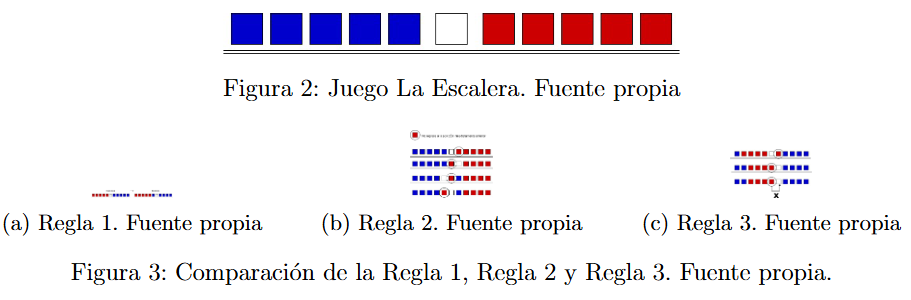
\includegraphics[width=0.50\textwidth]{juego.png}
\begin{flushleft}
\footnotesize
\textit{Nota.} Elaboración propia.
\end{flushleft}
\label{juegoreglas}
\end{figure}
La Escalera es un problema de transformación con espacio de 
estados bien definido. El tablero consiste en una fila lineal 
de once posiciones: cinco fichas de un color ocupan las 
posiciones del extremo izquierdo, cinco fichas de un segundo 
color ocupan las posiciones del extremo derecho, y una posición 
central permanece vacía al inicio. El objetivo del juego es 
intercambiar completamente la posición de ambos conjuntos de 
fichas, de manera que las fichas que comenzaron a la izquierda 
terminen a la derecha y viceversa. El juego se rige por dos 
operadores: una ficha puede avanzar una posición hacia el centro 
si la posición inmediata siguiente está vacía, o puede saltar 
sobre una ficha del color contrario si la posición después de 
esa ficha está vacía. En ambos casos el movimiento es 
unidireccional: las fichas del grupo izquierdo solo avanzan 
hacia la derecha, y las del grupo derecho solo avanzan hacia 
la izquierda. No se permiten retrocesos \cite{PaezGonzalez2022}.

Desde el punto de vista matemático, el espacio de estados del 
juego puede representarse como un grafo dirigido en el que cada 
nodo corresponde a una configuración posible del tablero y cada 
arco representa un movimiento válido según los operadores 
descritos. El camino óptimo de solución, calculado mediante 
el patrón alternado de movimientos individuales y saltos, 
requiere exactamente 35 movimientos para la versión de cinco 
fichas por lado, resultado que se obtiene de la expresión 
general $n^2 + 2n$, donde $n$ representa el número de fichas 
por conjunto \cite{PaezGonzalez2022}. Sin embargo, los 
aprendices que enfrentan el juego por primera vez, sin conocer 
la estrategia de análisis de medios y fines, suelen superar 
ampliamente ese número de movimientos, produciendo ciclos y 
retrocesos que reflejan decisiones impulsivas no planificadas. 
La diferencia entre el camino óptimo y el camino real del 
aprendiz constituye una medida observable de la planificación 
y del control inhibitorio: a mayor cantidad de ciclos y 
movimientos redundantes, mayor evidencia de dificultad para 
inhibir la respuesta impulsiva y sostener una estrategia 
deliberada \cite{Diamond2013, Hill2004}.

\begin{figure}[h]
    \centering
        \caption{Espacio del problema. xxxxxx}
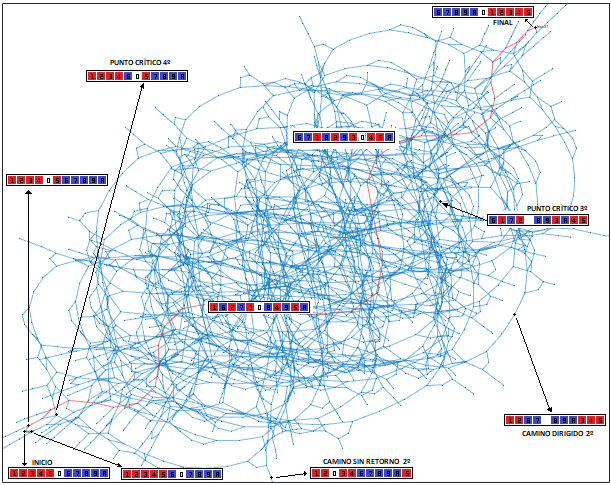
\includegraphics[width=0.50\textwidth]{Grafo.png}
\begin{flushleft}
\footnotesize
\textit{Nota.} Elaboración propia.
\end{flushleft}
\label{MWM1}
\end{figure}
Esta característica convierte a La Escalera en un escenario 
especialmente adecuado para el estudio del control inhibitorio 
en estudiantes con TEA nivel 1. Cada vez que el aprendiz 
enfrenta la decisión de mover una ficha, debe evaluar si ese 
movimiento contribuye al objetivo final o si, aunque sea 
permitido por las reglas, conduce a un estado desde el que 
la solución se vuelve más difícil o imposible. Inhibir el 
movimiento inmediato disponible en favor de una secuencia 
planificada más eficiente requiere exactamente los procesos 
que se encuentran alterados en el TEA nivel 1: supresión de 
la respuesta automática, mantenimiento de la meta en la 
memoria de trabajo y evaluación de consecuencias futuras 
\cite{Geurts2009, Diamond2013}. Investigaciones previas en 
el contexto de la Universidad Distrital han mostrado que la 
solución del juego activa procesos de formulación de patrones 
aritméticos y de razonamiento secuencial, y que el análisis 
de las trayectorias de solución permite identificar momentos 
críticos de bloqueo cognitivo y reorganización de la estrategia 
\cite{Cardenas2017, RodriguezLopez2017, Natalia2017}.

En el diseño experimental de la presente investigación, los 
cubos inteligentes se integran físicamente en el tablero de 
juego como elementos del entorno inmediato del aprendiz. Cada 
cubo es activado por el docente desde una interfaz remota en 
el momento en que, según su observación de la sesión, el 
estudiante muestra señales de impulsividad inminente, 
dificultad en la planificación o necesidad de confirmación 
de una decisión tomada. La activación del cubo no interrumpe 
el juego con instrucción verbal: introduce una señal 
multisensorial (luz LED, vibración háptica y sonido) que 
actúa directamente sobre el estado de activación del aprendiz 
sin requerir que este interprete lenguaje, intención social 
ni normas implícitas de interacción. Esta condición resulta 
especialmente relevante en el TEA nivel 1, donde las 
dificultades en la comprensión de señales sociales verbales 
pueden interferir con la regulación del comportamiento en 
contextos de demanda cognitiva \cite{APA2022, Happe2020}.

\begin{figure}[h]
    \centering
        \caption{Explicación del grafo en función de lo que paso con ese sujeto. Revisar la tesis de Rafael y Lina xxxxxx}
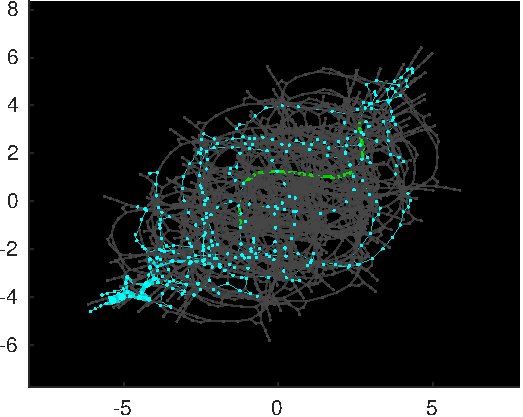
\includegraphics[width=0.80\textwidth]{GJRTI.pdf}
\begin{flushleft}
\footnotesize
\textit{Nota.} Elaboración propia.
\end{flushleft}
\label{MWM1}
\end{figure}

La combinación del juego La Escalera como tarea cognitiva 
estructurada, los cubos inteligentes como sistema de mediación 
multisensorial y el electroencefalograma como instrumento de 
registro de la actividad cerebral durante la sesión completa 
permite explorar, de manera integrada, la relación entre la 
actividad cortical, el control inhibitorio y la influencia 
de herramientas con agentividad en el desempeño de estudiantes 
con TEA nivel 1. La siguiente sección describe los fundamentos 
del análisis electroencefalográfico utilizado en esta 
investigación y su pertinencia para el estudio de procesos 
ejecutivos durante tareas de resolución de problemas.

\textcolor{red}{
\textbf{NOTA DE PENDIENTE — Referencias [11], [47] y [62] del artículo 
PaezGonzalez2022:} Verificar en el repositorio de la Universidad 
Distrital los datos completos de los tres trabajos de grado sobre 
La Escalera antes de la versión final. Confirmar: (1) nombre completo 
de los autores, (2) año exacto de publicación, (3) título exacto del 
documento. Las entradas actuales en bibliografia.bib 
(Cardenas2017, RodriguezLopez2017, Natalia2017) están basadas en 
las referencias del artículo y pueden contener datos incompletos. 
Corroborar y corregir en el arcvivo .bib
}


\subsection{Análisis espectral EEG y potencia alfa en tareas 
de control inhibitorio}

El electroencefalograma permite analizar la actividad cerebral 
desde dos perspectivas complementarias. La primera, basada en 
potenciales relacionados con eventos (ERP), examina cambios 
transitorios en la señal eléctrica que ocurren en respuesta a 
estímulos discretos y cuyo análisis requiere la repetición 
controlada de un mismo evento para extraer la señal del ruido 
de fondo mediante promediado. La segunda perspectiva, basada 
en el análisis espectral de la señal, examina la distribución 
de potencia eléctrica en diferentes bandas de frecuencia 
durante periodos sostenidos de actividad, lo que permite 
observar el estado funcional del cerebro a lo largo de una 
tarea completa sin requerir la segmentación en eventos 
discretos \cite{Luck2014, Uhlhaas2006}. Ambas aproximaciones 
son complementarias: mientras los ERP capturan la respuesta 
puntual del sistema nervioso ante un estímulo, el análisis 
espectral refleja la dinámica sostenida de las redes neuronales 
durante la ejecución de una tarea cognitiva.

Dentro del análisis espectral, la banda de frecuencia alfa 
(8--13 Hz) ha recibido especial atención en la investigación 
sobre funciones ejecutivas y control cognitivo. La potencia 
alfa cortical muestra una relación inversa con el nivel de 
activación y procesamiento de una región: cuando una zona del 
cortex está activamente implicada en una tarea, su potencia 
alfa disminuye, fenómeno denominado desincronización alfa o 
supresión alfa relacionada con eventos. Por el contrario, 
cuando una región no está siendo reclutada para la tarea en 
curso, su potencia alfa aumenta, lo que refleja un estado 
de inhibición activa o de procesamiento reducido 
\cite{Klimesch1999, Pfurtscheller1999}. Este mecanismo 
convierte a la potencia alfa en un índice sensible al estado 
de activación de las redes prefrontales y parietales que 
sostienen el control inhibitorio, la memoria de trabajo y 
la regulación del comportamiento.

Una métrica derivada del análisis espectral que ha ganado 
relevancia en investigaciones sobre cognición y aprendizaje 
es la potencia relativa alfa por canal, también referida 
como Alpha TRP (Task-Related Power). Esta métrica cuantifica 
la proporción de potencia espectral correspondiente a la 
banda alfa en cada electrodo durante la realización de una 
tarea, permitiendo comparar el nivel de activación cortical 
entre regiones cerebrales, entre condiciones experimentales 
y entre sesiones de un mismo participante \cite{Klimesch1999}. 
A diferencia de los componentes ERP, que requieren múltiples 
ensayos idénticos para su cálculo, el Alpha TRP puede 
estimarse a partir de segmentos continuos de señal, lo que 
lo hace especialmente adecuado para tareas naturales y 
semiestructuradas como la resolución de un juego de tablero, 
donde los eventos cognitivos no están perfectamente 
sincronizados ni son idénticos entre sí.

En el contexto del control inhibitorio, la actividad alfa 
frontal ha sido relacionada con la capacidad de suprimir 
respuestas automáticas y mantener la conducta orientada 
hacia una meta. Estudios que han analizado la potencia alfa 
durante tareas de inhibición han encontrado que mayores 
niveles de supresión alfa en regiones frontales se asocian 
con un mejor desempeño en el control de respuestas impulsivas, 
mientras que patrones de menor supresión o mayor potencia 
alfa sostenida en esas regiones pueden indicar menor 
reclutamiento de los sistemas de control ejecutivo 
\cite{Klimesch1999, Pfurtscheller1999, Uhlhaas2006}. En 
personas con Trastorno del Espectro Autista, investigaciones 
previas han señalado diferencias en los patrones de 
oscilación alfa durante tareas cognitivas, lo que sugiere 
variaciones en la forma en que se activan y coordinan las 
redes encargadas de la regulación del comportamiento 
\cite{Coben2008, Uhlhaas2006}.

En la presente investigación, el análisis de la potencia 
alfa relativa por canal se realiza sobre el registro 
continuo de EEG obtenido durante la sesión completa de 
resolución del juego La Escalera, utilizando un casco de 
16 electrodos OpenBCI con distribución basada en el sistema 
internacional 10-20. Este enfoque permite comparar los 
patrones de activación cortical entre sesiones del mismo 
participante bajo diferentes condiciones de mediación, 
es decir, con y sin la activación de los cubos inteligentes 
por parte del docente. Dado que la investigación tiene un 
carácter exploratorio, el análisis de las gráficas de 
Alpha TRP por canal y por sesión constituye el insumo 
principal para la discusión de los resultados, con el 
objetivo de identificar patrones de activación diferencial 
que orienten investigaciones posteriores con mayor control 
experimental y tamaño de muestra más amplio 
\cite{Luck2014, Klimesch1999}.

El procesamiento de la señal EEG se realiza mediante 
EEGLAB, una plataforma de código abierto ampliamente 
utilizada en neurociencia cognitiva para el análisis de 
señales electroencefalográficas \cite{Delorme2004}. 
EEGLAB permite realizar la importación de los datos 
registrados por el casco OpenBCI, la aplicación de 
filtros de preprocesamiento, la distribución topográfica 
de los electrodos según el sistema 10-20, y el cálculo 
y visualización de la potencia espectral por canal. 
La combinación de mapas topográficos de activación y 
gráficas comparativas de Alpha TRP entre sesiones 
proporciona una representación visual del estado 
funcional del cerebro durante la tarea, que puede 
relacionarse con los registros conductuales obtenidos 
durante la observación de la sesión de juego.












\section{Especto Autista}
\subsection{Historia del Trastorno del Espectro Autista}

El origen del concepto de autismo se remonta a comienzos del siglo XX dentro de la psiquiatría europea. En 1911, Eugen Bleuler introdujo el término \textit{autismus} en su obra \textit{Dementia praecox oder Gruppe der Schizophrenien} para describir un fenómeno que observaba en algunos pacientes con esquizofrenia, caracterizado por un fuerte aislamiento y una tendencia a centrarse en el mundo interno más que en la realidad externa. Bleuler utilizó el término para referirse a un "repliegue hacia la vida interior", es decir, una forma de funcionamiento psicológico en la que la persona reduce el contacto con el entorno social, se enfoca en sus propios pensamientos y muestra dificultades para adaptarse a las demandas de la realidad compartida. En ese momento, el autismo no era considerado un trastorno del desarrollo, sino un síntoma dentro de cuadros psiquiátricos en adultos, lo que explica por qué durante varias décadas existió confusión sobre su naturaleza \cite{Bleuler1911}.

Posteriormente, en la década de 1920, la psiquiatra soviética Grunya Sukhareva describió casos clínicos de niños que presentaban dificultades en la interacción social, intereses restringidos y comportamientos repetitivos, características que hoy se reconocen dentro del Trastorno del Espectro Autista. Sus publicaciones de 1925 y 1926, aunque poco conocidas durante muchos años, son consideradas actualmente uno de los primeros registros clínicos del autismo infantil, anteriores incluso a los trabajos más difundidos en Occidente. La importancia de Sukhareva radica en que su descripción se centró en el desarrollo infantil y no en la esquizofrenia, anticipando una comprensión más cercana a la actual \cite{Sukhareva1926, Happe2020}.

El reconocimiento formal del autismo como una condición propia del desarrollo ocurrió con los trabajos de Leo Kanner, quien en 1943 publicó el artículo \textit{Autistic disturbances of affective contact} en la revista \textit{Nervous Child}. Kanner describió un grupo de niños con dificultades persistentes en la interacción social, alteraciones en la comunicación y una marcada insistencia en la repetición y la invariabilidad del entorno. Su trabajo fue decisivo porque permitió diferenciar el autismo de otros trastornos psiquiátricos y plantearlo como un síndrome específico que aparece desde la infancia \cite{kanner1943autistic}.

Un año después, Hans Asperger (1944) presentó en \textit{Archiv für Psychiatrie und Nervenkrankheiten} la descripción de niños con características similares, pero con lenguaje más desarrollado y habilidades cognitivas preservadas. Asperger observó que estos niños podían mostrar gran interés por temas específicos y dificultades en la interacción social, aunque sin el retraso intelectual que se veía en otros casos. Actualmente, este perfil se relaciona con presentaciones dentro del espectro que requieren menor nivel de apoyo, aunque esta clasificación no existía en ese momento y solo fue definida décadas más tarde en los manuales diagnósticos modernos \cite{asperger1944autistic}.

Durante la segunda mitad del siglo XX, el concepto de autismo continuó evolucionando gracias a investigaciones que mostraron que no se trataba de una sola condición, sino de un conjunto amplio de manifestaciones. 


Durante las décadas de 1950 y 1960, una explicación de enorme 
influencia cultural y clínica atribuyó el autismo a factores 
relacionados con el vínculo materno. Bruno Bettelheim popularizó 
la hipótesis de la llamada "madre nevera", según la cual el 
autismo era consecuencia de una crianza emocionalmente fría 
que impedía el desarrollo afectivo del niño. Esta teoría, 
aunque carecía de base empírica sólida, dominó el diagnóstico 
y el tratamiento durante casi dos décadas y generó un daño 
significativo a las familias de personas autistas al 
responsabilizarlas de la condición de sus hijos 
\cite{Bettelheim1967, Happe2020}. Fue precisamente la 
refutación sistemática de esta hipótesis lo que impulsó 
los trabajos de Michael Rutter, quien en 1978 propuso 
criterios basados en la observación del comportamiento 
y en evidencia de bases biológicas, demostrando que el 
autismo es un trastorno del neurodesarrollo y no el 
producto de factores relacionales o ambientales de 
origen familiar \cite{Rutter1978}.


Más adelante, Lorna Wing introdujo la idea de la “tríada de alteraciones” (interacción social, comunicación e imaginación), y fue una de las primeras en usar el término "espectro autista", señalando que las características podían presentarse con distintos niveles de intensidad \cite{Wing1997, Lord2018}.

En las décadas siguientes, la investigación cognitiva y neuropsicológica aportó nuevos modelos explicativos. Uta Frith y Simon Baron-Cohen propusieron teorías relacionadas con la cognición social y la teoría de la mente, mientras que otros autores estudiaron funciones ejecutivas, flexibilidad cognitiva y control inhibitorio como procesos importantes para comprender el funcionamiento del cerebro en el autismo \cite{Frith2003, BaronCohen2000, Hill2004, Diamond2013}.

Con el avance de la neurociencia y de los sistemas de clasificación clínica, el autismo pasó a definirse dentro de los trastornos del neurodesarrollo. En la actualidad, el diagnóstico se basa en el \textit{Diagnostic and Statistical Manual of Mental Disorders, Fifth Edition, Text Revision} (DSM-5-TR), publicado por la American Psychiatric Association (manual utilizado internacionalmente para clasificar los trastornos mentales), donde se establece que el Trastorno del Espectro Autista se caracteriza por dificultades persistentes en la comunicación social y por patrones restrictivos y repetitivos de comportamiento, reconociendo además diferentes niveles de apoyo necesarios para cada persona \cite{APA2022}.

Las revisiones contemporáneas, como las de Lord et al. (2018) y Happé y Frith (2020), señalan que el concepto de autismo ha pasado de ser una categoría clínica limitada a una comprensión más amplia y compleja, en la que se reconoce la diversidad de perfiles cognitivos, emocionales y neurobiológicos. Esta evolución histórica ha permitido entender el autismo no como una enfermedad única, sino como una forma particular de desarrollo cerebral, lo que abre la posibilidad de estudiar con mayor precisión procesos cognitivos específicos, como el control inhibitorio, la regulación emocional y la actividad cerebral medida mediante técnicas como el electroencefalograma \cite{Lord2018, Happe2020}.







\begin{figure}[H]
\centering

\resizebox{\textwidth}{!}{

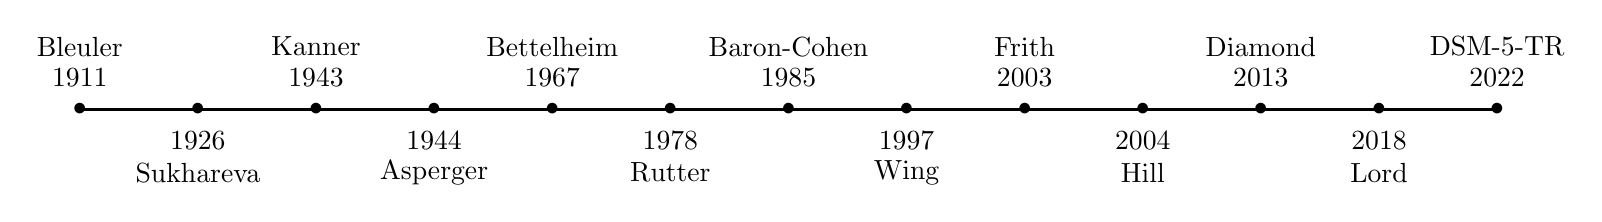
\begin{tikzpicture}

\draw[thick] (0,0) -- (18,0);

% ---------- FILA SUPERIOR ----------

\node at (0,0) {$\bullet$};
\node at (0,0.8) {Bleuler};
\node at (0,0.4) {1911};

\node at (3,0) {$\bullet$};
\node at (3,0.8) {Kanner};
\node at (3,0.4) {1943};

\node at (6,0) {$\bullet$};
\node at (6,0.8) {Bettelheim};
\node at (6,0.4) {1967};

\node at (9,0) {$\bullet$};
\node at (9,0.8) {Baron-Cohen};
\node at (9,0.4) {1985};

\node at (12,0) {$\bullet$};
\node at (12,0.8) {Frith};
\node at (12,0.4) {2003};

\node at (15,0) {$\bullet$};
\node at (15,0.8) {Diamond};
\node at (15,0.4) {2013};

\node at (18,0) {$\bullet$};
\node at (18,0.8) {DSM-5-TR};
\node at (18,0.4) {2022};


% ---------- FILA INFERIOR ----------

\node at (1.5,0) {$\bullet$};
\node at (1.5,-0.8) {Sukhareva};
\node at (1.5,-0.4) {1926};

\node at (4.5,0) {$\bullet$};
\node at (4.5,-0.8) {Asperger};
\node at (4.5,-0.4) {1944};

\node at (7.5,0) {$\bullet$};
\node at (7.5,-0.8) {Rutter};
\node at (7.5,-0.4) {1978};

\node at (10.5,0) {$\bullet$};
\node at (10.5,-0.8) {Wing};
\node at (10.5,-0.4) {1997};

\node at (13.5,0) {$\bullet$};
\node at (13.5,-0.8) {Hill};
\node at (13.5,-0.4) {2004};

\node at (16.5,0) {$\bullet$};
\node at (16.5,-0.8) {Lord};
\node at (16.5,-0.4) {2018};

\end{tikzpicture}

}

\caption{Evolución histórica del concepto de autismo}
\end{figure}



\begin{table}[H]
\centering
\begin{tabular}{|c|c|p{7.5cm}|}
\hline

Año & Autor & Aporte principal \\

\hline

1911 & Bleuler & Introduce el término \textit{autismus} para describir el repliegue hacia la vida interior en pacientes con esquizofrenia. \\

1926 & Sukhareva & Describe por primera vez casos infantiles con características similares al autismo actual. \\

1943 & Kanner & Define el autismo infantil temprano como un síndrome distinto. \\

1944 & Asperger & Describe niños con dificultades sociales pero con lenguaje y cognición preservados. \\

1967 & Bettelheim & Populariza la teoría de la “madre nevera”, atribuyendo el autismo a una crianza emocionalmente fría (hipótesis posteriormente refutada). \\

1978 & Rutter & Propone que el autismo es un trastorno del desarrollo con base biológica. \\

1985 & Baron-Cohen & Desarrolla la teoría de la mente aplicada al autismo. \\

1997 & Wing & Introduce el concepto de espectro autista y la tríada de alteraciones. \\

2003 & Frith & Explica el autismo desde la cognición social y el procesamiento mental. \\

2004 & Hill & Relaciona el autismo con funciones ejecutivas y control cognitivo. \\

2013 & Diamond & Describe el control inhibitorio como función ejecutiva clave. \\

2018 & Lord & Define el autismo desde el modelo moderno del neurodesarrollo. \\

2022 & APA & Publicación del DSM-5-TR con la definición actual del Trastorno del Espectro Autista. \\

\hline

\end{tabular}

\caption{Autores y aportes principales en la evolución del concepto de autismo}
\end{table}






\subsection{Definición del concepto}

El Trastorno del Espectro Autista (TEA) se define actualmente como una condición del neurodesarrollo, es decir, como una forma particular en la que el cerebro se organiza y funciona desde las primeras etapas de la vida. Este enfoque se ha consolidado progresivamente a lo largo de la historia de la investigación sobre el autismo, pasando de interpretaciones clínicas limitadas a modelos más amplios basados en la psicología del desarrollo, la neurociencia y la genética. En la actualidad, la referencia principal para la definición diagnóstica es el \textit{Diagnostic and Statistical Manual of Mental Disorders, Fifth Edition, Text Revision} (DSM-5-TR), manual publicado por la American Psychiatric Association y utilizado internacionalmente para la clasificación de los trastornos mentales. Según este manual, el Trastorno del Espectro Autista se caracteriza por dificultades persistentes en la comunicación social y en la interacción, junto con patrones restrictivos y repetitivos de comportamiento, intereses o actividades, los cuales se manifiestan desde etapas tempranas del desarrollo y afectan el funcionamiento cotidiano en distintos contextos \cite{APA2022, Lord2018, Hirota2023}.

La definición actual es el resultado de varios cambios conceptuales ocurridos durante la segunda mitad del siglo XX. Investigaciones como las de Rutter demostraron que el autismo debía entenderse como un trastorno del desarrollo con bases biológicas, alejándose de explicaciones centradas exclusivamente en factores ambientales. Posteriormente, Wing propuso el concepto de espectro autista, señalando que las características podían presentarse con distintos niveles de intensidad y combinaciones diversas, lo que permitió comprender que no existe un único tipo de autismo, sino múltiples formas de manifestarse. A estos aportes se sumaron los modelos cognitivos de Frith y Baron-Cohen, quienes estudiaron procesos como la teoría de la mente, la cognición social y las funciones ejecutivas, contribuyendo a explicar por qué las personas dentro del espectro pueden mostrar diferencias en la comprensión social, la flexibilidad cognitiva y el control del comportamiento \cite{Wing1997, Frith2003, BaronCohen2000, Hill2004}.

Desde esta perspectiva, el autismo no se considera una enfermedad que aparece de manera repentina, sino una trayectoria de desarrollo distinta que acompaña a la persona a lo largo de la vida. La variabilidad es una de sus características principales: algunas personas requieren altos niveles de apoyo para la vida diaria, mientras que otras pueden desenvolverse con mayor autonomía, aunque continúen presentando diferencias en la comunicación, la regulación emocional o la adaptación a cambios. Por esta razón, el diagnóstico actual se entiende como un continuo, en el que se reconocen distintos niveles de apoyo necesarios según las características individuales, en lugar de categorías rígidas como ocurría en clasificaciones anteriores \cite{APA2022, Happe2020, Lord2018}.

Las revisiones contemporáneas señalan que esta concepción dimensional del TEA refleja mejor la evidencia científica disponible, la cual muestra que el autismo implica variaciones en múltiples sistemas del desarrollo, incluyendo procesos cognitivos, emocionales y neurobiológicos. Esta comprensión más amplia ha permitido orientar la investigación hacia el estudio de funciones específicas, como el control inhibitorio, la flexibilidad cognitiva y la regulación de la actividad cerebral, aspectos que resultan especialmente relevantes para investigaciones que utilizan técnicas neurofisiológicas como el electroencefalograma, al permitir relacionar el comportamiento observable con la dinámica funcional del cerebro \cite{Happe2020, Lord2018, Hirota2023}.

\subsection{Niveles de autismo (énfasis en TEA nivel 1)}

En la actualidad, el Trastorno del Espectro Autista se clasifica según el nivel de apoyo que necesita la persona para desenvolverse en la vida diaria. Esta clasificación fue establecida en el \textit{Diagnostic and Statistical Manual of Mental Disorders, Fifth Edition, Text Revision} (DSM-5-TR), donde se propone un único diagnóstico dentro del espectro autista con tres niveles de apoyo:
\begin{itemize}
    \item Nivel 1 (requiere apoyo);
    \item Nivel 2 (requiere apoyo sustancial);
    \item Nivel 3 (requiere apoyo muy sustancial).
\end{itemize}
Este cambio reemplazó clasificaciones anteriores que separaban el autismo, el síndrome de Asperger y otros trastornos generalizados del desarrollo, y permitió entender el autismo como un continuo con diferentes formas de manifestarse \cite{APA2022, Lord2018}.\\

El TEA nivel 1 corresponde a personas que pueden comunicarse verbalmente y realizar muchas actividades de manera autónoma, pero que presentan dificultades significativas cuando las situaciones requieren adaptación social, flexibilidad o regulación del comportamiento. Estas personas pueden mantener conversaciones, aprender contenidos académicos y participar en actividades cotidianas, aunque suelen experimentar problemas para comprender normas sociales implícitas, interpretar el contexto emocional de los demás o manejar cambios inesperados. Es importante señalar que el nivel no describe la gravedad del autismo de forma permanente, sino la cantidad de apoyo necesaria en un contexto determinado, la cual puede variar según las exigencias del entorno \cite{APA2022, Happe2020}.

En el contexto escolar, el TEA nivel 1 puede pasar desapercibido durante largos periodos, ya que el estudiante puede mostrar buen rendimiento académico en tareas estructuradas, como leer, escribir o resolver ejercicios, pero presentar dificultades cuando se le exige organización, planificación o adaptación a instrucciones cambiantes. Estas situaciones ponen en evidencia alteraciones en funciones ejecutivas, conjunto de procesos cognitivos que permiten regular la conducta, controlar impulsos, mantener la atención y ajustar las acciones a los objetivos. Diversos estudios han encontrado que las personas dentro del espectro, especialmente en niveles de apoyo más bajos, pueden presentar dificultades en la flexibilidad cognitiva, el control inhibitorio y la planificación, lo que afecta su desempeño en actividades escolares que requieren autorregulación y toma de decisiones \cite{Hill2004, Geurts2009, Diamond2013}.

Las investigaciones sobre funciones ejecutivas en autismo señalan que estas dificultades no siempre se observan en tareas simples, sino que aparecen cuando la actividad exige cambiar de estrategia, inhibir respuestas automáticas o adaptarse a reglas nuevas. Por esta razón, el estudio del control inhibitorio y de la regulación del comportamiento resulta especialmente relevante para comprender el funcionamiento cognitivo en el TEA nivel 1, ya que permite analizar cómo el cerebro responde ante situaciones que requieren detener una acción, elegir entre varias opciones o mantener la atención frente a estímulos distractores. Este enfoque ha sido ampliamente utilizado en investigaciones neuropsicológicas y neurofisiológicas, donde técnicas como el electroencefalograma permiten observar la actividad cerebral asociada a estos procesos y relacionarla con el desempeño conductual \cite{Diamond2013, Hill2004, Lord2018}.

\subsection{Autismo y desarrollo cerebral}

El Trastorno del Espectro Autista se considera actualmente una condición del neurodesarrollo, lo que implica que sus características están relacionadas con la forma en que el cerebro se organiza y madura desde las primeras etapas de la vida. Las investigaciones en neurociencia han mostrado que en el TEA no existe una lesión única ni una alteración localizada específica, sino patrones de desarrollo cerebral diferentes que afectan la conectividad, la sincronización y el equilibrio funcional entre distintas regiones del sistema nervioso \cite{Courchesne2007, Ecker2015, Lord2018}.


\begin{figure}[H]
\centering
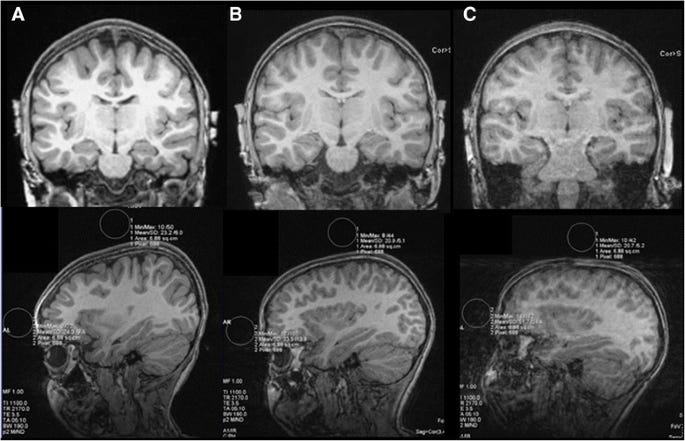
\includegraphics[width=0.8\textwidth]{autismo3.jpg}
\caption{Descripción clara y académica de la imagen.}
\label{fig:ejemplo}
\end{figure}



Estudios de neuroimagen estructural y funcional han encontrado variaciones en el crecimiento temprano del cerebro, especialmente en regiones frontales, temporales y en el sistema límbico, áreas asociadas con la regulación de la conducta, la interacción social, la planificación y el control emocional. Courchesne (2007) describe que en muchos casos se observa un crecimiento cerebral acelerado en la infancia temprana, seguido de trayectorias de desarrollo atípicas, lo que puede influir en la manera en que se integran los procesos cognitivos y emocionales \cite{Courchesne2007}. De manera complementaria, investigaciones posteriores han señalado diferencias en la conectividad funcional, es decir, en la forma en que distintas regiones cerebrales se comunican entre sí durante la realización de tareas cognitivas \cite{Ecker2015, Just2012}.

Estas variaciones no deben interpretarse como un déficit global, sino como una organización neurobiológica distinta, que puede favorecer ciertos tipos de procesamiento y dificultar otros. Por ejemplo, se ha observado que algunas personas con TEA muestran mayor actividad en circuitos relacionados con el procesamiento perceptivo detallado, mientras que presentan menor integración en redes encargadas de la regulación y el control ejecutivo \cite{Frith2003, Uddin2013}. Esta diferencia en la organización cerebral puede explicar por qué, en situaciones que requieren flexibilidad, planificación o control de impulsos, el desempeño puede verse afectado aun cuando la capacidad intelectual general se mantenga dentro del promedio.

Las regiones prefrontales, especialmente la corteza prefrontal dorsolateral y orbitofrontal, cumplen un papel fundamental en la regulación del comportamiento, el control inhibitorio y la toma de decisiones. Diversos estudios han señalado que las diferencias en la maduración de estos sistemas pueden estar relacionadas con las dificultades para detener respuestas automáticas, cambiar de estrategia o mantener la conducta orientada a una meta, procesos que forman parte de las funciones ejecutivas \cite{Diamond2013, Hill2004}. Estas características suelen hacerse más evidentes en contextos escolares o en tareas complejas, donde se requiere coordinar múltiples procesos cognitivos al mismo tiempo.

Debido a que estas funciones dependen de la actividad coordinada de redes neuronales distribuidas, el estudio del TEA ha incorporado técnicas que permiten observar el funcionamiento cerebral en tiempo real. Entre ellas, el electroencefalograma (EEG) se ha convertido en una herramienta relevante, ya que permite analizar la actividad eléctrica cortical durante la realización de tareas cognitivas y conductuales. El uso del EEG ha facilitado la identificación de patrones de activación asociados con la atención, la regulación y el control inhibitorio, lo que ha contribuido a comprender cómo las diferencias en el desarrollo cerebral pueden manifestarse en el desempeño cognitivo \cite{Uhlhaas2006, Luck2014}.

En conjunto, la evidencia sugiere que el autismo debe entenderse como una variación en la organización del sistema nervioso que afecta la integración entre procesos emocionales, cognitivos y conductuales. Esta perspectiva resulta fundamental para analizar posteriormente el desarrollo cognitivo, las funciones ejecutivas y el control inhibitorio, así como para justificar el uso de técnicas neurofisiológicas como el EEG en el estudio del funcionamiento mental en personas con TEA.

% 1 -> INCIO CAP REVISIÓN
\subsection{El cerebro humano: regiones y su relación con las señales EEG}

El cerebro humano es el órgano más complejo del sistema nervioso central y constituye la base biológica de todos los procesos cognitivos, emocionales y conductuales que se estudian en esta investigación. Desde el punto de vista anatómico, el cerebro se organiza en cuatro lóbulos principales que presentan especializaciones funcionales diferenciadas, aunque operan de manera integrada a través de redes de conectividad distribuidas \cite{Kandel2000, Bear2016}.

\begin{itemize}
    \item \textbf{Lóbulo frontal:} funciones ejecutivas y control del comportamiento.
    \item \textbf{Lóbulo parietal:} integración sensorial y atención espacial.
    \item \textbf{Lóbulo occipital:} procesamiento visual.
    \item \textbf{Lóbulo temporal:} memoria, lenguaje y emoción.
\end{itemize}

\begin{figure}[h]
    \centering
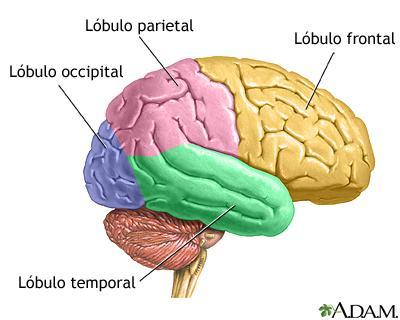
\includegraphics[width=0.45\textwidth]{lobulos_cerebro.jpg}
    \caption{Estructura de los lóbulos cerebrales. Fuente: \protect\cite{cenie_lobulo}}
    \label{fig:lobulos}
\end{figure}
\subsubsection*{Lóbulo frontal}

El lóbulo frontal ocupa la región anterior del cerebro y contiene la corteza motora primaria, responsable del control voluntario del movimiento, y la corteza prefrontal, que constituye el sustrato neural de las funciones ejecutivas.

\begin{itemize}
    \item \textbf{Corteza prefrontal dorsolateral:} planificación, memoria de trabajo y control inhibitorio.
    \item \textbf{Corteza orbitofrontal:} toma de decisiones y regulación emocional.
\end{itemize}

Las investigaciones en neuroimagen han demostrado que la actividad del lóbulo frontal, medida a través del electroencefalograma, se relaciona directamente con el nivel de demanda cognitiva de una tarea: cuando las regiones prefrontales son reclutadas activamente, se observa una reducción en la potencia de las oscilaciones alfa, fenómeno conocido como \textit{desincronización alfa} \cite{Klimesch1999, Pfurtscheller1999}.

En el contexto del Trastorno del Espectro Autista de nivel 1, estas dinámicas se asocian con dificultades en:

\begin{itemize}
    \item Control inhibitorio.
    \item Flexibilidad cognitiva.
    \item Planificación secuencial.
\end{itemize}

\subsubsection*{Lóbulo parietal}

El lóbulo parietal se localiza en la región superior y posterior del cerebro y contiene la corteza somatosensorial primaria, encargada de procesar la información táctil y propioceptiva.

\begin{itemize}
    \item Integración multisensorial.
    \item Atención espacial.
    \item Coordinación percepción–acción.
\end{itemize}

En el análisis EEG, los electrodos parietales del sistema 10-20 (P3, Pz, P4) funcionan como indicadores de procesamiento atencional.

\textbf{Interpretación de la banda alfa parietal:}
\begin{itemize}
    \item Alta potencia alfa $\rightarrow$ menor activación atencional.
    \item Supresión alfa $\rightarrow$ procesamiento activo.
\end{itemize}

\subsubsection*{Lóbulo occipital}

El lóbulo occipital alberga la corteza visual primaria y áreas de asociación visual.

\begin{itemize}
    \item Procesamiento de contraste, orientación y movimiento.
    \item Reconocimiento de objetos.
    \item Percepción del color.
\end{itemize}

En el EEG, los electrodos O1, Oz y O2 capturan actividad visual. El ritmo alfa occipital (ritmo de Berger) es prominente en reposo y se suprime durante el procesamiento visual activo \cite{Klimesch1999}.

\begin{figure}[H]
\centering
\fbox{\parbox{0.8\textwidth}{
\textcolor{red}{Aquí agregar una imagen de un montaje EEG destacando electrodos occipitales O1, Oz y O2}
}}
\caption{Ubicación de electrodos occipitales en el sistema 10-20.}
\label{fig:electrodos_occipitales}
\end{figure}

\subsubsection*{Lóbulo temporal}

El lóbulo temporal contiene estructuras clave, como el hipocampo y la amígdala.

\begin{itemize}
    \item \textbf{Hipocampo:} memoria y aprendizaje.
    \item \textbf{Amígdala:} procesamiento emocional.
\end{itemize}

En EEG, los electrodos T7, T8, TP9 y TP10 reflejan procesos de:

\begin{itemize}
    \item Lenguaje.
    \item Memoria.
    \item Regulación emocional.
\end{itemize}

En el TEA, las diferencias en conectividad temporal se relacionan con variaciones en:

\begin{itemize}
    \item Procesamiento social.
    \item Regulación emocional.
\end{itemize}

\subsubsection*{Importancia de la distribución regional para el análisis EEG}

La especialización funcional de los lóbulos cerebrales fundamenta el análisis topográfico del EEG.

\begin{itemize}
    \item Cada canal refleja actividad cortical subyacente.
    \item Permite construir mapas de activación.
    \item Facilita la interpretación funcional durante tareas cognitivas.
\end{itemize}

En esta investigación, el análisis de la potencia relativa alfa permite integrar:

\begin{itemize}
    \item Región frontal $\rightarrow$ control ejecutivo.
    \item Región parietal $\rightarrow$ atención.
    \item Región temporal $\rightarrow$ memoria/emoción.
    \item Región occipital $\rightarrow$ procesamiento visual.
\end{itemize}

\begin{figure}[H]
\centering
\fbox{\parbox{0.8\textwidth}{
\textcolor{red}{Aquí agregar una imagen de mapa topográfico EEG (topoplot) mostrando distribución de actividad cerebral}
}}
\caption{Ejemplo de mapa topográfico de actividad EEG.}
\label{fig:topoplot_eeg}
\end{figure}

\subsection{Registro electroencefalográfico: electrodos, sistemas de posicionamiento y el Ultracortex Mark IV}

El registro electroencefalográfico requiere la colocación precisa de electrodos sobre el cuero cabelludo para capturar la actividad eléctrica cortical.

\textbf{Factores que determinan la calidad del registro:}
\begin{itemize}
    \item Número de electrodos.
    \item Posición en el cuero cabelludo.
    \item Tipo de electrodo.
    \item Impedancia electrodo-piel.
\end{itemize}

\subsubsection*{Sistemas de posicionamiento de electrodos}

El sistema internacional 10-20 garantiza estandarización y reproducibilidad.

\begin{itemize}
    \item Basado en proporciones del cráneo (10\% y 20\%).
    \item Nomenclatura:
    \begin{itemize}
        \item Letras: región (F, C, P, O, T).
        \item Números: lateralidad (impar = izquierda, par = derecha).
        \item z: línea media.
    \end{itemize}
\end{itemize}

\begin{figure}[H]
\centering
\fbox{\parbox{0.8\textwidth}{
\textcolor{red}{Aquí agregar una imagen del sistema internacional 10-20 con etiquetas}
}}
\caption{Sistema internacional 10-20 para posicionamiento de electrodos.}
\label{fig:sistema_1020}
\end{figure}

\subsubsection*{Tipos de electrodos para EEG}

\begin{itemize}
    \item \textbf{Húmedos:} alta calidad de señal, requieren gel.
    \item \textbf{Activos:} menor ruido, amplificación integrada.
    \item \textbf{Secos:} rápida instalación, mayor ruido.
\end{itemize}

\subsubsection*{El Ultracortex Mark IV de OpenBCI}

El Ultracortex Mark IV es un casco EEG modular de código abierto diseñado para investigación y educación.

\textbf{Características principales:}
\begin{itemize}
    \item Diseño ajustable e imprimible en 3D.
    \item 16 electrodos (configuración usada en el estudio).
    \item Compatible con sistema 10-20.
\end{itemize}

\begin{figure}[H]
\centering
\fbox{\parbox{0.8\textwidth}{
\textcolor{red}{Aquí agregar imagen del casco Ultracortex Mark IV con electrodos montados}
}}
\caption{Casco Ultracortex Mark IV con distribución de electrodos.}
\label{fig:ultracortex}
\end{figure}

\textbf{Distribución de electrodos utilizada:}
\begin{itemize}
    \item Frontales: Fp1, Fp2, F3, F4, F7, F8
    \item Centrales: C3, C4
    \item Temporales: T7, T8
    \item Parietales: P3, P4, P7, P8
    \item Occipitales: O1, O2
\end{itemize}

\subsubsection*{De la señal EEG a las frecuencias de ondas cerebrales}

El análisis espectral permite descomponer la señal EEG en bandas de frecuencia.

\begin{itemize}
    \item \textbf{Delta (0.5--4 Hz):} sueño profundo.
    \item \textbf{Theta (4--8 Hz):} memoria de trabajo.
    \item \textbf{Alfa (8--13 Hz):} inhibición/activación cortical.
    \item \textbf{Beta (13--30 Hz):} alerta cognitiva.
    \item \textbf{Gamma (30--100 Hz):} integración cognitiva.
\end{itemize}

\begin{figure}[H]
\centering
\fbox{\parbox{0.8\textwidth}{
\textcolor{red}{Aquí agregar una imagen del espectro de frecuencias EEG mostrando las bandas}
}}
\caption{Bandas de frecuencia en el electroencefalograma.}
\label{fig:bandas_eeg}
\end{figure}

\subsubsection*{Postprocesamiento en MATLAB y obtención del Alpha TRP}

El procesamiento se realiza en MATLAB con EEGLAB \cite{Delorme2004}.

\textbf{Flujo de procesamiento:}
\begin{enumerate}
    \item Importación de datos.
    \item Configuración de canales.
    \item Filtrado (1–40 Hz + notch 60 Hz).
    \item Inspección e interpolación de artefactos.
\end{enumerate}

\textbf{Cálculo del Alpha TRP:}
\begin{itemize}
    \item Aplicación de la FFT (Transformada Rápida de Fourier).
    \item Cálculo de la potencia relativa:
\end{itemize}

\begin{center}
\textbf{Alpha TRP = Potencia en banda alfa / Potencia total (1–40 Hz)}
\end{center}

\begin{figure}[H]
\centering
\fbox{\parbox{0.8\textwidth}{
\textcolor{red}{Aquí agregar una imagen de una gráfica de espectro de potencia EEG en MATLAB}
}}
\caption{Espectro de potencia EEG obtenido mediante FFT.}
\label{fig:fft_eeg}
\end{figure}

Este procedimiento permite generar mapas topográficos que representan la activación cortical durante la tarea.

La comparación entre sesiones (con y sin mediación) constituye el núcleo analítico del estudio, permitiendo identificar patrones de:

\begin{itemize}
    \item Impulsividad.
    \item Planificación.
    \item Toma de decisiones.
\end{itemize}

Este enfoque, de carácter exploratorio, busca identificar tendencias que orienten investigaciones futuras con mayor escala experimental \cite{Luck2014, Klimesch1999, Delorme2004}.
% 2-> FINN



\subsection{Autismo y desarrollo cognitivo}

Desde el punto de vista cognitivo, el Trastorno del Espectro Autista se asocia con un patrón particular de procesamiento de la información que no implica necesariamente una menor capacidad intelectual, sino una forma diferente de percibir, organizar e interpretar los estímulos del entorno. Diversos estudios han mostrado que muchas personas con TEA, especialmente en el nivel 1, pueden presentar inteligencia dentro del promedio o superior, pero manifiestan diferencias en la forma en que integran la información y se adaptan a situaciones cambiantes \cite{Frith2003, Happe2020, Hill2004}.

Uno de los modelos más influyentes para explicar estas características es la teoría de la coherencia central débil, propuesta por Frith, según la cual las personas con autismo tienden a centrarse en los detalles más que en la idea global. Este estilo cognitivo puede favorecer el rendimiento en tareas estructuradas o repetitivas, pero generar dificultades cuando la actividad requiere comprender el contexto completo o relacionar múltiples elementos al mismo tiempo \cite{Frith2003, Happe2006}.

Otro enfoque relevante es la teoría de la mente, desarrollada por Baron-Cohen, que describe la capacidad de comprender los pensamientos, emociones e intenciones de otras personas. Las investigaciones han mostrado que en el TEA pueden existir diferencias en este tipo de procesamiento social, lo que influye en la interacción y en la interpretación de situaciones que no siguen reglas explícitas \cite{BaronCohen2000}.

Además, estudios en neuropsicología han señalado que el rendimiento cognitivo en el autismo puede variar según la complejidad de la tarea y la cantidad de información que debe mantenerse activa durante su ejecución. En actividades que requieren organizar varios pasos, mantener la atención o adaptarse a cambios, pueden aparecer dificultades que no se observan en tareas simples o altamente estructuradas \cite{Baddeley2000, Williams2006}.

Estas características han llevado a que la investigación actual preste especial atención a los procesos de regulación cognitiva que permiten dirigir la conducta hacia una meta, mantener la información relevante y evitar respuestas impulsivas. Dichos procesos forman parte de las llamadas funciones ejecutivas, las cuales serán abordadas en la siguiente sección debido a su importancia para comprender el funcionamiento cognitivo en el Trastorno del Espectro Autista.


\subsection{Funciones ejecutivas en el TEA}

Las funciones ejecutivas constituyen un sistema de procesos 
cognitivos de alto nivel que permite regular el pensamiento 
y la conducta con el fin de alcanzar objetivos. Diamond 
propone que este sistema está organizado en tres componentes 
fundamentales e interrelacionados: la memoria de trabajo, 
que permite mantener y manipular información relevante 
mientras se ejecuta una tarea; la flexibilidad cognitiva, 
que permite cambiar de perspectiva o de estrategia cuando 
las condiciones lo requieren; y el control inhibitorio, 
que permite suprimir respuestas automáticas o impulsivas 
para actuar de manera deliberada y orientada a una meta 
\cite{Diamond2013}. Estos tres componentes no operan de 
manera aislada: el control inhibitorio es el mecanismo 
más básico del sistema, ya que sin la capacidad de suprimir 
la respuesta dominante, tanto el mantenimiento de 
información en memoria de trabajo como el cambio de 
estrategia se ven comprometidos \cite{Diamond2013, Miyake2000}.

El modelo de Miyake y colaboradores complementa esta 
visión al describir las funciones ejecutivas como un 
sistema compuesto por componentes distinguibles pero 
correlacionados, cuya coordinación permite que la persona 
mantenga la información relevante, inhiba respuestas 
automáticas y ajuste su conducta cuando la situación lo 
requiere \cite{Miyake2000}. Desde el punto de vista 
neuropsicológico, estos procesos dependen principalmente 
de la actividad de la corteza prefrontal y de sus 
conexiones con regiones corticales y subcorticales, lo 
que explica su papel en la regulación voluntaria del 
comportamiento y en la toma de decisiones.

En el Trastorno del Espectro Autista, numerosos estudios han identificado diferencias en el funcionamiento de las funciones ejecutivas, especialmente en tareas que requieren planificación, cambio de reglas o control de respuestas 
impulsivas. Hill realizó una revisión sistemática de la evidencia disponible y encontró que las dificultades ejecutivas en el TEA no se manifiestan de manera uniforme en todas las tareas: son más evidentes cuando la actividad 
exige organizar varios pasos en secuencia, mantener activa la meta mientras se ejecutan submetas intermedias, o adaptarse a condiciones que cambian durante la tarea 

\cite{Hill2004}. Geurts y colaboradores, en un estudio 
comparativo con grupos de diferente edad y nivel de 
funcionamiento, encontraron que las personas con TEA 
muestran rendimiento adecuado en tareas simples de 
inhibición, pero presentan mayor variabilidad y mayor 
tasa de errores cuando la tarea exige inhibición bajo 
interferencia emocional o alta carga cognitiva simultánea 
\cite{Geurts2009}. Esta distinción entre inhibición 
simple e inhibición bajo demanda compleja es especialmente 
relevante para el TEA nivel 1, donde las dificultades 
ejecutivas pueden pasar desapercibidas en evaluaciones 
estándar pero se hacen visibles en contextos de aprendizaje 
que requieren autorregulación sostenida.

La relación entre funciones ejecutivas y desempeño 
académico ha sido ampliamente documentada. En tareas de 
resolución de problemas matemáticos, el aprendiz debe 
coordinar simultáneamente la memoria de trabajo para 
retener los pasos ya ejecutados, la flexibilidad cognitiva 
para revisar una estrategia que no está funcionando, y 
el control inhibitorio para resistir la tentación de 
ejecutar el movimiento más inmediato y aparentemente 
sencillo en lugar del más eficiente a largo plazo 
\cite{Diamond2013, Baddeley2000}. Esta coordinación 
resulta especialmente demandante en tareas de 
transformación como el juego La Escalera, donde cada 
decisión modifica el espacio de estados disponibles para 
las decisiones siguientes, y donde un movimiento impulsivo 
puede cerrar caminos de solución que son difíciles de 
recuperar sin retroceder.

Dentro del sistema de funciones ejecutivas, el control 
inhibitorio ocupa una posición central tanto teórica como 
funcionalmente. Diamond señala que la capacidad de inhibir 
constituye el punto de partida del control ejecutivo 
voluntario, ya que permite crear el espacio cognitivo 
necesario para que operen la planificación y la 
flexibilidad \cite{Diamond2013}. Por esta razón, el 
análisis del control inhibitorio en estudiantes con TEA 
nivel 1 durante la resolución de una tarea estructurada 
permite observar de manera directa el funcionamiento del 
sistema ejecutivo en condiciones de demanda cognitiva 
real, complementando la información conductual con el 
registro de la actividad cerebral mediante técnicas 
neurofisiológicas.



\subsection{Autismo y control inhibitorio}

El control inhibitorio es uno de los componentes fundamentales de las funciones ejecutivas y se refiere a la capacidad de suprimir respuestas automáticas, resistir distracciones y regular la conducta con el fin de actuar de manera adecuada según las demandas de la situación. Este proceso permite detener una acción impulsiva, esperar el momento adecuado para responder y mantener el comportamiento orientado hacia una meta, lo que resulta esencial en el aprendizaje, la toma de decisiones y la resolución de problemas \cite{Diamond2013, Miyake2000}.

Desde el punto de vista neuropsicológico, el control inhibitorio depende principalmente de la actividad de la corteza prefrontal y de su interacción con otras regiones cerebrales involucradas en la regulación emocional y el control motor. Barkley señala que la inhibición conductual constituye un mecanismo central para el funcionamiento ejecutivo, ya que permite organizar la conducta en el tiempo, anticipar consecuencias y ajustar la respuesta antes de actuar \cite{Barkley1997}. Cuando este proceso se ve afectado, pueden aparecer dificultades para seguir reglas, mantener la atención o evitar respuestas impulsivas.

En el Trastorno del Espectro Autista, diversos estudios han encontrado diferencias en el desempeño en tareas que requieren control inhibitorio, especialmente cuando la actividad implica cambiar de estrategia, ignorar estímulos irrelevantes o detener una respuesta previamente aprendida. Hill indica que estas dificultades suelen hacerse más evidentes en tareas complejas, donde se requiere coordinar varios procesos cognitivos al mismo tiempo, lo que sugiere que el problema no se limita a una habilidad específica, sino a la regulación general del comportamiento \cite{Hill2004}. De manera similar, Geurts y colaboradores encontraron que las personas con TEA pueden presentar un rendimiento adecuado en tareas simples, pero mostrar mayor variabilidad cuando la situación exige flexibilidad y control voluntario de la respuesta \cite{Geurts2009}.

El control inhibitorio también está relacionado con la regulación emocional. Cuando una persona experimenta frustración, ansiedad o sobrecarga cognitiva, la capacidad para detener una respuesta automática puede disminuir, lo que afecta el desempeño en tareas académicas o en situaciones que requieren concentración sostenida. Este aspecto resulta especialmente relevante en contextos educativos, donde la resolución de problemas no depende únicamente del conocimiento, sino también de la capacidad para controlar la conducta y mantener la atención en la meta \cite{Diamond2013}.

Debido a su papel en la regulación del comportamiento y en el funcionamiento cognitivo, el estudio del control inhibitorio se ha convertido en un área de interés en la investigación sobre autismo. En particular, el uso de técnicas neurofisiológicas ha permitido analizar cómo se activan las redes cerebrales durante tareas que requieren inhibir respuestas, lo que ha contribuido a comprender mejor la relación entre la actividad cerebral y el desempeño conductual. Por esta razón, en la siguiente sección se revisan los avances en investigación que utilizan el electroencefalograma como herramienta para estudiar estos procesos.

\subsection{Regulación emocional en el TEA}

La regulación emocional se refiere a la capacidad de modificar, controlar o ajustar las propias emociones con el fin de responder de manera adecuada a las demandas del entorno. Este proceso implica reconocer los estados emocionales, inhibir reacciones impulsivas y utilizar estrategias cognitivas para mantener la conducta orientada hacia un objetivo. Desde el punto de vista neuropsicológico, la regulación emocional depende de la interacción entre la corteza prefrontal y el sistema límbico, especialmente la amígdala, estructuras que participan en la evaluación de los estímulos y en el control de la respuesta emocional \cite{Gross1998, Uddin2013}.

En el Trastorno del Espectro Autista, diversos estudios han señalado que pueden presentarse diferencias en la forma en que se procesan y regulan las emociones. Estas diferencias no implican ausencia de respuesta emocional, sino variaciones en los mecanismos que permiten modular la intensidad de la reacción, adaptarse a situaciones nuevas o manejar la frustración. Investigaciones recientes han mostrado que las dificultades en la regulación emocional pueden estar relacionadas con alteraciones en la conectividad entre regiones frontales y límbicas, lo que afecta la capacidad para controlar la conducta en contextos que requieren flexibilidad y adaptación \cite{Mazefsky2013, Uddin2013}.

La regulación emocional está estrechamente relacionada con las funciones ejecutivas, ya que controlar una emoción implica inhibir respuestas automáticas, mantener la atención en la tarea y seleccionar estrategias adecuadas para resolver un problema. Diamond señala que el control inhibitorio constituye uno de los mecanismos básicos que permiten regular tanto la conducta como la respuesta emocional, por lo que las dificultades en este proceso pueden influir directamente en el desempeño cognitivo \cite{Diamond2013}. En el contexto escolar, estas dificultades pueden manifestarse cuando el estudiante se enfrenta a tareas complejas, errores inesperados o situaciones que generan presión, lo que puede afectar la concentración y la toma de decisiones.

En personas con TEA, la regulación emocional adquiere especial relevancia debido a que muchas actividades académicas requieren mantener el control de la conducta durante periodos prolongados, tolerar la frustración y adaptarse a cambios en la tarea. Estudios en neurociencia han señalado que las diferencias en la activación de redes frontales durante situaciones de demanda cognitiva pueden estar asociadas con variaciones en el control emocional y en la capacidad para mantener la meta de la actividad \cite{Lord2018, Samson2014}. Estas observaciones han llevado a que la investigación actual explore la relación entre regulación emocional, control inhibitorio y actividad cerebral mediante técnicas neurofisiológicas.

Debido a que la regulación emocional involucra procesos cognitivos y neuronales que pueden analizarse en tiempo real, el uso de técnicas como el electroencefalograma ha permitido estudiar cómo se activan las redes cerebrales durante tareas que requieren controlar la conducta y manejar la frustración. Por esta razón, la investigación con EEG se ha convertido en una herramienta relevante para comprender la relación entre actividad cerebral, control inhibitorio y desempeño cognitivo en personas con Trastorno del Espectro Autista.


\subsection{Avances en investigación con EEG y control 
inhibitorio en el TEA}

El electroencefalograma (EEG) es una técnica de registro 
neurofisiológico que mide la actividad eléctrica cortical 
mediante electrodos colocados sobre el cuero cabelludo. 
Su principal ventaja frente a otras técnicas de neuroimagen 
es su alta resolución temporal: permite observar cambios 
en la actividad neuronal en escalas de milisegundos, lo 
que resulta especialmente útil para estudiar procesos 
cognitivos que ocurren de manera rápida y dinámica durante 
la ejecución de una tarea \cite{Luck2014}. Esta 
característica convierte al EEG en una herramienta 
adecuada tanto para paradigmas experimentales discretos, 
en los que se analiza la respuesta cerebral ante estímulos 
específicos, como para el registro continuo de la actividad 
durante tareas naturales o semiestructuradas de mayor 
duración \cite{Uhlhaas2006}.

En la investigación sobre control inhibitorio, el EEG 
ha sido ampliamente utilizado mediante dos aproximaciones 
complementarias. La primera es el análisis de potenciales 
relacionados con eventos (ERP), que permite identificar 
componentes específicos de la respuesta cerebral asociados 
con procesos de inhibición y monitoreo. Entre los más 
estudiados en tareas de control inhibitorio se encuentran 
el componente N200, una deflexión negativa que aparece 
entre 200 y 350 milisegundos después del estímulo y 
que refleja el proceso activo de supresión de una 
respuesta prepotente; el P300, una deflexión positiva 
que ocurre entre 300 y 600 milisegundos y que se asocia 
con la evaluación del estímulo y la actualización del 
contexto en la memoria de trabajo; y el error-related 
negativity (ERN), que aparece inmediatamente después 
de la comisión de un error y refleja el monitoreo del 
desempeño y la detección de conflicto \cite{Luck2014, 
Falkenstein2000, Kopp1996}. La segunda aproximación 
es el análisis espectral de la señal, que examina la 
distribución de potencia en bandas de frecuencia durante 
periodos sostenidos de actividad y permite observar el 
estado funcional de las redes neuronales a lo largo de 
una tarea completa, sin requerir la repetición de eventos 
discretos idénticos \cite{Klimesch1999}.

En el estudio del Trastorno del Espectro Autista, ambas 
aproximaciones han contribuido a caracterizar las 
diferencias en el funcionamiento de los sistemas de 
control ejecutivo. Coben y colaboradores analizaron 
patrones de conectividad EEG en personas con TEA y 
encontraron diferencias en la coherencia entre regiones 
frontales y posteriores, lo que sugiere una menor 
integración funcional entre los sistemas de control 
ejecutivo y los sistemas de procesamiento perceptivo 
\cite{Coben2008}. Uhlhaas y Singer, en una revisión 
de la evidencia sobre sincronización neuronal en el 
TEA, identificaron alteraciones en la coordinación 
temporal entre regiones cerebrales durante tareas 
cognitivas, con implicaciones directas para la 
comprensión de cómo se organizan los procesos de 
atención y regulación en el espectro \cite{Uhlhaas2006}. 
Kana y colaboradores registraron actividad EEG durante 
tareas de inhibición en personas con TEA y observaron 
menor activación en regiones frontales asociadas con 
el control de la respuesta, junto con patrones de 
mayor latencia en los componentes electrofisiológicos 
relacionados con el monitoreo del error, lo que 
sugiere que los mecanismos de detección y corrección 
de la respuesta operan de manera diferente en el 
espectro autista \cite{Kana2011}.

Estos hallazgos adquieren especial relevancia en el 
contexto educativo cuando se analizan en relación con 
tareas que requieren control inhibitorio sostenido. 
En la resolución de problemas matemáticos, el aprendiz 
debe inhibir movimientos impulsivos, mantener activa 
la representación del estado meta y monitorear 
continuamente si su trayectoria de solución se acerca 
o se aleja del objetivo. En estudiantes con TEA nivel 
1, las diferencias en la activación frontal y en la 
conectividad funcional descritas por los estudios 
anteriores pueden traducirse en mayor variabilidad en 
el desempeño, mayor dificultad para detectar y 
corregir errores estratégicos, y menor eficiencia 
en el uso de los recursos atencionales disponibles 
\cite{Geurts2009, Hill2004, Kana2011}.

En la presente investigación, el registro EEG se 
realiza de manera continua durante la sesión completa 
de resolución del juego La Escalera, utilizando un 
casco de 16 electrodos OpenBCI con distribución basada 
en el sistema internacional 10-20. Dado el carácter 
exploratorio del estudio, el análisis se centra en 
la potencia relativa alfa por canal (Alpha TRP), una 
métrica espectral que permite comparar el nivel de 
activación cortical entre sesiones y entre regiones 
cerebrales sin requerir la segmentación en eventos 
discretos. Las gráficas de Alpha TRP por canal y los 
mapas topográficos de activación constituyen el insumo 
principal para la discusión de los resultados, con 
el propósito de identificar patrones de activación 
diferencial que orienten investigaciones posteriores 
con mayor control experimental \cite{Klimesch1999, 
Luck2014, Delorme2004}.


\subsection{Conclusiones}

La revisión presentada en este capítulo construye el argumento 
teórico que sustenta la pregunta de investigación de la 
presente tesis. El punto de partida es el reconocimiento 
del Trastorno del Espectro Autista como una condición del 
neurodesarrollo que implica una organización cerebral 
diferente, no un déficit global de capacidades. En el 
nivel 1, esta organización produce un perfil cognitivo 
en el que muchas habilidades académicas se preservan, 
pero el desempeño se ve afectado en situaciones que 
exigen planificación, flexibilidad y, especialmente, 
control inhibitorio: la capacidad de suprimir la 
respuesta automática para actuar de manera deliberada 
\cite{Diamond2013, Hill2004, Geurts2009}.

El control inhibitorio ocupa una posición central en 
este argumento porque es el componente más básico del 
sistema de funciones ejecutivas: sin él, la planificación 
y la flexibilidad cognitiva no pueden operar de manera 
eficaz. Su estudio en contextos de resolución de 
problemas matemáticos resulta especialmente pertinente 
porque tareas como el juego La Escalera exigen 
exactamente ese tipo de regulación: inhibir el 
movimiento más inmediato disponible en favor de una 
secuencia estratégica más eficiente, mantener activa 
la representación del estado meta durante varios pasos 
intermedios, y detectar y corregir errores sin perder 
el control de la conducta \cite{Diamond2013, 
PaezGonzalez2022}. Las diferencias en este proceso, 
documentadas en la literatura mediante análisis 
conductual y neurofisiológico, no son evidentes en 
tareas simples pero emergen con claridad cuando la 
demanda cognitiva se sostiene en el tiempo y requiere 
coordinación entre múltiples sistemas ejecutivos 
\cite{Geurts2009, Kana2011}.

La propuesta de mediación mediante herramientas con 
agentividad responde directamente a este perfil. 
Los cubos inteligentes, activados por el docente 
según su lectura de la situación del aprendiz, 
ofrecen señales externas de regulación ejecutiva 
en el momento en que el control inhibitorio se 
ve comprometido, sin depender de la interpretación 
de lenguaje verbal ni de señales sociales implícitas, 
dos canales que presentan dificultades específicas 
en el TEA nivel 1 \cite{APA2022, PaezGonzalez2022}. 
Esta mediación distribuida entre el cubo y el 
docente supera las limitaciones de los sistemas 
autónomos previos y se ajusta al ritmo real del 
aprendiz en una tarea semiestructurada.

El electroencefalograma, y en particular el análisis 
de la potencia relativa alfa por canal durante la 
sesión completa, permite observar si esa mediación 
produce diferencias en la activación de las redes 
corticales asociadas con el control ejecutivo. 
Dado que el estudio tiene carácter exploratorio 
y trabaja con dos participantes con TEA nivel 1, 
los resultados no pretenden generalización 
estadística: su aporte es identificar patrones 
de activación diferencial que justifiquen y 
orienten investigaciones posteriores con mayor 
control experimental, mayor tamaño de muestra 
y paradigmas más refinados \cite{Klimesch1999, 
Luck2014}. Lo que este capítulo ha construido 
es la base teórica que hace esa exploración 
inteligible: no se registra el EEG por registrarlo, 
sino porque hay razones neurobiológicas, cognitivas 
y pedagógicas para esperar que la mediación con 
herramientas con agentividad deje una huella en 
la actividad cortical de un aprendiz con TEA 
nivel 1 durante la resolución de un problema 
matemático bien definido.




%\section*{Introducción}
%\section{Síndrome de Trastorno del espectro Autista - TEA nivel 1}
%% Estructuraq
% - Historia del Sindrome [2 párrafos]
% - Definición del concepto [1 párrafo]
% - Niveles de autismo (Énfasis en TEA 1) [2 párrafos]
% - Autismo y Desarrollo Cerebral [2 párrafos]
% - Autismo y Desarrollo Cognitivo [2 párrafos]
% - - Autismo + Control Inhibitorio [2 párrafos]
% - Avances en Investigación con EEG [2 párrafos]
% - Conclusiones [1 párrafo]

%El Trastorno del Espectro Autista (TEA) es un trastorno del neurodesarrollo caracterizado por déficits persistentes en la comunicación social y patrones restrictivos y repetitivos de comportamiento \cite{APA2022}. 

%El TEA Nivel 1, según el DSM-5-TR, corresponde a individuos que requieren apoyo, presentan lenguaje funcional y autonomía básica, pero manifiestan dificultades en flexibilidad cognitiva, regulación emocional y funciones ejecutivas.

%Desde la neuropsicología cognitiva, diversos estudios han identificado alteraciones variables en procesos ejecutivos, particularmente en control inhibitorio y flexibilidad cognitiva \cite{Hill2004, Geurts2009}. Estas diferencias no implican déficit intelectual generalizado, sino perfiles ejecutivos heterogéneos dependientes del contexto y la carga cognitiva.


%\section{Control Inhibitorio}

%El control inhibitorio es un componente central de las funciones ejecutivas y se define como la capacidad de suprimir respuestas automáticas o impulsivas para favorecer conductas orientadas a metas \cite{Diamond2013}.

%En población con TEA niadaasdadasdasdadw

% INICIOOO
%2->Inicio cap agregado para revisión

\chapter{Interpretación trayectorias juego}{Trayectorias de solución del juego La Escalera: lectura e interpretación de los grafos}

\section{El grafo como representación del espacio del problema}

Para comprender la solución del juego La Escalera y analizar el proceso cognitivo de quien lo resuelve, es necesario contar con una herramienta que permita visualizar no solo el resultado final, sino cada uno de los pasos que el aprendiz tomó para llegar hasta él. La tesis de Liévano Chaparro y Molina Monguí propone representar mediante grafos la manera en que cada jugador transitó por el espacio de posibilidades del juego \cite{LievanoMolina2022}.

Un grafo es una estructura matemática compuesta por vértices (nodos) y aristas (conexiones). En este caso, cada vértice representa una configuración del tablero y cada arista un movimiento válido.

\section{Cómo leer un grafo del juego La Escalera}

\begin{figure}[H]
\centering
 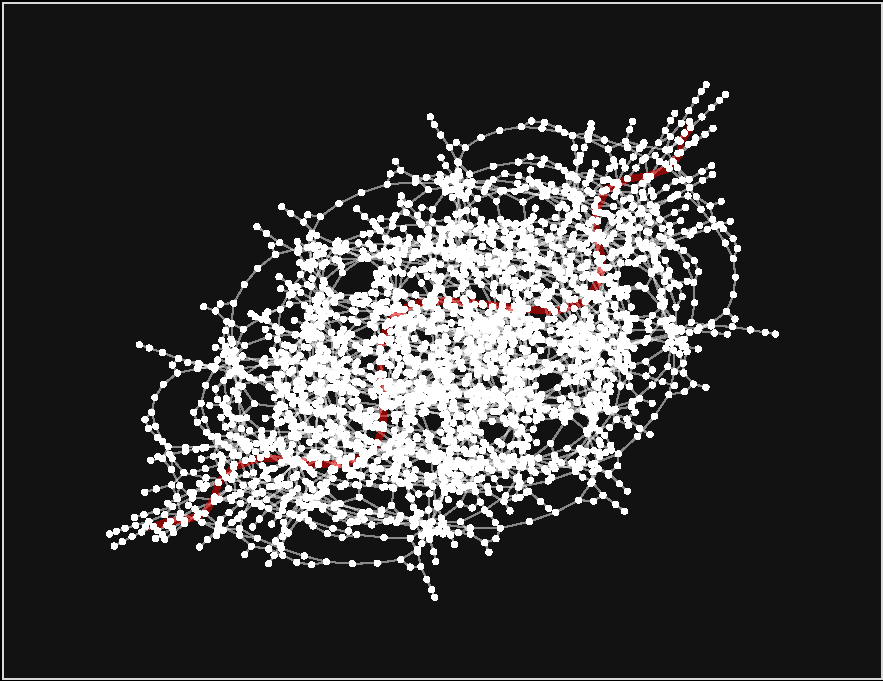
\includegraphics[width=0.8\textwidth]{GrafoNestor.pdf}
\caption{Grafo completo del espacio del problema del juego La Escalera.}
\label{fig:grafo_completo}
\end{figure}

\begin{figure}[H]
\centering
 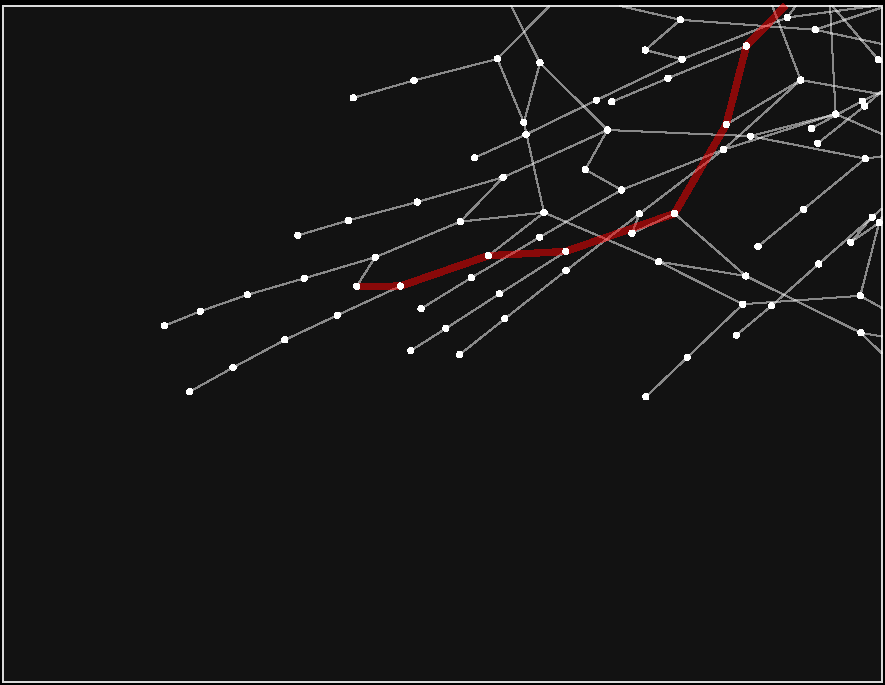
\includegraphics[width=0.8\textwidth]{GrafoNestorZoom.pdf}
\caption{Grafo Zoom.}
\label{fig:grafo_zoom}
\end{figure}

\textbf{El punto de inicio.} Representa la configuración inicial del tablero.

\textbf{El punto de llegada.} Los juegos estructurados tienen un punto de inicio y un punto de llega, es decir la solución del juego. Para el caso del juego la escalera, el punto de llegada se representa por la ubicación de los bloques 

%% inicio aportes 8 de mayo 

\textbf{La ruta óptima.}
El juego La Escalera es un juego estructurado: su tablero puede
encontrarse en un número finito de configuraciones distintas y cada
movimiento válido conduce de una configuración a otra de manera
determinista. El conjunto de todas esas configuraciones posibles,
junto con los movimientos que las conectan, constituye un grafo en el
sentido matemático del término: un conjunto de vértices o nodos (cada
estado del tablero) y un conjunto de aristas (cada movimiento válido que
lleva de un estado a otro), con peso igual a uno en cada arista, ya que
cada movimiento, sin importar si es un avance de una posición o un salto
sobre una ficha del color contrario, tiene el mismo costo unitario dentro
de las reglas del juego \citep{Johnsonbaugh2005}.
 
Dado que el objetivo del juego es pasar de la configuración inicial a la
configuración meta empleando el menor número posible de movimientos, el
problema de encontrar la ruta óptima es, en términos de matemáticas
discretas, el problema de encontrar la trayectoria de longitud mínima
entre dos vértices de un grafo ponderado conexo, para el cual el
algoritmo de Dijkstra ofrece una solución exacta y demostrable.
Formulado por Edsger W.~Dijkstra en 1959, el algoritmo opera asignando a
cada vértice del grafo una etiqueta $L(v)$ que representa la mejor
estimación actual de la longitud del camino más corto desde el vértice de
origen $a$ hasta ese vértice $v$ \citep{Johnsonbaugh2005}. Al iniciar, se
asigna $L(a) = 0$ al vértice de origen (la configuración inicial del
tablero) y $L(v) = \infty$ a todos los demás vértices, representando el
hecho de que aún no se conoce ningún camino hacia ellos. El conjunto $T$
contiene inicialmente la totalidad de los vértices del grafo, que en este
caso son todas las configuraciones posibles del tablero.
 
En cada iteración del algoritmo se selecciona de $T$ el vértice $v$ cuya
etiqueta $L(v)$ es mínima entre todos los que aún no han recibido
etiqueta permanente, se extrae de $T$ (su etiqueta se vuelve permanente)
y se actualizan las etiquetas de todos sus vecinos $x$ que permanecen en
$T$ según la regla:
\begin{equation}
    L(x) = \min \bigl\{L(x),\; L(v) + w(v,x)\bigr\}
\end{equation}
donde $w(v,x)$ es el peso de la arista que une $v$ con $x$, igual a 1 en
el caso del juego La Escalera. El proceso continúa hasta que el vértice
meta $z$ (la configuración completamente intercambiada) abandona $T$ y
adquiere etiqueta permanente, momento en que $L(z)$ contiene la longitud
exacta de la trayectoria más corta desde la configuración inicial hasta
la configuración solución \citep{Johnsonbaugh2005}. Puede demostrarse por
inducción matemática que cuando $v$ es seleccionado en la línea~9 del
algoritmo, $L(v)$ es efectivamente la longitud del camino más corto de
$a$ a $v$, lo que garantiza que el resultado final es el óptimo global y
no una aproximación \citep{Johnsonbaugh2005}.
 
Aplicado al juego La Escalera con $n = 5$ fichas por equipo, el algoritmo
recorre sistemáticamente el grafo del espacio del problema a partir de la
configuración inicial, expandiendo en cada iteración la frontera de
estados alcanzables, hasta que la configuración meta recibe etiqueta
permanente con valor $L(z) = 35$. Este resultado corresponde a la
expresión general $n^2 + 2n$, que para $n = 5$ produce $25 + 10 = 35$
movimientos como longitud de la ruta óptima. La solución óptima sigue el
patrón alternado de movimientos individuales y saltos que puede
describirse como la secuencia
1A-2R-3A-4R-5A-5R-5A-4R-3A-2R-1A (donde A indica una ficha azul y R una
ficha roja, y el número indica cuántas fichas de ese color se mueven
consecutivamente), cuya efectividad queda demostrada precisamente porque
es la trayectoria que el algoritmo de Dijkstra identifica como de costo
mínimo en este grafo.
 
La relevancia de este resultado para el análisis del control inhibitorio
reside en que la ruta óptima encontrada por Dijkstra proporciona una
referencia matemáticamente exacta contra la cual comparar la trayectoria
real de cada aprendiz. Cada movimiento que el estudiante realiza por
fuera de esa ruta óptima constituye una unidad medible de desviación que
puede deberse a exploración deliberada, a error recuperable o a una
decisión impulsiva que cierra caminos de solución. La métrica de
ramificación $C_m = |1 - D_j/D_{\min}|$, donde $D_j$ es la distancia al
nodo meta desde el estado alcanzado tras el movimiento $j$ y $D_{\min}$
es la distancia mínima posible en ese punto, cuantifica precisamente esa
desviación para cada movimiento individual, y toma como referencia la
distancia óptima calculada por el algoritmo de Dijkstra. En este sentido,
el algoritmo no es solo el instrumento computacional que genera la línea
verde de referencia visible en los grafos de trayectorias: es la
demostración matemática de que esa línea representa el camino de menor
costo posible dentro del espacio del problema, lo que otorga validez a su
uso como patrón normativo para el análisis del desempeño y del control
inhibitorio de los aprendices.
 

% Fin de aportes 8 de mayo 
\textbf{Los puntos críticos.} Nodos donde hay múltiples decisiones posibles.

\textbf{Los caminos sin retorno.} Estados sin solución posible.

\textbf{Los bucles.} Retornos a estados anteriores.

\section{Métricas para analizar las trayectorias}

\begin{equation}
C_m = \left|1 - \frac{D_j}{D_{min}}\right|
\end{equation}

\begin{equation}
B_i = \frac{n^2}{2} + 2n
\end{equation}

%
%
%

%Fin de aporte


%
%
%

%Inicio aportes 8 de mayo para revisión 
\section{Fundamento matemático de las métricas de análisis}
\label{sec:fundamento_ecuaciones}
 
El análisis de las trayectorias de resolución del juego La
Escalera requiere traducir el recorrido visual del aprendiz
sobre el grafo en valores cuantitativos que permitan comparar
sesiones, participantes y condiciones de mediación de manera
sistemática. Para ello, la investigación retoma y adapta el
modelo de métricas propuesto por Liévano Chaparro y Molina
Monguí \cite{LievanoMolina2022}, quienes diseñaron dos
indicadores complementarios —\textbf{buclicidad} y
\textbf{ramificación}— a partir del espacio del problema del
juego. A continuación se explica el significado, la estructura
matemática y la pertinencia de cada ecuación en el contexto
de la presente investigación.
 
% -------------------------------------------------------
\subsection*{Movimientos óptimos y espacio del problema}
 
El punto de referencia de todas las métricas es la
\textbf{ruta óptima}: la secuencia mínima de movimientos
válidos que conduce desde el estado inicial hasta el estado
meta sin ningún retroceso ni redundancia. Para el juego La
Escalera con $n$ fichas por color, esta cantidad se obtiene
de la expresión general
 
\begin{equation}
    D_{\min} \;=\; n^{2} + 2n
    \label{eq:optimo}
\end{equation}
 
donde $n$ es el número de fichas por equipo. Con $n = 5$
(versión utilizada en esta investigación), la solución
óptima requiere exactamente $35$ movimientos
\cite{LievanoMolina2022, PaezGonzalez2022}. Este valor
actúa como denominador de referencia en la métrica de
ramificación y como umbral para interpretar la longitud de
los bucles. Cualquier trayectoria real que supere
$D_{\min}$ refleja decisiones no planificadas; la
diferencia entre ambas constituye una medida conductual
del \textbf{control inhibitorio}: a mayor exceso de
movimientos, mayor evidencia de dificultad para suprimir
la respuesta impulsiva y sostener una estrategia deliberada
\cite{Diamond2013}.
 
% -------------------------------------------------------
\subsection*{Métrica de buclicidad}
 
Un \textbf{bucle} ocurre cuando el aprendiz regresa, dentro
de un mismo intento, a una configuración del tablero que
ya había visitado previamente, sin haber llegado al estado
meta entre ambas visitas. Los bucles son informativos porque
reflejan dos fenómenos cognitivos distintos según el nivel
de experiencia del jugador: en un novato, un bucle involuntario
indica que no ha detectado la repetición de estados; en un
jugador más avanzado, un bucle consciente puede ser una
estrategia de exploración o de «no perder» mientras reorganiza
la planificación \cite{LievanoMolina2022}.
 
La longitud mínima de un bucle completo —el número de
movimientos necesarios para salir y regresar a un nodo—
depende de la cantidad de fichas involucradas. Liévano
Chaparro y Molina Monguí distinguen dos casos.
 
\medskip
\noindent\textbf{Caso con cantidad par de fichas involucradas:}
\begin{equation}
    B_{i} \;=\; \frac{n^{2}}{2} + 2n
    \label{eq:bucle_par}
\end{equation}
 
\noindent\textbf{Caso con cantidad impar de fichas involucradas:}
\begin{equation}
    B_{i} \;=\; \frac{n^{2}}{2} + 2n - \frac{1}{2}
    \label{eq:bucle_impar}
\end{equation}
 
Ambas expresiones se unifican en la forma general
\begin{equation}
    B_{i} \;=\; \frac{n^{2}}{2} + 2n + C
    \label{eq:bucle_general}
\end{equation}
 
donde $C$ es una constante que toma el valor $0$ en el caso
par y $-\tfrac{1}{2}$ en el caso impar, y $n$ es el número
de fichas involucradas en el bucle. Las ecuaciones contemplan
únicamente bucles completos que siguen la ruta óptima,
desviándose de ella y retornando; en la práctica se acepta
una tolerancia de aproximadamente $\pm 2$ movimientos cuando
la configuración del tablero impide transitar exactamente
por el camino previsto \cite{LievanoMolina2022}.
 
A partir de la buclicidad por intento se define la
\textbf{buclicidad por experiencia}
 
\begin{equation}
    B_{e} \;=\; \frac{1}{m}\sum_{j=1}^{m} B_{i,j}
    \label{eq:bucle_exp}
\end{equation}
 
donde $m$ es el número total de intentos registrados. Este
promedio permite observar si el tamaño o la frecuencia de
los bucles disminuye a medida que el aprendiz acumula
experiencia, lo que constituye evidencia de aprendizaje
progresivo.
 
En el contexto de la presente investigación con estudiantes
con TEA nivel~1, la buclicidad adquiere una relevancia
adicional: los retornos involuntarios y frecuentes a estados
ya visitados son coherentes con las dificultades en el
control inhibitorio sostenido y en la memoria de trabajo
que caracterizan a esta población \cite{Geurts2009,
Diamond2013}. La comparación de los valores de $B_{e}$
entre la sesión sin mediación y la sesión con activación
de los cubos inteligentes permitirá explorar si la
herramienta con agentividad reduce la tasa de bucles
involuntarios.
 
\begin{figure}[H]
\centering
\fbox{\parbox{0.82\textwidth}{%
    \textcolor{red}{\textbf{[INSERTAR AQUÍ]} Gráfica de buclicidad
    por intento ($B_i$) para ambos participantes. Eje $x$: número
    de intento; eje $y$: valor $B_i$. Comparar sesión sin mediación
    (línea/color A) vs. sesión con cubos (línea/color B).}
}}
\caption{Buclicidad por intento: comparación entre sesiones.}
\label{fig:grafica_buclicidad}
\end{figure}
 
% -------------------------------------------------------
\subsection*{Métrica de ramificación}
 
La \textbf{ramificación} mide la calidad de cada movimiento
individual en relación con la ruta óptima. Formalmente, la
\textbf{calidad del movimiento} $C_m$ se define como
 
\begin{equation}
    C_{m} \;=\; \left|1 - \frac{D_{j}}{D_{\min}}\right|
    \label{eq:calidad_movimiento}
\end{equation}
 
donde $D_{j}$ es la distancia —en número de movimientos
válidos restantes— desde el estado actual del jugador hasta
el estado meta, y $D_{\min}$ es la distancia mínima posible
desde ese mismo estado hasta la meta (es decir, la longitud
del camino óptimo restante desde ese nodo). Cuando el
aprendiz elige el movimiento óptimo disponible, $D_{j} =
D_{\min}$ y $C_m = 0$; a medida que el movimiento elegido
lo aleja de la meta, el cociente $D_{j}/D_{\min}$ aumenta
y $C_m$ crece. Un valor de $C_m$ cercano a cero en todos
los movimientos de un intento indica que el aprendiz siguió
la ruta óptima; valores dispersos y elevados reflejan
exploración no planificada o decisiones impulsivas
\cite{LievanoMolina2022}.
 
La \textbf{ramificación por intento} agrega los valores
individuales de calidad a lo largo de los $n_i$ movimientos
de un intento:
 
\begin{equation}
    R_{i} \;=\; \sum_{k=1}^{n_i} C_{m,k}
    \label{eq:ramif_intento}
\end{equation}
 
Y la \textbf{ramificación por experiencia} promedia sobre
los $n$ intentos realizados:
 
\begin{equation}
    R_{e} \;=\; \frac{1}{n}\sum_{j=1}^{n} R_{i,j}
    \label{eq:ramif_exp}
\end{equation}
 
En los grafos de dispersión (eje $x$: número de movimiento
dentro del intento; eje $y$: valor de $C_m$), los puntos
cercanos al eje horizontal representan movimientos óptimos
y los puntos dispersos hacia arriba representan desviaciones
de la ruta óptima. La evolución de esta dispersión a lo
largo de los intentos —desde alta variabilidad inicial
hacia concentración en el eje— refleja la consolidación
del esquema de solución \cite{LievanoMolina2022}.
 
En la presente investigación, la ramificación se interpreta
en clave de control inhibitorio: cada movimiento con
$C_m > 0$ puede leerse como un episodio en el que el
aprendiz no inhibió la respuesta disponible más inmediata
en favor de la más eficiente. Los patrones de ramificación
diferenciales entre la sesión sin cubos y la sesión con
cubos inteligentes, correlacionados con los mapas de
potencia alfa relativa (Alpha TRP) obtenidos con EEG,
constituyen la evidencia integrada central del análisis
de resultados de esta tesis.
 
\begin{figure}[H]
\centering
\fbox{\parbox{0.82\textwidth}{%
    \textcolor{red}{\textbf{[INSERTAR AQUÍ]} Gráfica de ramificación
    por intento para ambos participantes. Dispersión de $C_m$
    (eje $y$) vs. número de movimiento en el intento (eje $x$).
    Sesión sin mediación vs. sesión con cubos. Incluir línea
    de tendencia o curva suavizada si es posible.}
}}
\caption{Ramificación por movimiento: comparación entre sesiones.}
\label{fig:grafica_ramificacion}
\end{figure}
 
\medskip
\noindent La Tabla~\ref{tab:resumen_metricas} presenta un
resumen de las ecuaciones, su dominio de aplicación y su
interpretación en el marco de esta investigación.
 
\begin{table}[H]
\centering
\caption{Resumen de métricas para el análisis de trayectorias}
\label{tab:resumen_metricas}
\renewcommand{\arraystretch}{1.35}
\resizebox{\textwidth}{!}{%
\begin{tabular}{|p{3.2cm}|p{3.5cm}|p{3.5cm}|p{4.2cm}|}
\hline
\textbf{Métrica} & \textbf{Ecuación} & \textbf{Interpretación cognitiva} & \textbf{Relevancia en TEA nivel~1} \\
\hline
Ruta óptima & $D_{\min} = n^2 + 2n$ &
Referencia de la planificación perfecta &
Permite medir la brecha entre la conducta real y la conducta estratégica \\
\hline
Buclicidad por intento & $B_i = \tfrac{n^2}{2} + 2n + C$ &
Retorno a estados ya visitados; refleja ausencia de memoria de trabajo activa &
Indicador de dificultad inhibitoria sostenida: bucles frecuentes = menor control ejecutivo \\
\hline
Buclicidad por experiencia & $B_e = \tfrac{1}{m}\sum B_{i,j}$ &
Evolución del aprendizaje: $B_e$ decreciente indica menor impulsividad acumulada &
Permite comparar progreso intra-sesión entre condición sin y con mediación \\
\hline
Calidad del movimiento & $C_m = |1 - D_j/D_{\min}|$ &
Distancia relativa al óptimo en cada decisión puntual &
$C_m = 0$: decisión planificada; $C_m > 0$: respuesta impulsiva no inhibida \\
\hline
Ramificación por intento & $R_i = \sum C_{m,k}$ &
Exploración acumulada respecto a la ruta óptima en un intento &
Valor alto: mayor dificultad para sostener la estrategia \\
\hline
Ramificación por experiencia & $R_e = \tfrac{1}{n}\sum R_{i,j}$ &
Tendencia general de la toma de decisiones a lo largo de la sesión &
Comparación entre sesiones: efecto de los cubos sobre la planificación global \\
\hline
\end{tabular}}
\end{table}
 
 

% 2 -> Fin cap agregado para revisión

% FINN




\chapter{Metodología}

\section{Diseño de la investigación}

\begin{figure}[h]
    \centering
    % Ajusta los valores de trim (en mm o cm) hasta que la imagen se vea bien
    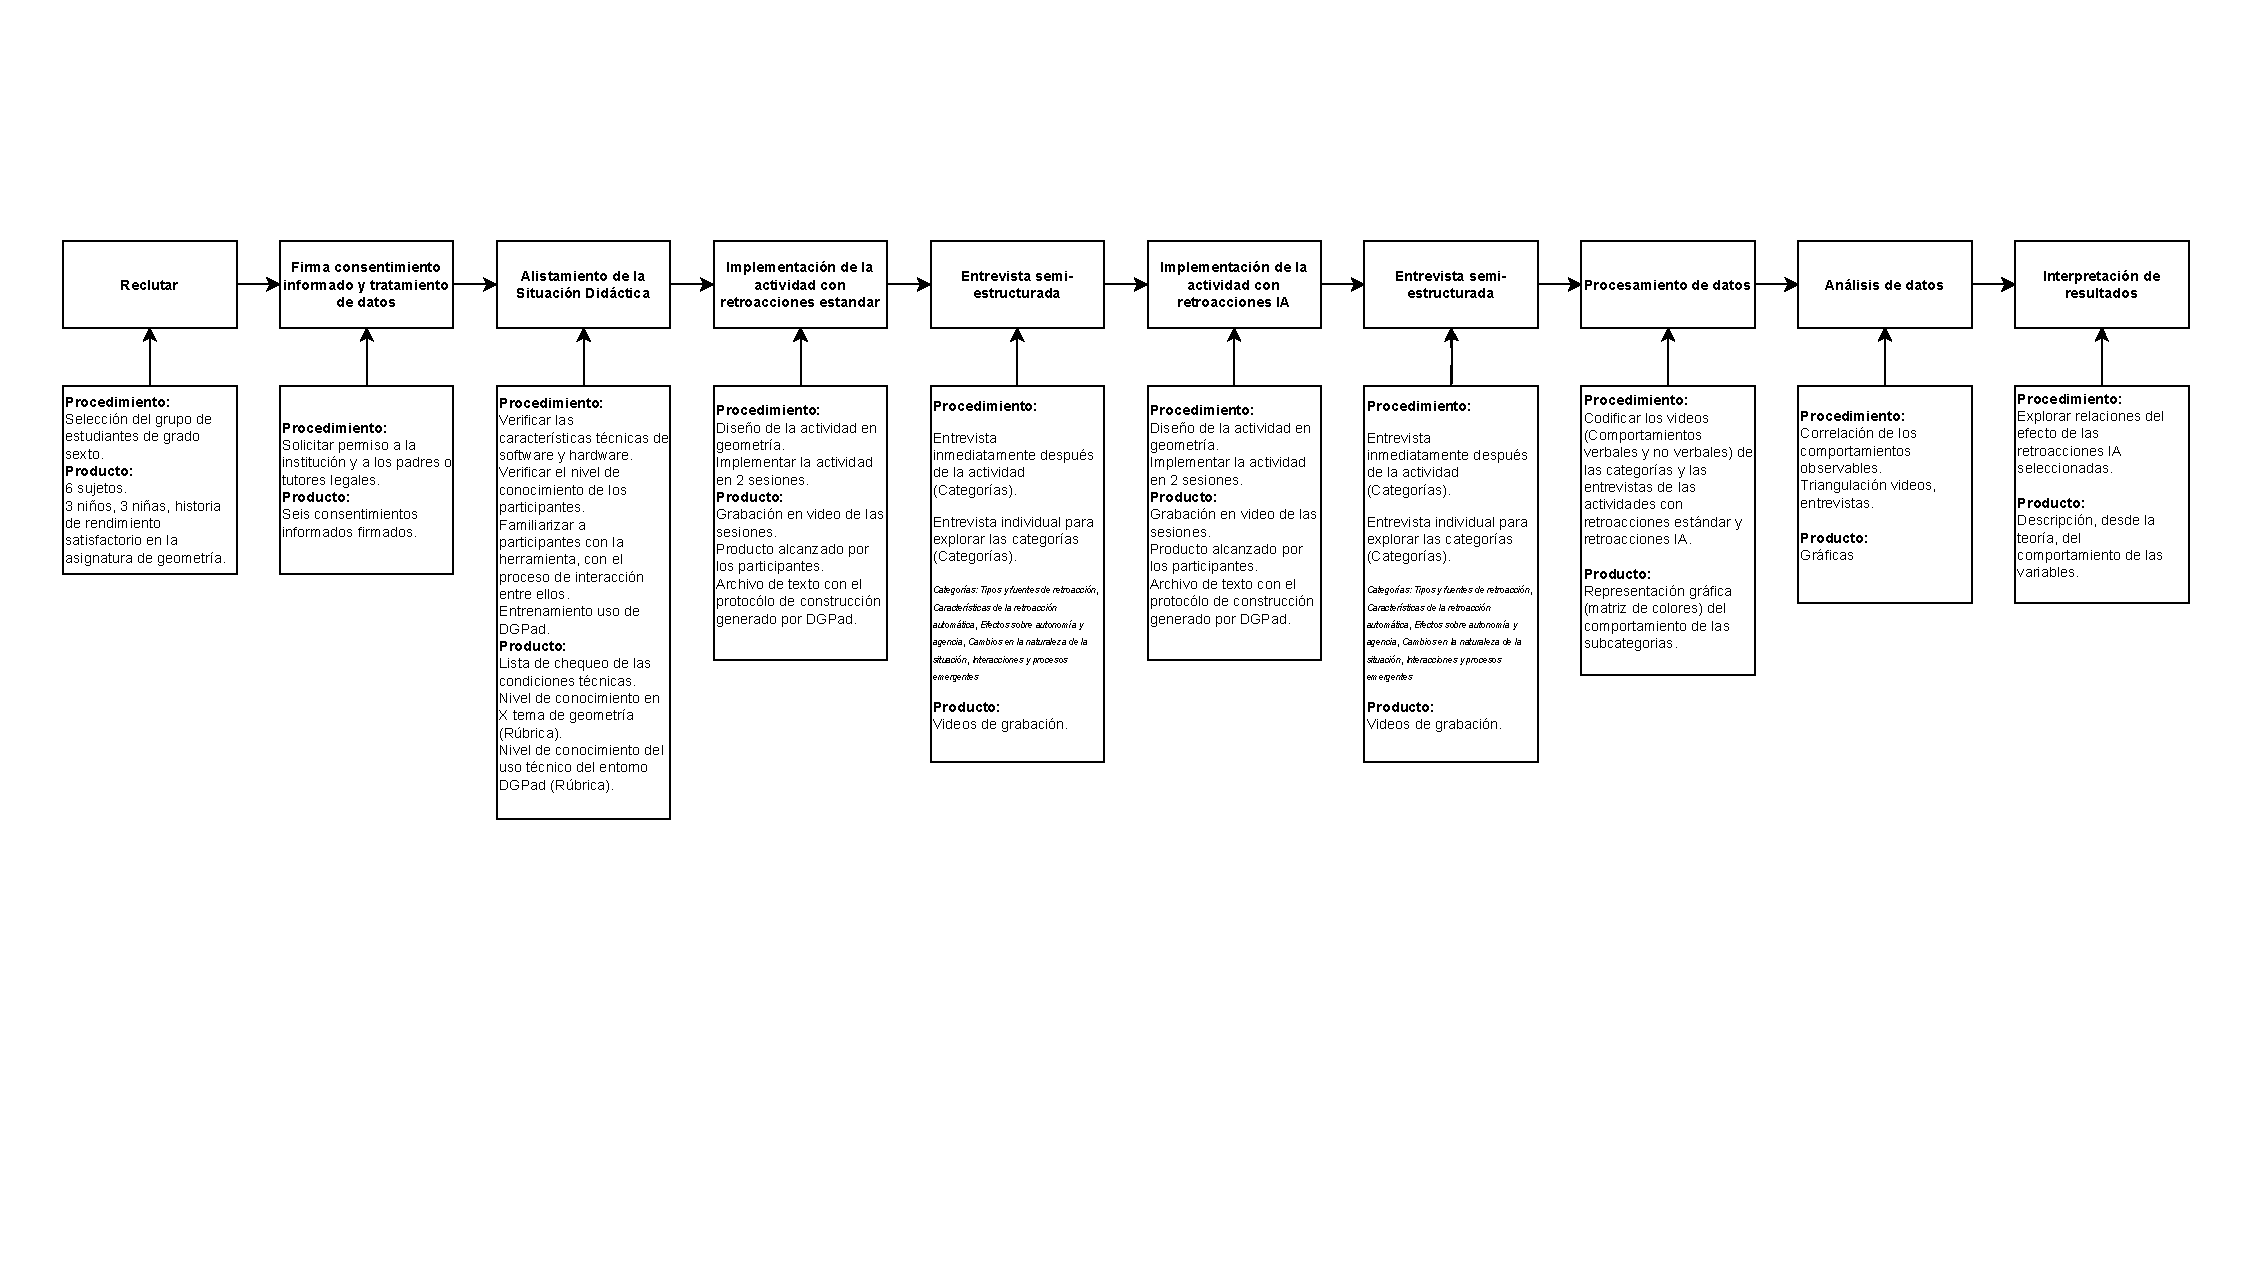
\includegraphics[width=\linewidth, trim={0.2cm 0.5cm 0.5cm 0.5cm}, clip]{Metodología.pdf}
    \caption{Diseño metodológico}
    \label{fig:placeholder}
\end{figure}



\section{Propuesta estructural integradora}

Se propone un sistema multiagente fundamentado en:

\begin{itemize}
    \item Dimensiones del control inhibitorio.
    \item Modelo de memoria de trabajo.
    \item Modelo circumplex de regulación emocional.
    \item Enfoque de resolución de problemas matemáticos.
\end{itemize}

El sistema está compuesto por tres agentes funcionales: \textit{Pausar}, \textit{Pensar} y \textit{Actuar}. Cada agente interviene sobre dimensiones conductuales, cognitivas y emocionales.


\subsection{Guión experimental TEA Nivel 1}

\subsubsection{Capa Teórica}

\begin{figure}[ht]
\centering
\resizebox{0.8\textwidth}{!}{%
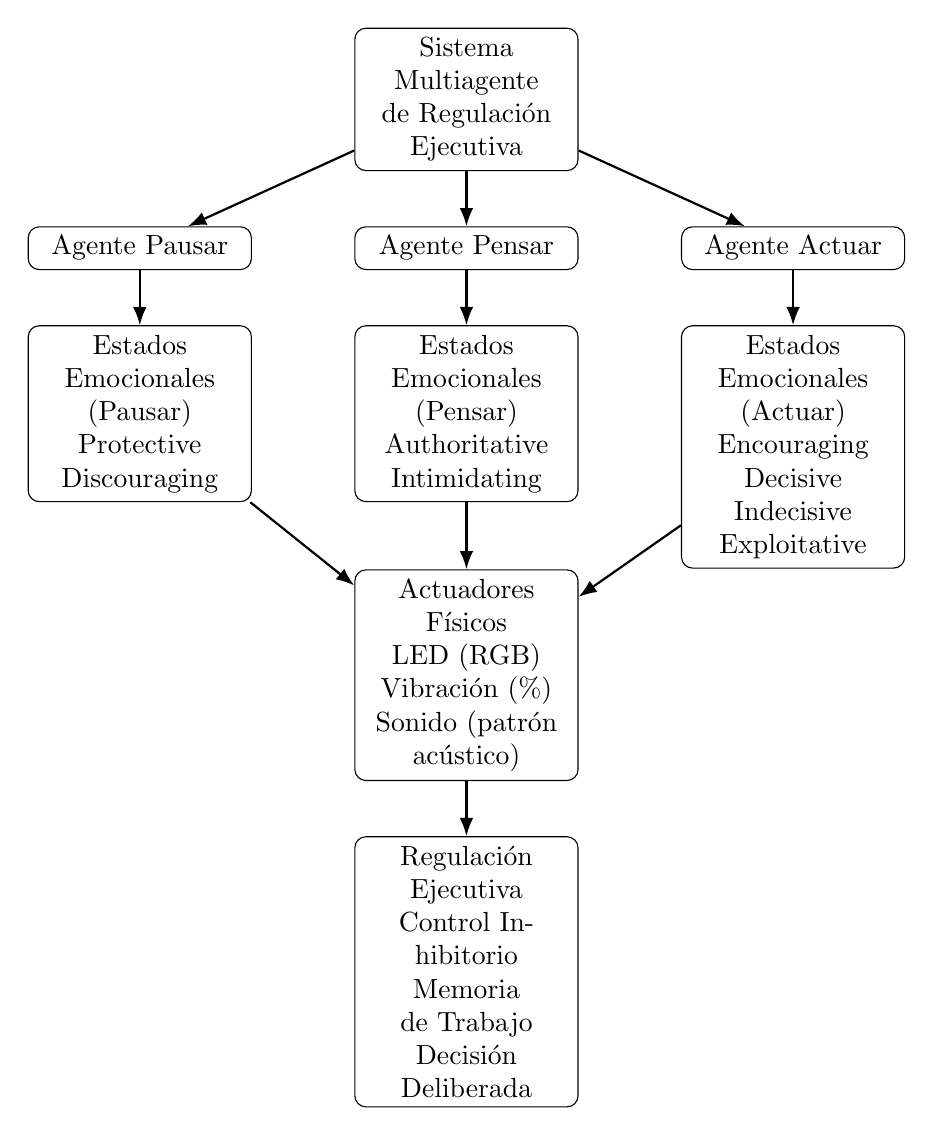
\begin{tikzpicture}[
node distance=0.7cm and 1.3cm,
box/.style={rectangle, draw, rounded corners, align=center, text width=2.6cm},
arrow/.style={-{Latex}, thick}
]

% Nivel 1
\node[box] (system) {Sistema Multiagente \\ de Regulación Ejecutiva};

% Nivel 2 - Agentes
\node[box, below left=of system] (pausar) {Agente Pausar};
\node[box, below=of system] (pensar) {Agente Pensar};
\node[box, below right=of system] (actuar) {Agente Actuar};

% Nivel 3 - Estados emocionales por agente

\node[box, below=of pausar] (emo_pausar) {
Estados Emocionales \\ (Pausar) \\
Protective \\ Discouraging
};

\node[box, below=of pensar] (emo_pensar) {
Estados Emocionales \\ (Pensar) \\
Authoritative \\ Intimidating
};

\node[box, below=of actuar] (emo_actuar) {
Estados Emocionales \\ (Actuar) \\
Encouraging \\ Decisive \\ Indecisive \\ Exploitative
};

% Nivel 4 - Actuadores
\node[box, below=3.8cm of pensar] (actuadores) {
Actuadores Físicos \\
LED (RGB) \\
Vibración (\%) \\
Sonido (patrón acústico)
};

% Nivel 5 - Resultado
\node[box, below=of actuadores] (resultado) {
Regulación Ejecutiva \\
Control Inhibitorio \\
Memoria de Trabajo \\
Decisión Deliberada
};

% Flechas
\draw[arrow] (system) -- (pausar);
\draw[arrow] (system) -- (pensar);
\draw[arrow] (system) -- (actuar);

\draw[arrow] (pausar) -- (emo_pausar);
\draw[arrow] (pensar) -- (emo_pensar);
\draw[arrow] (actuar) -- (emo_actuar);

\draw[arrow] (emo_pausar) -- (actuadores);
\draw[arrow] (emo_pensar) -- (actuadores);
\draw[arrow] (emo_actuar) -- (actuadores);

\draw[arrow] (actuadores) -- (resultado);

\end{tikzpicture}
}
\caption{Modelo multinivel jerárquico con estados emocionales específicos por agente}
\end{figure}







\subsubsection{Capa Técnica}

\begin{table}[ht]
\centering
\small
\caption{Configuración de cubos según emoción y agente}

\resizebox{\textwidth}{!}{
\begin{tabular}{|l|l|c|c|c|l|}
\hline
\textbf{Emoción} & \textbf{Agente} & \textbf{LED (RGB)} & \textbf{Vibración} & \textbf{Sonido} & \textbf{Función Ejecutiva} \\
\hline
Protective & Pausar & Azúl suave & 20\% & Grave continuo & Regulación emocional \\
Discouraging & Pausar & Azul intermitente & 10\% & Descendente & Inhibición leve \\
Authoritative & Pausar/Actuar & Azul intenso & 35\% & Pulso firme & Control estructural \\
Indecisive & Pensar & Amarillo tenue & 30\% & Bajo repetitivo & Exploración estratégica \\
Exploitative & Pensar & Naranja & 45\% & Medio sostenido & Evaluación de opciones \\
Encouraging & Pensar/Actuar & Verde-turquesa & 70\% & Arpegio & Refuerzo positivo \\
Decisive & Actuar & Verde brillante & 80\% & Ascendente & Confirmación deliberada \\
Intimidating & Pausar & Rojo tenue & 50\% & Grave abrupto & Alerta inhibitoria \\
\hline
\end{tabular}
}
\end{table}






\begin{table}[ht]
\centering
\caption{Tabla complementaria de codificación cromática del sistema}
\renewcommand{\arraystretch}{1.2}
\begin{tabular}{|p{3cm}|p{3cm}|p{3cm}|p{4cm}|}
\hline
\textbf{Color (Nombre)} & \textbf{Código RGB} & \textbf{Categoría Cromática} & \textbf{Función Reguladora en el Sistema} \\
\hline

Azul suave 
& (0, 0, 150) 
& Frío – Baja activación 
& Induce calma y favorece regulación emocional inicial \\

\hline

Azul intermitente 
& (0, 0, 200) 
& Frío – Activación moderada 
& Señal de advertencia leve para inhibición conductual \\

\hline

Azul intenso 
& (0, 0, 255) 
& Frío – Alta directividad 
& Refuerza control estructural y autoridad reguladora \\

\hline

Amarillo tenue 
& (255, 255, 102) 
& Cálido – Activación cognitiva 
& Estimula exploración y análisis reflexivo \\

\hline

Naranja medio 
& (255, 140, 0) 
& Cálido – Activación estratégica 
& Promueve evaluación de alternativas \\

\hline

Verde turquesa 
& (64, 224, 208) 
& Neutro-regulador 
& Refuerzo positivo y estabilidad emocional \\

\hline

Verde brillante 
& (0, 255, 0) 
& Neutro – Confirmación 
& Indica validación y consolidación de decisión \\

\hline

Rojo tenue 
& (200, 0, 0) 
& Cálido – Alta activación 
& Señal de alerta inhibitoria ante impulsividad \\

\hline

\end{tabular}
\end{table}



El flujo operativo del sistema sigue la secuencia:

\begin{enumerate}
    \item Detección, por parte del docente, de un intento impulsivo, y activación del agente Pausar.
    \item Estabilización cognitiva y activación del agente Pensar.
    \item Confirmación deliberada por parte del docente y activación del agente Actuar.
\end{enumerate}


\section{Participantes}

%%inicio aportes 8 de mayo 

\section{Materiales}
Para la investigación se emplea un prototipo de cubos inteligentes.
Además, se emplea una interface para el control de los cubos inteligentes que emplea la técnica de ``Mago de Oz''.
%%%%%% ******* %%%%%%% Foto de todo el prototipo
\begin{figure}[h]
    \centering
    % Ajusta los valores de trim (en mm o cm) hasta que la imagen se vea bien
    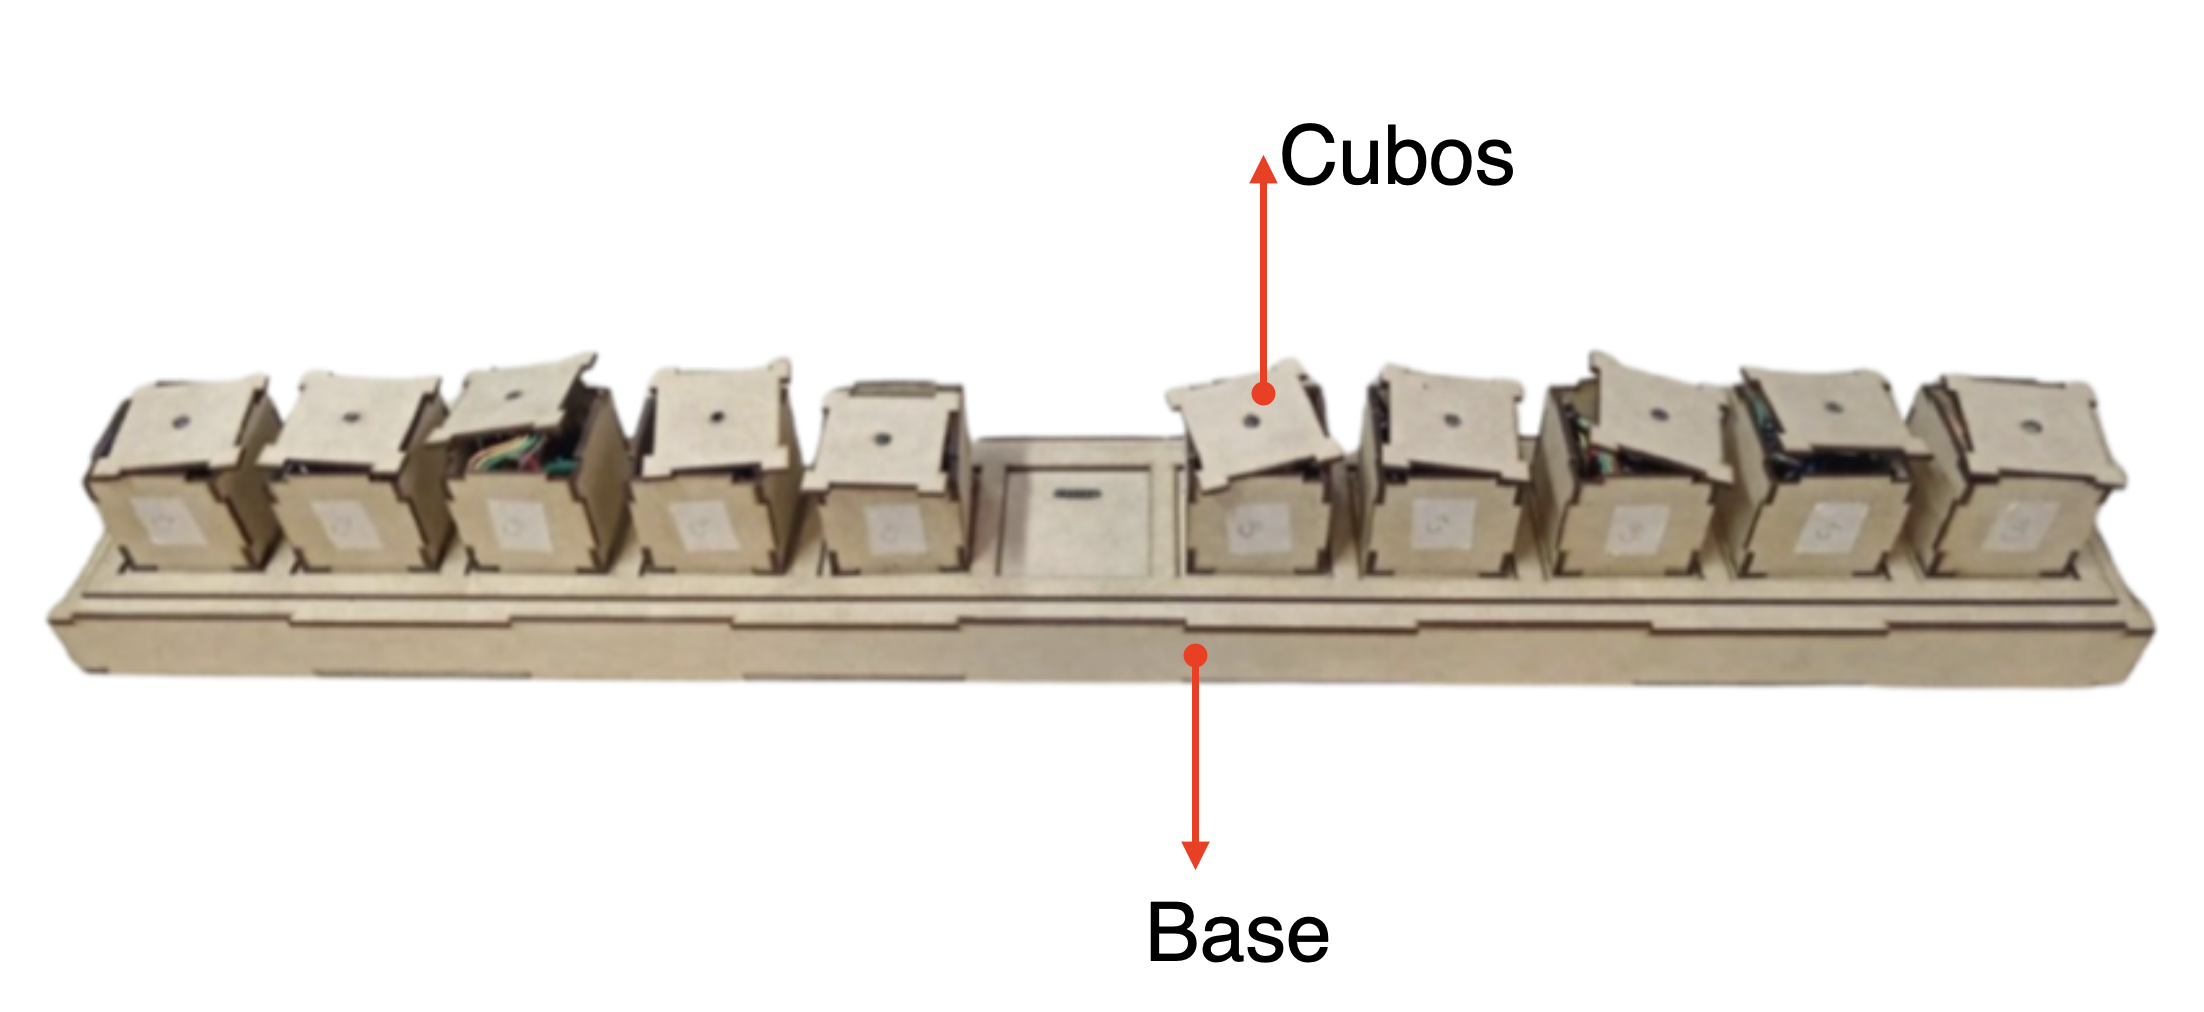
\includegraphics[width=\linewidth, trim={0.2cm 0.5cm 0.5cm 0.5cm}, clip]{Juego Inteligente.png}
    \caption{Prototipo ensamblado del tablero de cubos inteligentes: los diez cubos dispuestos en dos grupos de cinco sobre la base de madera, con la posición central vacía correspondiente al espacio intercambiable del juego La Escalera.}
    \label{fig:placeholder}
\end{figure}

 
\subsection{Descripción técnica de los cubos inteligentes}
El diseño mecánico, electrónico y lógico de los cubos fue desarrollado por el módulo INNOVA del Centro ACACIA de la Universidad..... xxx.
%%%%%% ******* %%%%%%% Foto Cubo Frente, Isométrica, Destapado, Encendido.
\begin{figure}[h]
    \centering
    % Ajusta los valores de trim (en mm o cm) hasta que la imagen se vea bien
    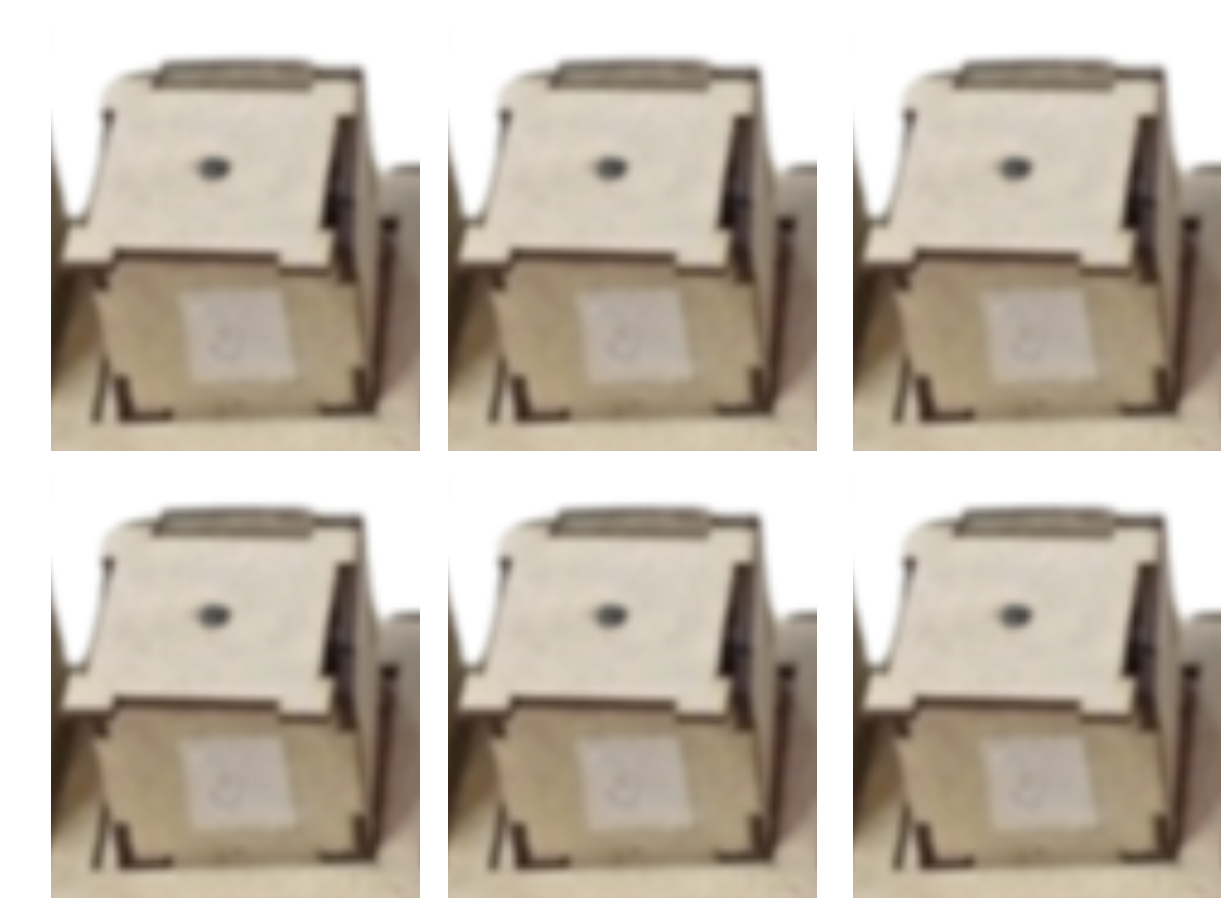
\includegraphics[width=\linewidth, trim={0.2cm 0.5cm 0.5cm 0.5cm}, clip]{vistascubo.png}
    \caption{Vista frontal de un cubo inteligente individual, con la tapa superior entreabierta y la etiqueta identificadora visible en la cara frontal.}
    \label{fig:placeholder}
\end{figure}
%%% Explicar las vistas de la figura anterior.
%%%%%% ******* %%%%%%% Diagrama Electrónico
El núcleo de procesamiento de cada cubo es un microcontrolador
ESP32-C3 SuperMini, que se conecta por WiFi como estación a la red
inalámbrica generada por el \textit{Master} para recibir sus
instrucciones. Los periféricos de salida conectados al microcontrolador
son tres: un diodo LED de tipo RGB capaz de producir cualquier
combinación de color mediante la modulación independiente de sus tres
canales (rojo, verde y azul, con valores entre 0 y 255 en cada canal),
un motor de vibración de tipo moneda con regulación de intensidad por
modulación de ancho de pulso (PWM), y un altavoz piezoeléctrico o
buzzer con capacidad de emitir tonos de frecuencia y duración
controladas programáticamente. El sistema integra así una respuesta
multimodal completa —luz, vibración y sonido—; la integración del
componente sonoro en el mensaje de comando enviado por el
\textit{Master} se completará en una fase posterior de desarrollo del
firmware. La alimentación del cubo se realiza mediante batería
recargable Li-Po de 3.7~V y 180~mAh,

%%%%%% ******* %%%%%%% Expicar Código + Diagrama de código "Algorithm"

\subsection{Funcionamiento electrónico de los cubos}

El cubo inteligente integra, en un volumen reducido de madera, la
electrónica de control, los actuadores multisensoriales y el sistema
de acoplamiento con la base del tablero. La Figura~\ref{fig:cubo-arquitectura}
organiza estos componentes en un esquema de bloques.

El núcleo de procesamiento de cada cubo es un microcontrolador
ESP32-C3 SuperMini, alimentado por una batería recargable Li-Po de
3.7~V y 180~mAh. El ESP32-C3 recibe por WiFi las instrucciones
enviadas por el ESP32 maestro y las traduce en señales de control
hacia el LED RGB y el motor de vibración, cuyos parámetros de
operación —color e intensidad, respectivamente— llegan directamente en
el mensaje transmitido por el maestro. El cubo incorpora además un
buzzer como tercer actuador multisensorial previsto en el diseño del
sistema, cuya integración en el mensaje de comando del maestro se
completará en una fase posterior de desarrollo del firmware. Cada cubo
se fija a su posición en el tablero mediante una interfaz de
acoplamiento magnético con la casilla correspondiente de la base, que
además cierra un contacto empleado por la base para detectar la
presencia del cubo en esa posición.

\begin{figure}[H]
\centering
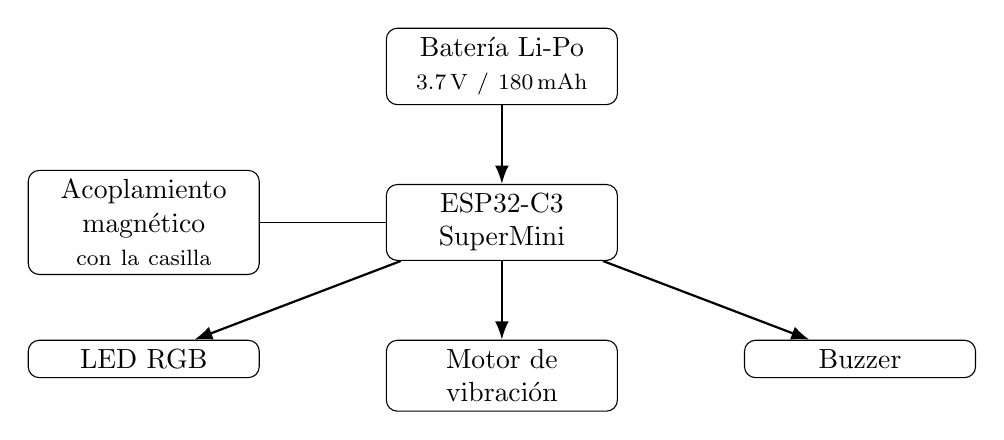
\begin{tikzpicture}[
node distance=1.0cm and 1.6cm,
box/.style={rectangle, draw, rounded corners, align=center, text width=2.7cm},
arrow/.style={-{Latex}, thick},
mech/.style={thin}
]

\node[box] (cubo_esp32) {ESP32-C3 \\ SuperMini};
\node[box, above=of cubo_esp32] (cubo_alim) {Batería Li-Po \\ \footnotesize 3.7\,V / 180\,mAh};
\node[box, left=of cubo_esp32] (cubo_acople) {Acoplamiento \\ magnético \\ \footnotesize con la casilla};
\node[box, below left=of cubo_esp32] (cubo_led) {LED RGB};
\node[box, below=of cubo_esp32] (cubo_vib) {Motor de \\ vibración};
\node[box, below right=of cubo_esp32] (cubo_buz) {Buzzer};

\draw[arrow] (cubo_alim) -- (cubo_esp32);
\draw[mech] (cubo_acople) -- (cubo_esp32);
\draw[arrow] (cubo_esp32) -- (cubo_led);
\draw[arrow] (cubo_esp32) -- (cubo_vib);
\draw[arrow] (cubo_esp32) -- (cubo_buz);

\end{tikzpicture}
\caption{Arquitectura interna del cubo inteligente: un microcontrolador
ESP32-C3 SuperMini gestiona los tres actuadores multisensoriales (LED
RGB, motor de vibración y buzzer) y se alimenta de una batería Li-Po.
El trazo delgado hacia el acoplamiento magnético señala una relación
mecánica de posicionamiento con la casilla de la base, distinta de las
señales de control eléctricas que el microcontrolador gestiona
directamente sobre los tres actuadores.}
\label{fig:cubo-arquitectura}
\end{figure}

El comportamiento observable del cubo —su color, su patrón de
vibración y, cuando se complete la integración del firmware, su
sonido— depende de la instrucción que recibe desde el ESP32 maestro.
La forma en que esa instrucción se genera, se transmite y llega hasta
el cubo es objeto de la siguiente subsección.

\subsection{Funcionamiento lógico de los cubos}

Mientras que la subsección anterior describió los componentes físicos
del cubo, esta subsección explica cómo se genera, transmite y ejecuta
una instrucción dentro del sistema completo que permite al docente
controlarlo.

\begin{figure}[H]
\centering
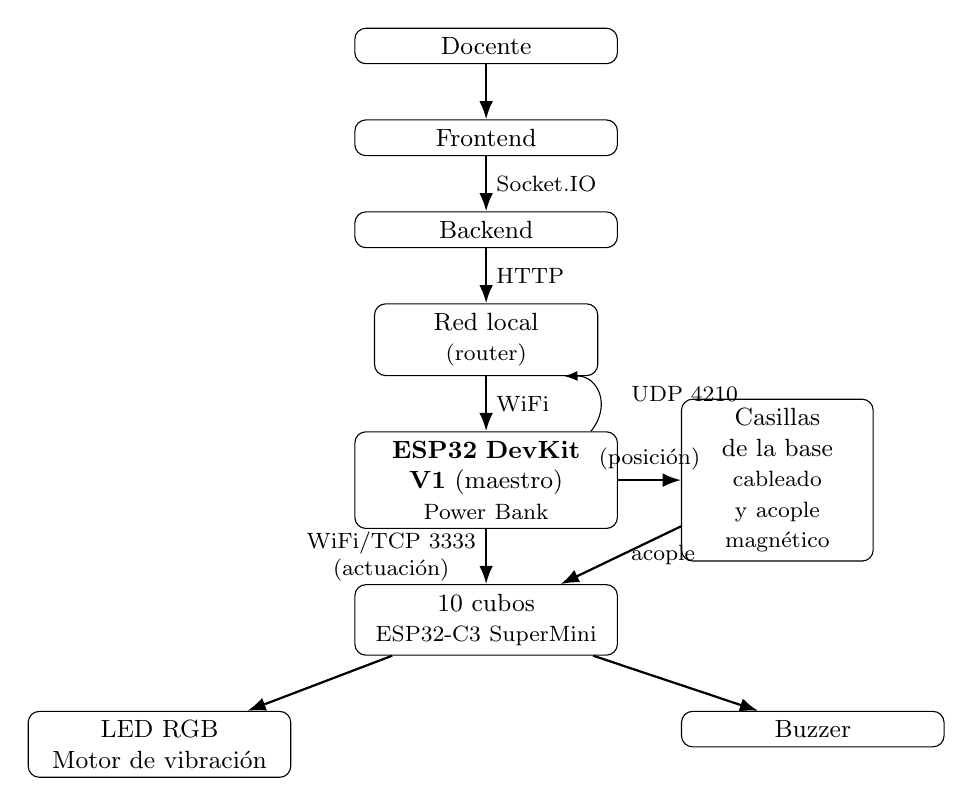
\begin{tikzpicture}[
node distance=0.7cm and 0.8cm,
box/.style={rectangle, draw, rounded corners, align=center, text width=3.1cm, font=\small},
arrow/.style={-{Latex}, thick},
arrowaux/.style={-{Latex}, thin},
arrownv/.style={-{Latex}, thick, dashed}
]

\node[box] (arch_docente) {Docente};
\node[box, below=of arch_docente] (arch_frontend) {Frontend};
\node[box, below=of arch_frontend] (arch_backend) {Backend};
\node[box, below=of arch_backend, text width=2.6cm] (arch_router) {Red local \\ \footnotesize (router)};
\node[box, below=of arch_router] (arch_maestro) {\textbf{ESP32 DevKit V1} (maestro) \\ \footnotesize Power Bank};
\node[box, below=of arch_maestro] (arch_cubos) {10 cubos \\ \footnotesize ESP32-C3 SuperMini};
\node[box, right=of arch_maestro, text width=2.2cm] (arch_casillas) {Casillas de la base \\ \footnotesize cableado y acople magnético};
\node[box, below left=of arch_cubos] (arch_ledvib) {LED RGB \\ Motor de vibración};
\node[box, below right=of arch_cubos] (arch_buzzer) {Buzzer};

\draw[arrow] (arch_docente) -- (arch_frontend);
\draw[arrow] (arch_frontend) -- node[right, font=\footnotesize] {Socket.IO} (arch_backend);
\draw[arrow] (arch_backend) -- node[right, font=\footnotesize] {HTTP} (arch_router);
\draw[arrow] (arch_router) -- node[right, font=\footnotesize] {WiFi} (arch_maestro);
\draw[arrowaux] (arch_maestro) to[bend right=65, looseness=1.4] node[right, font=\footnotesize, xshift=0.3cm] {UDP 4210} (arch_router);
\draw[arrow] (arch_maestro) -- node[left, font=\footnotesize, align=center] {WiFi/TCP 3333\\(actuación)} (arch_cubos);
\draw[arrow] (arch_maestro) -- node[above, font=\footnotesize, sloped] {(posición)} (arch_casillas);
\draw[arrow] (arch_casillas) -- node[right, font=\footnotesize] {acople} (arch_cubos);
\draw[arrow] (arch_cubos) -- (arch_ledvib);
\draw[arrow] (arch_cubos) -- (arch_buzzer);

\end{tikzpicture}
\caption{Arquitectura general del sistema. El ESP32 DevKit V1 (maestro)
se conecta a la red local del laboratorio a través de un router y
sostiene, hacia los diez cubos, dos canales independientes: uno de
actuación (WiFi, mediante una conexión TCP en el puerto 3333), por el
que transmite los comandos de color y vibración —el sonido se
incorporará a este mismo canal en una fase posterior de desarrollo—, y
uno de posición (cableado de las casillas de la base y su acoplamiento
magnético con cada cubo), por el que detecta en qué posición del
tablero se encuentra cada uno.}
\label{fig:arquitectura-general}
\end{figure}

La Figura~\ref{fig:arquitectura-general} representa esa cadena. El
docente interactúa directamente con el frontend, una interfaz web que
traduce cada acción —Pausar, Pensar o Actuar— seleccionada sobre un
cubo en un mensaje enviado al backend mediante Socket.IO. El backend
conserva ese mensaje y lo entrega, sin modificarlo, al ESP32 maestro
cuando este lo solicita mediante peticiones HTTP periódicas a través
del router de la red del laboratorio. El maestro transmite la
instrucción al cubo correspondiente mediante una conexión TCP en el
puerto 3333 sobre el canal WiFi de actuación, y este activa sus
actuadores en consecuencia. De manera independiente, la base emplea el
cableado de cada casilla y el acoplamiento magnético con el cubo
asentado en ella para determinar qué posición del tablero está
ocupada en cada momento; este canal de posición se describe con mayor
detalle en la subsección «Funcionamiento electrónico de la base de los
cubos».

\begin{figure}[H]
\centering
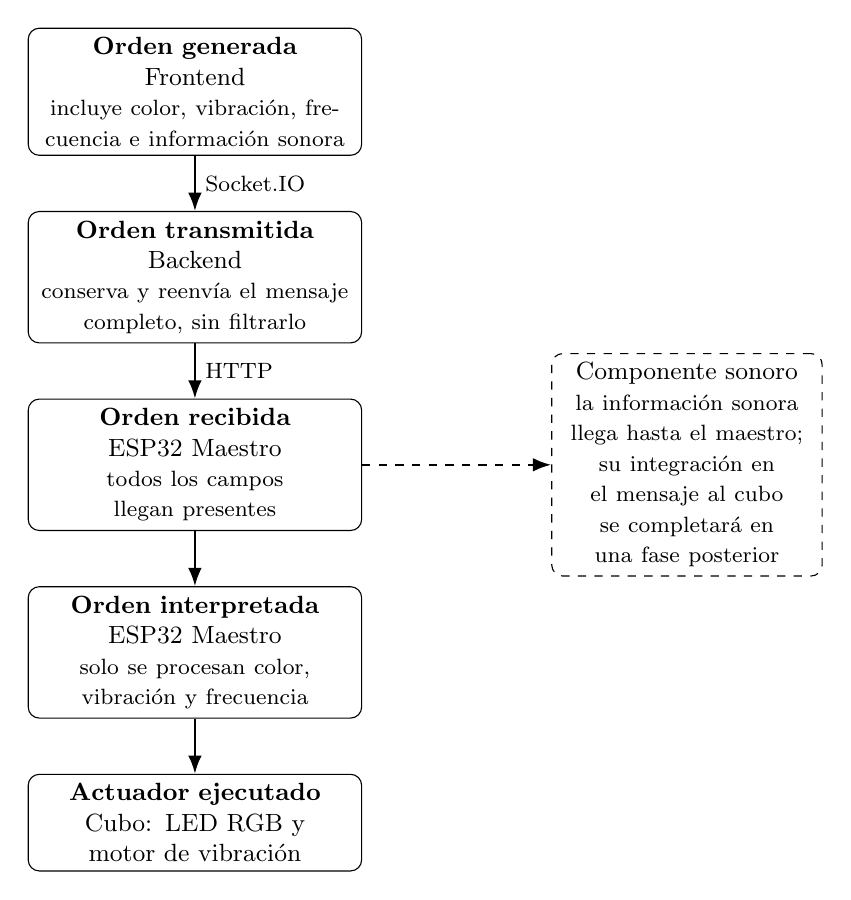
\begin{tikzpicture}[
node distance=0.7cm and 2.4cm,
box/.style={rectangle, draw, rounded corners, align=center, text width=4.0cm, font=\small},
sidebox/.style={rectangle, draw, rounded corners, align=center, text width=3.2cm, font=\small},
arrow/.style={-{Latex}, thick},
arrownv/.style={-{Latex}, thick, dashed}
]

\node[box] (flow_gen) {\textbf{Orden generada} \\ Frontend \\ \footnotesize incluye color, vibración, frecuencia e información sonora};
\node[box, below=of flow_gen] (flow_backend) {\textbf{Orden transmitida} \\ Backend \\ \footnotesize conserva y reenvía el mensaje completo, sin filtrarlo};
\node[box, below=of flow_backend] (flow_recib) {\textbf{Orden recibida} \\ ESP32 Maestro \\ \footnotesize todos los campos llegan presentes};
\node[box, below=of flow_recib] (flow_interp) {\textbf{Orden interpretada} \\ ESP32 Maestro \\ \footnotesize solo se procesan color, vibración y frecuencia};
\node[box, below=of flow_interp] (flow_ejec) {\textbf{Actuador ejecutado} \\ Cubo: LED RGB y motor de vibración};

\node[sidebox, right=of flow_recib, dashed] (flow_buzzer) {Componente sonoro \\ \footnotesize la información sonora llega hasta el maestro; su integración en el mensaje al cubo se completará en una fase posterior};

\draw[arrow] (flow_gen) -- node[right, font=\footnotesize] {Socket.IO} (flow_backend);
\draw[arrow] (flow_backend) -- node[right, font=\footnotesize] {HTTP} (flow_recib);
\draw[arrow] (flow_recib) -- (flow_interp);
\draw[arrow] (flow_interp) -- (flow_ejec);

\draw[arrownv] (flow_recib) -- (flow_buzzer);

\end{tikzpicture}
\caption{Flujo de datos correspondiente a la activación de un cubo
desde la interfaz del docente. La rama derecha, en trazo discontinuo,
muestra que la información sonora viaja junto con el resto de la orden
hasta el ESP32 maestro; su incorporación al mensaje enviado al cubo se
completará en una fase posterior de desarrollo del firmware.}
\label{fig:flujo-datos-accion}
\end{figure}

La Figura~\ref{fig:flujo-datos-accion} detalla ese último tramo con
mayor precisión, distinguiendo la información generada por el
frontend de la que efectivamente resulta interpretada por el ESP32
maestro. El LED RGB y el motor de vibración reciben sus parámetros
directamente del mensaje que el maestro transmite al cubo; la
integración del componente sonoro en ese mismo mensaje queda, como se
indicó, para una fase posterior de desarrollo.

La Tabla~\ref{tab:componentes-sistema} resume el estado de cada
componente del sistema, y la Tabla~\ref{tab:comunicaciones-sistema}
sintetiza los protocolos de comunicación empleados entre ellos.

\begin{table}[H]
\centering
\caption{Componentes del sistema y su estado de implementación}
\label{tab:componentes-sistema}
\renewcommand{\arraystretch}{1.3}
\begin{tabular}{|p{2.8cm}|p{4.7cm}|p{3.0cm}|}
\hline
\textbf{Componente} & \textbf{Función} & \textbf{Estado actual} \\
\hline
Frontend & Interfaz web mediante la cual el docente selecciona un cubo y una acción (Pausar, Pensar o Actuar) & Implementado \\
\hline
Backend & Recibe la instrucción del frontend y la entrega al ESP32 maestro cuando este la solicita & Implementado \\
\hline
ESP32 DevKit V1 (maestro) & Actúa como puente entre la red de los cubos y la red del laboratorio, y detecta la posición de cada cubo en el tablero & Implementado \\
\hline
Cubo (ESP32-C3 SuperMini) & Recibe la instrucción del maestro y activa sus actuadores & Implementado; la integración del buzzer se completa en una fase posterior (véase la fila siguiente) \\
\hline
LED RGB & Indicador luminoso de color configurable & Implementado \\
\hline
Motor de vibración & Actuador háptico de intensidad configurable & Implementado \\
\hline
Buzzer & Emisor de tonos configurable, tercer componente de la respuesta multimodal del cubo & Integración en el canal de actuación prevista para una fase posterior de desarrollo \\
\hline
Firmware del cubo & Lógica interna de interpretación de comandos en el propio cubo & [INFORMACIÓN FALTANTE] \\
\hline
\end{tabular}
\end{table}

\begin{table}[H]
\centering
\caption{Comunicaciones y protocolos entre los componentes del sistema
(Maestro = ESP32 DevKit V1)}
\label{tab:comunicaciones-sistema}
\renewcommand{\arraystretch}{1.3}
\begin{tabular}{|p{1.7cm}|p{1.9cm}|p{2.3cm}|p{1.0cm}|p{2.7cm}|}
\hline
\textbf{Origen} & \textbf{Destino} & \textbf{Protocolo} & \textbf{Puerto} & \textbf{Función} \\
\hline
Frontend & Backend & Socket.IO (WebSocket) & --- & Transmisión de la acción seleccionada y del estado de conexión \\
\hline
Backend & Maestro & HTTP & 3000 & Entrega de la instrucción pendiente y recepción del estado del maestro \\
\hline
Maestro & Backend & UDP & 4210 & Descubrimiento automático de la dirección del backend en la red \\
\hline
Maestro & Cubos (ESP32-C3) & TCP & 3333 & Canal de actuación: transmisión de los parámetros de color y vibración a cada cubo \\
\hline
Maestro & Casillas de la base & Cableado interno & --- & Canal de posición: detección de la posición de cada cubo mediante su acoplamiento magnético \\
\hline
\end{tabular}
\end{table}

En conjunto, ambas tablas describen la base tecnológica sobre la cual
se apoyará el protocolo experimental descrito más adelante, y
determinan cuáles de los estímulos multisensoriales previstos para las
fases Pausar, Pensar y Actuar —activadas manualmente por el docente
desde la interfaz— pueden considerarse disponibles de extremo a
extremo en la implementación actual.

\subsection{Funcionamiento electrónico de la base de los cubos}
 
La base de los cubos es una unidad central de control y comunicación que
actúa como intermediario entre la interfaz del docente y cada uno de los
cubos desplegados en el tablero. Electrónicamente, está construida sobre
un microcontrolador ESP32 DevKit V1 —distinto del ESP32-C3 SuperMini
empleado en los cubos individuales—, alimentado mediante una batería
portátil (\textit{Power Bank}), que opera de forma simultánea en dos
roles de red: como punto de acceso WiFi propio, al que se conectan los
cubos, y
como estación conectada a la red WiFi del laboratorio, dentro de la cual
se ejecuta el backend en el computador del docente. La
base también incorpora el módulo de carga simultánea para todos los
cubos mediante puertos USB individuales, con indicación visual del estado
de carga de cada dispositivo.

El hardware de la base emplea el módulo WiFi integrado del propio ESP32,
configurado de forma simultánea como punto de acceso de una red local
propia para los cubos y como cliente de la red inalámbrica del
laboratorio para comunicarse con el backend. La comunicación entre la
base y los cubos se establece mediante conexiones directas por WiFi, y la
comunicación entre la base y el backend mediante peticiones HTTP,
complementadas con un mecanismo de descubrimiento automático que permite
a la base localizar al backend dentro de la red sin necesidad de
configurar manualmente direcciones IP en cada sesión. Esta arquitectura
de red local evita dependencias de la conectividad del centro educativo y
garantiza latencias de comunicación inferiores a [X] ms entre la
instrucción del docente y la activación del cubo, lo que resulta
fundamental para que la señal reguladora llegue al aprendiz en el
momento exacto que el docente identifica como necesario. El circuito de
la base incluye además un indicador luminoso de estado del sistema que
permite al docente verificar de un vistazo que todos los cubos están
conectados y operativos antes de iniciar una sesión.
 
\subsection{Funcionamiento lógico de la base de los cubos}
 
Lógicamente, la base opera como un enrutador de instrucciones y como
gestor del estado global del sistema. Al iniciarse, la base establece la
red local, registra las conexiones de cada cubo y verifica que todos los
dispositivos respondan correctamente antes de habilitar la interfaz del
docente. Durante la sesión, la base recibe los comandos enviados por el
docente desde la interfaz (que especifican el cubo destinatario, la fase
del ciclo y el estado emocional seleccionado), los encapsula en paquetes
con la estructura de protocolo definida para el sistema, y los transmite
al cubo correspondiente por el canal inalámbrico. La base también
mantiene un registro en tiempo real de los eventos de activación (marca
de tiempo, cubo activado, fase y estado emocional seleccionado), que se
almacena localmente y puede exportarse al finalizar la sesión para
correlacionarlo con los registros de movimientos del juego y con el
archivo EEG.
 
Esta función de registro sincronizado constituye un aporte técnico
relevante del sistema, ya que permite anotar con precisión los momentos
exactos en que el docente activó cada cubo durante la sesión. Esta
información es necesaria para el análisis cualitativo de la mediación
(identificar en qué puntos del espacio del problema el docente consideró
necesario intervenir) y puede ser utilizada en investigaciones futuras
para correlacionar los eventos de activación con segmentos específicos
del registro EEG y con los movimientos registrados en la base de datos
del juego digital.
 
\subsection{Manual de usuario: operación del sistema de cubos}
 
El sistema está diseñado para ser operado por el docente durante la
sesión con el mínimo de carga cognitiva adicional posible, de modo que su
atención pueda concentrarse en la observación del aprendiz y no en la
gestión técnica del dispositivo. La interfaz del docente consiste en una
pantalla de control con representación visual del tablero de juego y los
cubos disponibles, accesible desde cualquier navegador web en la
computadora o tableta del investigador dentro del rango de la red local
del sistema.
 
El procedimiento operativo de una sesión estándar sigue los siguientes
pasos: antes de iniciar, el docente enciende la base y los cubos,
verifica en la pantalla que todos los dispositivos están conectados (luz
verde en el indicador de cada cubo), y posiciona los cubos en las
ubicaciones del tablero previamente definidas en el protocolo. Al comenzar
la sesión, el docente activa el modo de observación en la interfaz y sigue
el desarrollo del juego del estudiante. Cuando, según su criterio pedagógico,
identifica una situación que requiere mediación (señales de impulsividad
inminente, bloqueo en la planificación o necesidad de confirmación de una
decisión tomada), selecciona en la pantalla la fase del ciclo
(\textit{Pausar}, \textit{Pensar} o \textit{Actuar}), el estado
emocional correspondiente, y el cubo que debe activarse. La activación se
confirma con un toque o clic, y el cubo emite inmediatamente la señal
multisensorial configurada. El docente puede interrumpir la activación en
cualquier momento si el aprendiz ya respondió a la señal antes de que
concluya el intervalo temporizado, garantizando que el estímulo no
persista más allá de lo necesario.
 
Al finalizar la sesión, el docente exporta desde la interfaz el registro
de activaciones en formato CSV, con marca de tiempo en milisegundos desde
el inicio de la sesión, identificador del cubo, fase y estado emocional
de cada evento. Este archivo se sincroniza con el registro de movimientos
del juego y con la marca de inicio del registro EEG para el análisis
posterior.
 
%% fin portes 8 de mayo 




\section{Participantes}
\section{Procedimiento}
\subsection{Generación de gráficas EEG}
\textbf{Guía paso a paso para generar gráficas EEG en MATLAB con EEGLAB}\\
\begin{enumerate}
    \item \textbf{Instalar MATLAB y EEGLAB}
        \begin{itemize}
        \item Descargar EEGLAB desde:
        \url{https://sccn.ucsd.edu/eeglab/download.php}
        % Código Imágen
        \begin{figure}[h]
            \centering
        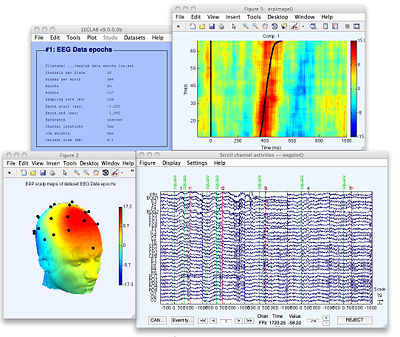
\includegraphics[width=0.5\linewidth]{400px-Eeglab_small.jpg}
            \caption{Diseño metodológico}
            \label{fig:placeholder}
        \end{figure}
        % Fin Código Imagen
        \item Dentro de la carpeta \texttt{MATLAB Drive}, guardar EEGLAB en:  
        \url{User/eeglab\_current/eeglab2024.2/sample\_locs}
        % Código Imágen
        \begin{figure}[h]
            \centering
        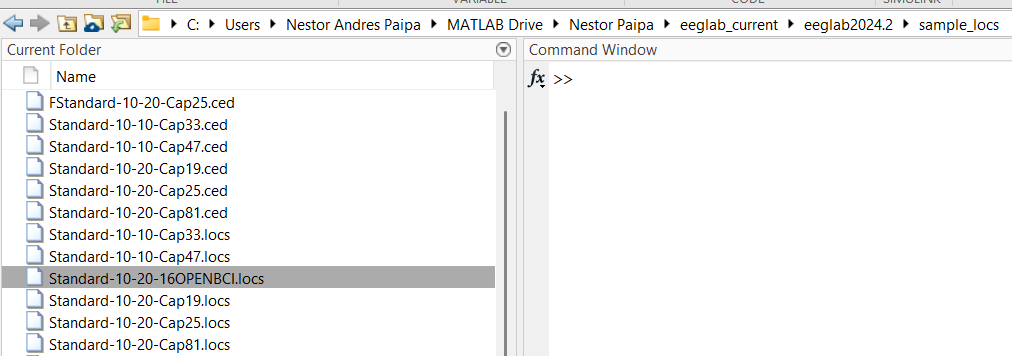
\includegraphics[width=0.6\linewidth]{imagen locs 16.png}
            \caption{Archivo .Locs con las coordenadas del casco de OpenBCI de 16 electrodos}
            \label{fig:placeholder}
        \end{figure}
        % Fin Código Imagen
        
        \item Pegar el archivo con las coordenadas del sistema 10-20 para 16 electrodos:  
        \url{Standard-10-20-16OPENBCI.locs}
        \item Carpeta con recursos:  
        \url{https://github.com/profenapaipa/graficasEEG-AlphaTRP.git}
        \end{itemize}
    \item \textbf{Preparar las sesiones}
        \begin{itemize}
            \item En la carpeta donde está EEGLAB (ejemplo: \texttt{User}), agregar los archivos de las sesiones:  
            \texttt{Sesión 1.txt} y \texttt{Sesión 2.txt}.
            \item Crear un script nuevo llamado: \texttt{comparaciónCanales.m}.
            % Código Imágen
        \begin{figure}[h]
            \centering
        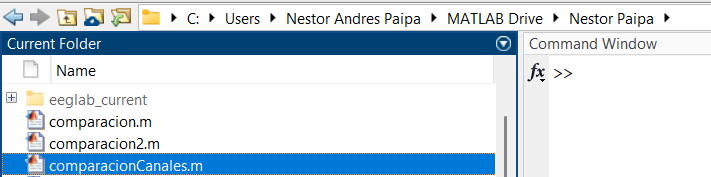
\includegraphics[width=0.6\linewidth]{comparacioncanalesm.png}
            \caption{Creación del Script comparacionCanales.m para generar y agregar el archivo alpha TRP per chanel en el Workspace}
            \label{fig:placeholder}
        \end{figure}
        % Fin Código Imagen
            \item Ejecutar la comparación de canales para generar el archivo:  
            \texttt{alpha\_trp\_per\_channel} en el Workspace.
            \item Al ejecutar se carga automáticamente la variable \texttt{alpha\_trp\_per\_channel}.
             % Código Imágen
        \begin{figure}[h]
            \centering
        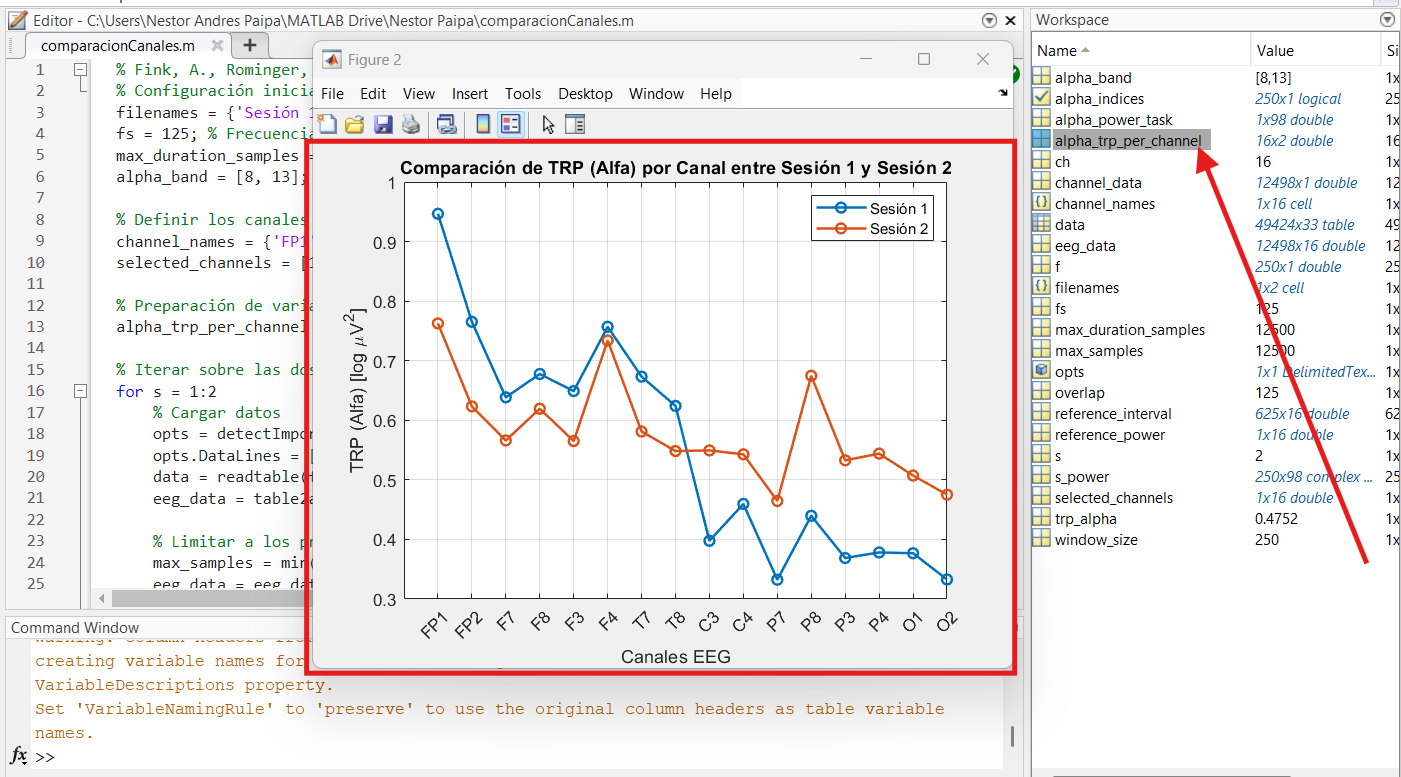
\includegraphics[width=0.6\linewidth]{alphatrpenworkspace.png}
            \caption{Gráfica Alpha TRP en comparación de las Sesiones 1 y 2. A la derecha, la tabla alpha\_trp\_per\_channel agregada al workspace}
            \label{fig:placeholder}
        \end{figure}
        % Fin Código Imagen
        \end{itemize}
        \textbf{Nota: En caso de error al ejecutar EEGLAB. Agregar EEGLAB al path permanentemente:}
        \begin{itemize}
            \item En MATLAB, ir a: \textbf{Home → Set Path}.
            \item Hacer clic en \textbf{Add with Subfolders}.
            \item Seleccionar la carpeta de EEGLAB (ejemplo: \texttt{eeglab2024.2}) en:  
            \texttt{MATLAB Drive/User}.
            \item Guardar y cerrar.
            \item Ahora se podrá ejecutar el comando \texttt{eeglab} desde cualquier carpeta.
        \end{itemize}
    \item \textbf{Ejecutar scripts de mapas topológicos}
        \begin{itemize}
            \item Ejecutar \texttt{egglab2\_16electrodes\_puntos.m}.
             % Código Imágen
        \begin{figure}[h]
            \centering
        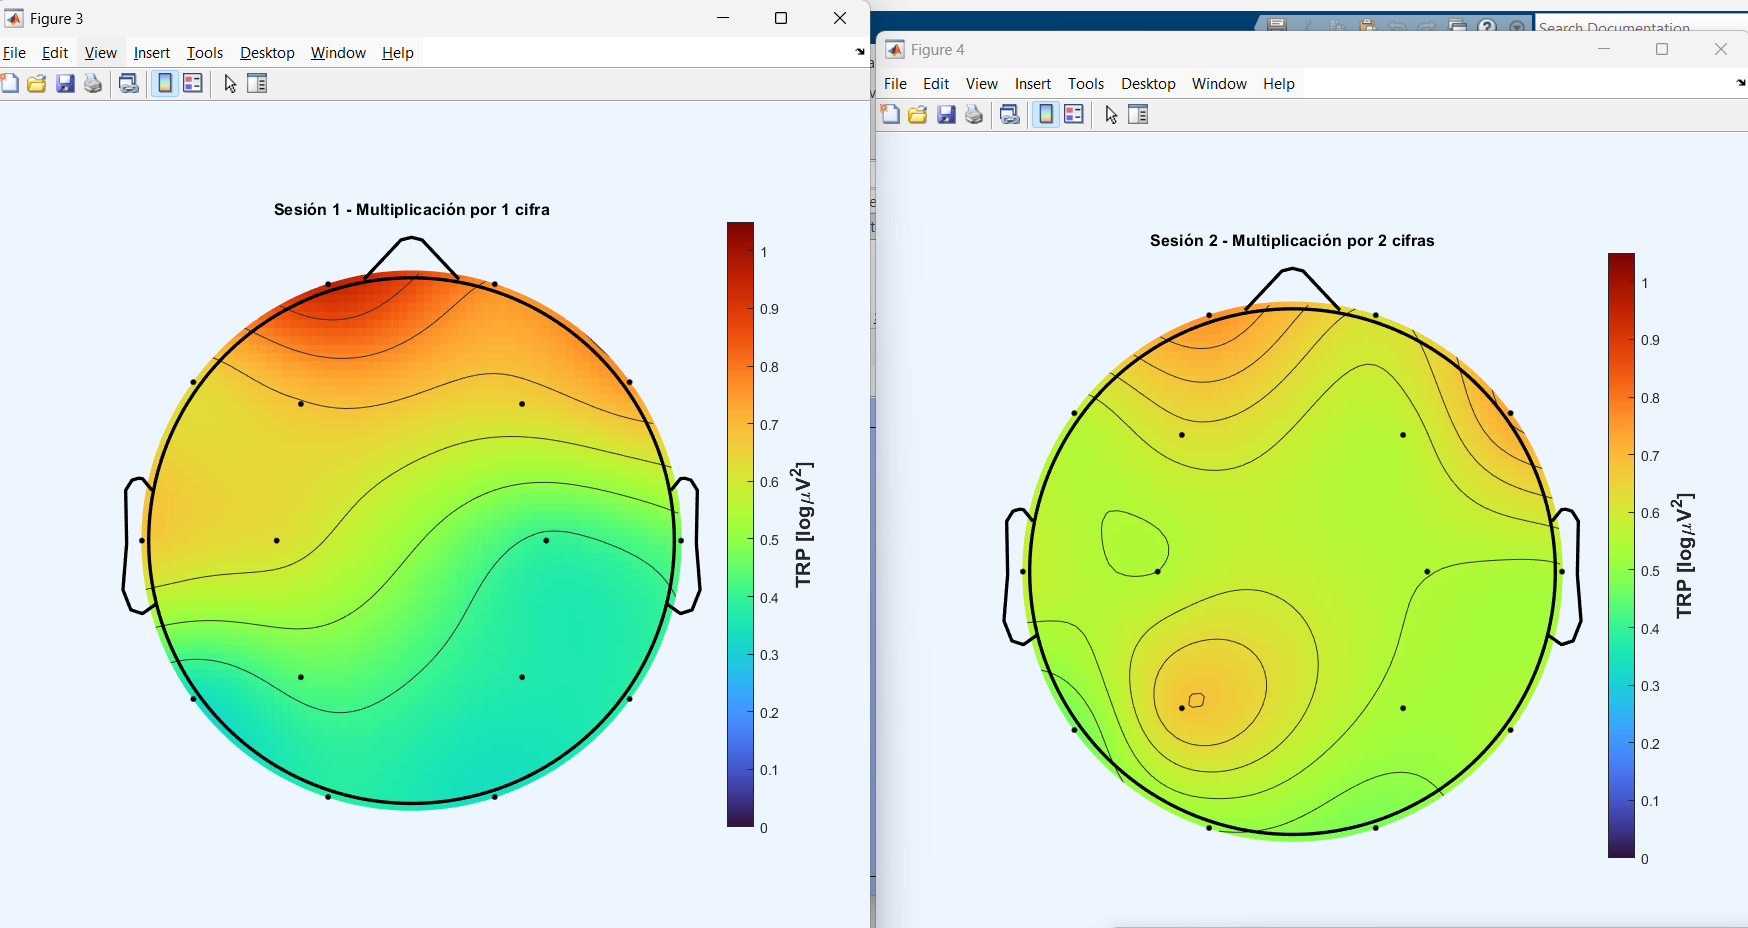
\includegraphics[width=0.6\linewidth]{puntos-mapa.png}
            \caption{Mapa topológico con puntos en las coordenadas de los electrodos}
            \label{fig:placeholder}
        \end{figure}
        % Fin Código Imagen
            \item Ejecutar \texttt{EEGLAB1\_16\_etiquetas.m}.
        \end{itemize}
          % Código Imágen
        \begin{figure}[h]
            \centering
        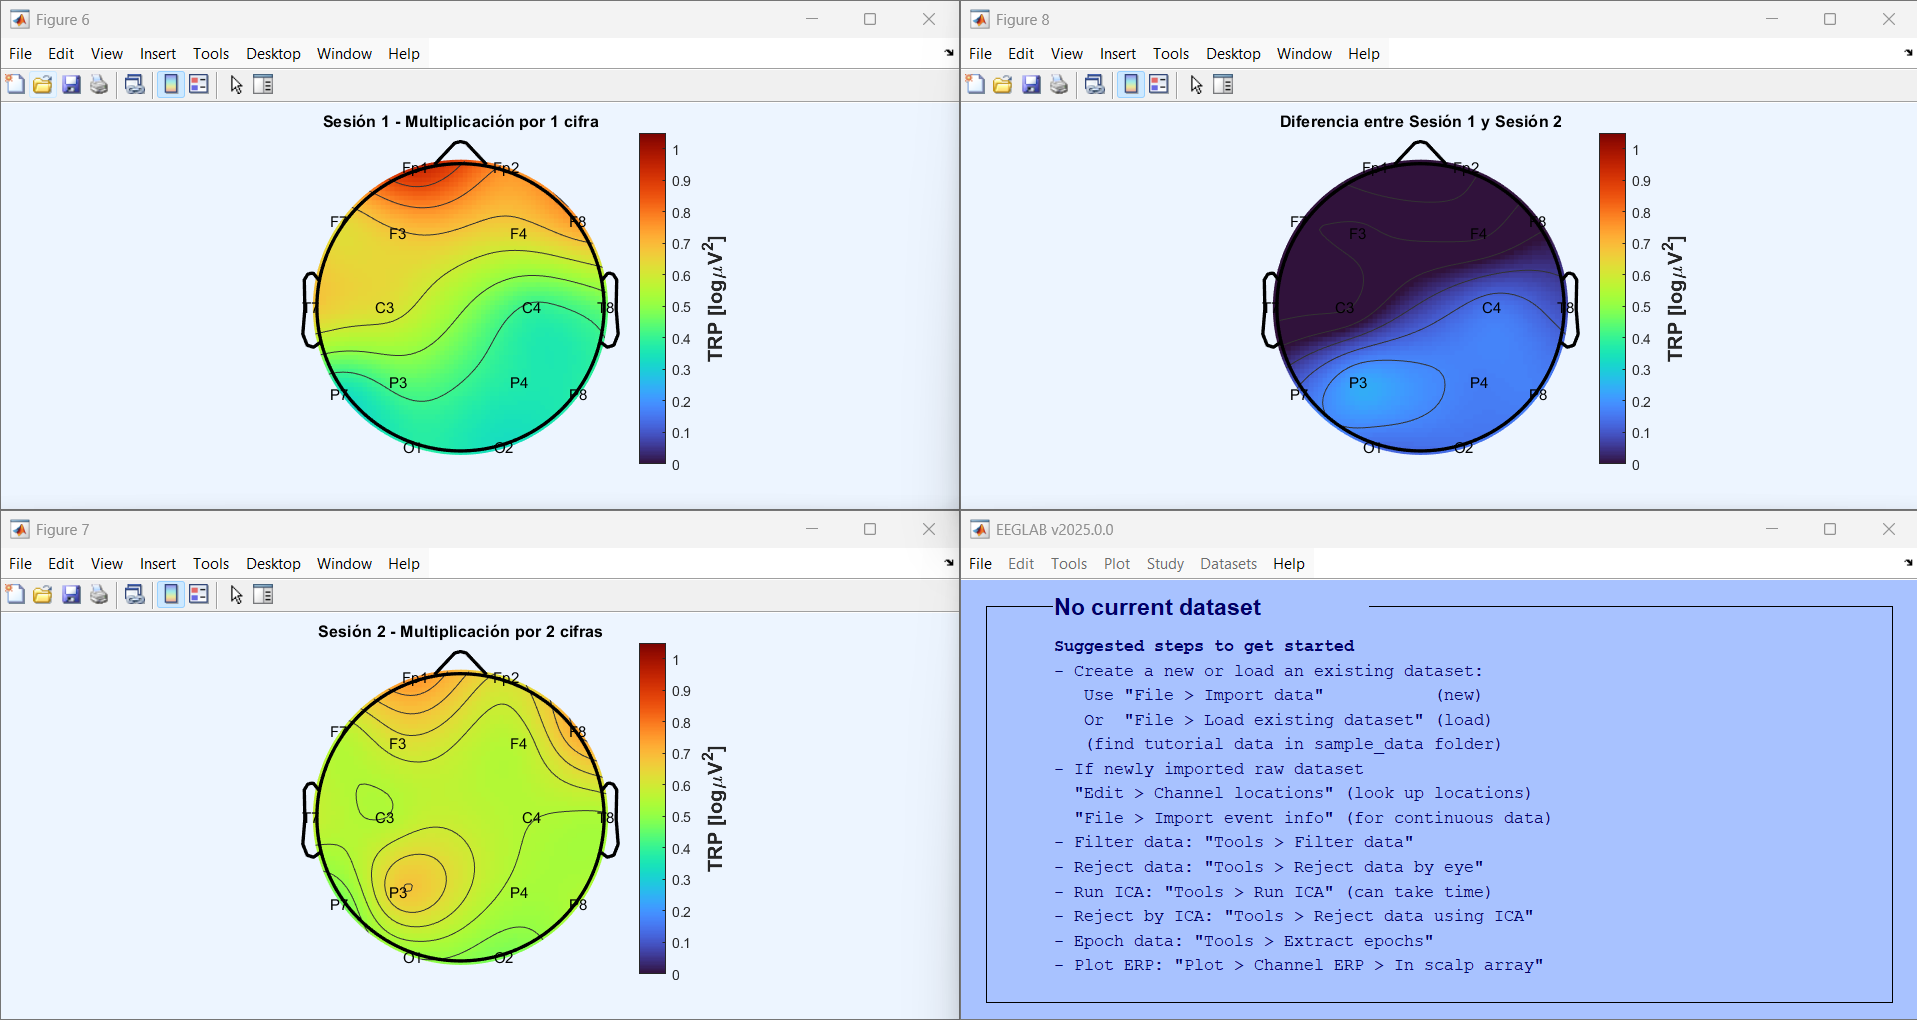
\includegraphics[width=0.6\linewidth]{etiquetas-mapa.png}
            \caption{Mapa topológico con etiquetas con los nombres abreviados en las coordenadas de los electrodos}
            \label{fig:placeholder}
        \end{figure}
        % Fin Código Imagen
    \item \textbf{Comparación entre sesiones}
        \begin{itemize}
            \item Ejecutar \texttt{comparacion.m} para obtener la gráfica de comparación de Alpha TRP entre sesiones.
        \end{itemize}
         % Código Imágen
        \begin{figure}[h]
            \centering
        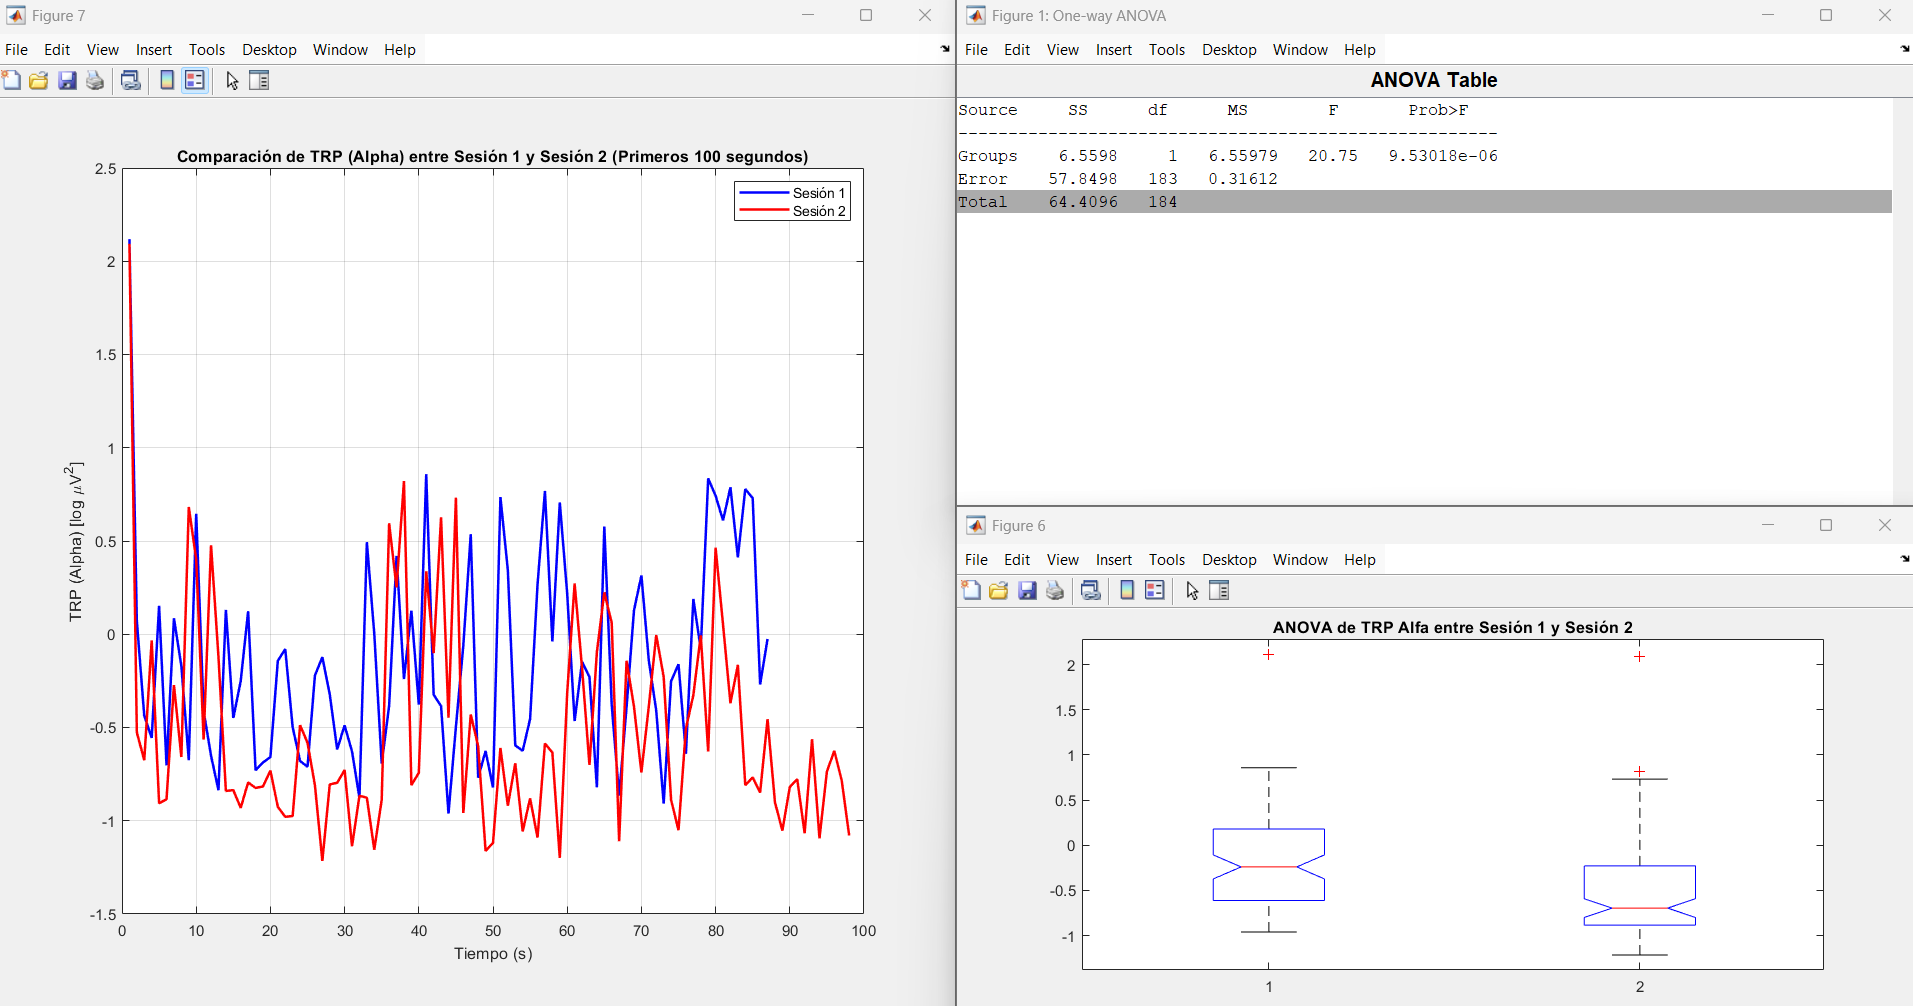
\includegraphics[width=0.6\linewidth]{Comparacionm.png}
            \caption{Gráfica de comparación de Aplha TRP entre las sesiones}
            \label{fig:placeholder}
        \end{figure}
        % Fin Código Imagen
        
    \item \textbf{Comparación entre canales}
        \begin{itemize}
            \item Ejecutar \texttt{comparacion2.m} para obtener la gráfica de Alpha TRP comparado entre canales.
        \end{itemize}
          % Código Imágen
        \begin{figure}[h]
            \centering
        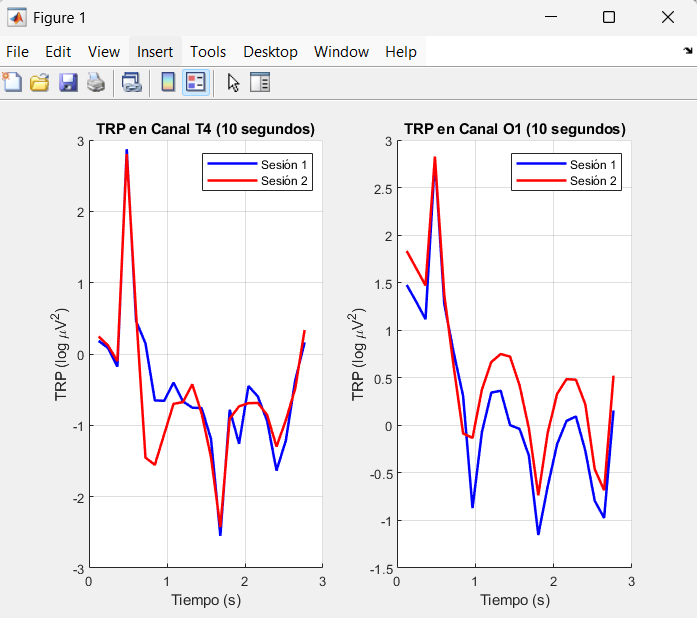
\includegraphics[width=0.6\linewidth]{Comparacion2.png}
            \caption{Gráfica de comparación de Aplha TRP comparado entre electrodos}
            \label{fig:placeholder}
        \end{figure}
        % Fin Código Imagen
\end{enumerate}
\subsection{Guion experimental TEA nivel 1}

Guion experimental definitivo (versión TEA nivel 1).  
\textbf{Objetivo del guion:} Evaluar y favorecer el control inhibitorio (conductual, cognitivo y emocional) en niños con TEA nivel 1 durante la resolución del juego \textit{La Escalera}, empleando interrupciones verbales/gestuales y bloques inteligentes como estímulos controlados.  

\subsubsection*{Fase 1 — Pausar (Interrupciones antes del movimiento)}

\paragraph{Conductual (verbal/gestual)}
\begin{itemize}
    \item Guion verbal breve y literal: ``Espera. Mírala un segundo antes de mover.''  
    \textit{Registro:} si hace pausa (sí/no), latencia para la primera respuesta (ms).
    \item Gesto predecible del investigador: mano colocada cerca del tablero sin tocar.  
    \textit{Registro:} respuesta conductual al gesto (detención, continúa, mirada).
    \item Señal sonora preanunciada y suave (ej.: ding de 200 ms) usada sólo tras explicación previa.  
    \textit{Registro:} cambios en postura, expresión facial.
\end{itemize}

\paragraph{Cognitivo}
\begin{itemize}
    \item Pregunta de recuerdo breve: ``En una frase, ¿cuál es tu plan?''  
    \textit{Registro:} capacidad de síntesis, literalidad.
    \item Pregunta de secuenciación: ``Si mueves ahora, ¿qué harás después?''  
    \textit{Registro:} respuesta correcta/incorrecta, tiempo de respuesta.
    \item Introducción de una ficha neutra similar y consulta: ``¿Cambia esto tu plan?''  
    \textit{Registro:} flexibilidad ante variación mínima.
\end{itemize}

\paragraph{Emocional}
\begin{itemize}
    \item Frase de etiquetado emocional: ``¿Cómo te sientes ahora?'' (opciones visuales disponibles).  
    \textit{Registro:} auto-reporte, signos de angustia.
    \item Pausa estructurada (5--8 s) previamente explicada como parte del procedimiento.  
    \textit{Registro:} tolerancia a la espera.
    \item Oferta explícita de recurso: ``Si quieres, di ‘pausa’ y te damos tiempo.''  
    \textit{Registro:} uso de estrategia de autorregulación.
\end{itemize}

\subsubsection*{Fase 2 — Pensar (Interrupciones durante la planificación)}

\paragraph{Conductual}
\begin{itemize}
    \item Instrucción de presión leve: ``Cuenta hasta tres y dime si sigues con tu plan.''  
    \textit{Registro:} decisión impulsiva vs. reflexiva.
    \item Movimiento lento de una ficha neutra (preacordado con el participante).  
    \textit{Registro:} reconocimiento del cambio, modificación de plan.
    \item Oferta de soporte externo: tarjeta de pasos numerada.  
    \textit{Registro:} uso del soporte y cambio en rendimiento.
\end{itemize}

\paragraph{Cognitivo}
\begin{itemize}
    \item Solicitud de memoria de trabajo verbal: ``Di los dos últimos movimientos.''  
    \textit{Registro:} precisión y latencia.
    \item Presentación de alternativa explícita y petición de valoración crítica.  
    \textit{Registro:} aceptación o rechazo y justificación.
    \item Tarea de visualización: ``Imagínalo 10 s y luego dilo.''  
    \textit{Registro:} calidad de visualización, tiempo.
\end{itemize}

\paragraph{Emocional}
\begin{itemize}
    \item Comentario comparativo neutramente enunciado: ``Otro participante usó X; ¿qué opinas?''  
    \textit{Registro:} reacción emocional, ansiedad social.
    \item Breve regulación guiada: respiración 6 s.  
    \textit{Registro:} cambio en expresión, ritmo respiratorio observable.
    \item Expresión de duda por parte del experimentador: ``No estoy seguro; ¿tú qué piensas?''  
    \textit{Registro:} toma de control o bloqueo.
\end{itemize}

\subsubsection*{Fase 3 — Elegir (Interrupciones justo antes de la ejecución)}

\paragraph{Conductual}
\begin{itemize}
    \item Solicitud de justificación en una frase: ``¿Por qué eliges esto?''  
    \textit{Registro:} capacidad de verbalizar motivos.
    \item Presentación de una opción marcada como ``no recomendada'' y consulta: ``¿Quieres cambiar?''  
    \textit{Registro:} seguimiento de indicaciones y rechazo/aceptación.
    \item Acción experimental controlada: mover y devolver una ficha con explicación clara.  
    \textit{Registro:} reacción a cambios inesperados.
\end{itemize}

\paragraph{Cognitivo}
\begin{itemize}
    \item Pregunta de contingencia: ``Si falla, ¿qué harías luego?''  
    \textit{Registro:} planeamiento alternativo.
    \item Petición de explicación didáctica: ``Si tuvieras que enseñarlo, ¿cómo lo explicarías?''  
    \textit{Registro:} metacognición, estructura del lenguaje.
    \item Oferta temporal: +5 s visibles con cronómetro.  
    \textit{Registro:} uso de tiempo extra.
\end{itemize}

\paragraph{Emocional}
\begin{itemize}
    \item Elogio moderado y neutro: ``Buen intento; respira y decide.''  
    \textit{Registro:} cambio de confianza.
    \item Pregunta anticipatoria: ``¿Te preocupa equivocarte?''  
    \textit{Registro:} anticipación emocional.
    \item Pausa de 3 s con mirada neutra antes de autorizar ejecución.  
    \textit{Registro:} tolerancia al silencio, impulso.
\end{itemize}

\subsubsection*{Indicadores conductuales y registros mínimos}

\begin{itemize}
    \item Tiempo de reacción a interrupción (ms).
    \item Tiempo de decisión (ms).
    \item Número de revisiones/retrocesos.
    \item Errores relativos a la planificación declarada.
    \item Auto-reporte emocional y escalas observacionales (angustia, cooperatividad).
\end{itemize}


\subsubsection{3.4.3. Guión técnico experimental: configuraciones de cubos para Pausar, Pensar y Elegir/Actuar}
\label{subsec:guion_tecnico_experimental}

El guión técnico experimental operacionaliza la regulación del control inhibitorio durante la resolución de problemas matemáticos mediante un sistema de cubos inteligentes que funcionan como agentes multisensoriales autónomos. 

A diferencia de intervenciones basadas en mediación verbal, el presente diseño transfiere la totalidad de la señal reguladora al entorno físico, de manera que las transiciones cognitivas del participante (Pausar, Pensar y Elegir/Actuar) son inducidas exclusivamente mediante tres canales de salida del cubo: luz LED RGB, vibración háptica y señal sonora. 

Las configuraciones se fundamentan en el modelo circumplex (activación × control), permitiendo modular el nivel de activación fisiológica y el grado de guía conductual en cada fase del proceso ejecutivo. Esta estructura técnica traduce el modelo teórico Inhibir–Planificar–Ejecutar en parámetros sensoriales medibles y replicables.

\paragraph{Fase 1: Configuración ``Pausar''}

\textbf{Objetivo funcional:} inducir inhibición motora inicial y estabilización atencional antes de la planificación.

\begin{itemize}
    \item \textbf{Color LED:} Azul claro estático (aprox. RGB 0,150,255).
    \item \textbf{Vibración:} 15\% de intensidad; patrón 200 ms ON / 800 ms OFF.
    \item \textbf{Sonido:} Tono grave suave (100–200 Hz; 300 ms).
    \item \textbf{Duración estándar de fase:} 3–5 s.
\end{itemize}

Esta configuración corresponde al cuadrante de baja activación y alta guía del modelo circumplex. La señal luminosa estable, junto con la vibración rítmica lenta, busca disminuir respuestas impulsivas y favorecer la activación del control inhibitorio motor. Desde el punto de vista neurofisiológico, se espera incremento en actividad theta frontal asociada a regulación ejecutiva temprana y potenciales N2 vinculados a inhibición.

\paragraph{Fase 2: Configuración ``Pensar''}

\textbf{Objetivo funcional:} facilitar la planificación secuencial mediante análisis de medios y fines.

\begin{itemize}
    \item \textbf{Color LED:} Naranja tenue con transición suave (fade in/out de 1 s).
    \item \textbf{Vibración:} 40\% de intensidad; patrón 500 ms ON / 500 ms OFF.
    \item \textbf{Sonido:} Tono medio (400–500 Hz; 200 ms) repetido cada 2 s.
    \item \textbf{Duración estándar de fase:} variable (dependiente del tiempo de planificación del participante).
\end{itemize}

La activación media y el ritmo sensorial constante buscan sostener la memoria de trabajo sin inducir sobreestimulación. Esta configuración se sitúa en un nivel intermedio del circumplex, equilibrando activación y control. Funcionalmente, promueve la inhibición cognitiva de alternativas irrelevantes y la estructuración jerárquica de pasos intermedios. En términos EEG, se prevé aumento de potencia theta frontal y estabilidad en bandas beta durante mantenimiento atencional.

\paragraph{Fase 3: Configuración ``Elegir/Actuar''}

\textbf{Objetivo funcional:} inducir ejecución deliberada y consolidar la decisión tomada.

\begin{itemize}
    \item \textbf{Color LED:} Verde brillante (confirmación) o turquesa (refuerzo positivo).
    \item \textbf{Vibración:} 70–90\% de intensidad; patrón 250 ms ON / 250 ms OFF.
    \item \textbf{Sonido:} Señal ascendente breve o arpegio (500–800 Hz; 400 ms).
    \item \textbf{Duración estándar de fase:} hasta la ejecución motora.
\end{itemize}

Esta fase corresponde al cuadrante de alta activación y alta guía del modelo circumplex. El incremento de intensidad háptica y luminosa busca facilitar la transición de planificación a acción, reforzando la coherencia entre medios previamente estructurados y el fin seleccionado. A nivel neurocognitivo, se anticipa aumento del potencial P3 asociado a toma de decisión y supresión beta previa al movimiento.

\paragraph{Secuencia operativa del ciclo experimental}

Cada problema matemático activa un ciclo completo compuesto por:

\begin{enumerate}
    \item Activación automática del modo ``Pausar''.
    \item Transición programada al modo ``Pensar''.
    \item Activación del modo ``Elegir/Actuar''.
    \item Cierre con luz blanca neutra durante 2 s y vibración desactivada.
\end{enumerate}

La transición entre fases puede ser temporizada o dependiente de eventos conductuales registrados (por ejemplo, detección de movimiento del cubo o interacción física).

\paragraph{Racional técnico-integrador}

La arquitectura sensorial implementada permite traducir constructos ejecutivos abstractos en señales físicas cuantificables. El sistema convierte el entorno en un mediador activo del control inhibitorio, reduciendo la dependencia de instrucción externa y favoreciendo autorregulación progresiva. 

Desde una perspectiva experimental, esta estandarización garantiza replicabilidad, control de variables sensoriales y sincronización precisa con marcadores EEG (N2, theta frontal, P3), permitiendo correlacionar configuraciones del cubo con respuestas neurofisiológicas durante la resolución de problemas matemáticos.



\section{Métricas y Análisis}
\chapter{Resultados}
\chapter{Conclusiones}



\chapter{Trabajos futuros}
\chapter{Bibliografía}
%\printbibliography[title={bibliografia}]
\bibliographystyle{apacite}
\bibliography{bibliografia}

\end{document}
